% Options for packages loaded elsewhere
\PassOptionsToPackage{unicode}{hyperref}
\PassOptionsToPackage{hyphens}{url}
\PassOptionsToPackage{dvipsnames,svgnames,x11names}{xcolor}
%
\documentclass[
  11pt,
  letterpaper,
]{book}

\usepackage{amsmath,amssymb}
\usepackage{iftex}
\ifPDFTeX
  \usepackage[T1]{fontenc}
  \usepackage[utf8]{inputenc}
  \usepackage{textcomp} % provide euro and other symbols
\else % if luatex or xetex
  \usepackage{unicode-math}
  \defaultfontfeatures{Scale=MatchLowercase}
  \defaultfontfeatures[\rmfamily]{Ligatures=TeX,Scale=1}
\fi
\usepackage[]{kpfonts}
\ifPDFTeX\else  
    % xetex/luatex font selection
\fi
% Use upquote if available, for straight quotes in verbatim environments
\IfFileExists{upquote.sty}{\usepackage{upquote}}{}
\IfFileExists{microtype.sty}{% use microtype if available
  \usepackage[]{microtype}
  \UseMicrotypeSet[protrusion]{basicmath} % disable protrusion for tt fonts
}{}
\makeatletter
\@ifundefined{KOMAClassName}{% if non-KOMA class
  \IfFileExists{parskip.sty}{%
    \usepackage{parskip}
  }{% else
    \setlength{\parindent}{0pt}
    \setlength{\parskip}{6pt plus 2pt minus 1pt}}
}{% if KOMA class
  \KOMAoptions{parskip=half}}
\makeatother
\usepackage{xcolor}
\usepackage[lmargin=2.54cm,rmargin=2.54cm,tmargin=2.54cm,bmargin=2.54cm]{geometry}
\setlength{\emergencystretch}{3em} % prevent overfull lines
\setcounter{secnumdepth}{5}
% Make \paragraph and \subparagraph free-standing
\makeatletter
\ifx\paragraph\undefined\else
  \let\oldparagraph\paragraph
  \renewcommand{\paragraph}{
    \@ifstar
      \xxxParagraphStar
      \xxxParagraphNoStar
  }
  \newcommand{\xxxParagraphStar}[1]{\oldparagraph*{#1}\mbox{}}
  \newcommand{\xxxParagraphNoStar}[1]{\oldparagraph{#1}\mbox{}}
\fi
\ifx\subparagraph\undefined\else
  \let\oldsubparagraph\subparagraph
  \renewcommand{\subparagraph}{
    \@ifstar
      \xxxSubParagraphStar
      \xxxSubParagraphNoStar
  }
  \newcommand{\xxxSubParagraphStar}[1]{\oldsubparagraph*{#1}\mbox{}}
  \newcommand{\xxxSubParagraphNoStar}[1]{\oldsubparagraph{#1}\mbox{}}
\fi
\makeatother


\providecommand{\tightlist}{%
  \setlength{\itemsep}{0pt}\setlength{\parskip}{0pt}}\usepackage{longtable,booktabs,array}
\usepackage{calc} % for calculating minipage widths
% Correct order of tables after \paragraph or \subparagraph
\usepackage{etoolbox}
\makeatletter
\patchcmd\longtable{\par}{\if@noskipsec\mbox{}\fi\par}{}{}
\makeatother
% Allow footnotes in longtable head/foot
\IfFileExists{footnotehyper.sty}{\usepackage{footnotehyper}}{\usepackage{footnote}}
\makesavenoteenv{longtable}
\usepackage{graphicx}
\makeatletter
\newsavebox\pandoc@box
\newcommand*\pandocbounded[1]{% scales image to fit in text height/width
  \sbox\pandoc@box{#1}%
  \Gscale@div\@tempa{\textheight}{\dimexpr\ht\pandoc@box+\dp\pandoc@box\relax}%
  \Gscale@div\@tempb{\linewidth}{\wd\pandoc@box}%
  \ifdim\@tempb\p@<\@tempa\p@\let\@tempa\@tempb\fi% select the smaller of both
  \ifdim\@tempa\p@<\p@\scalebox{\@tempa}{\usebox\pandoc@box}%
  \else\usebox{\pandoc@box}%
  \fi%
}
% Set default figure placement to htbp
\def\fps@figure{htbp}
\makeatother
% definitions for citeproc citations
\NewDocumentCommand\citeproctext{}{}
\NewDocumentCommand\citeproc{mm}{%
  \begingroup\def\citeproctext{#2}\cite{#1}\endgroup}
\makeatletter
 % allow citations to break across lines
 \let\@cite@ofmt\@firstofone
 % avoid brackets around text for \cite:
 \def\@biblabel#1{}
 \def\@cite#1#2{{#1\if@tempswa , #2\fi}}
\makeatother
\newlength{\cslhangindent}
\setlength{\cslhangindent}{1.5em}
\newlength{\csllabelwidth}
\setlength{\csllabelwidth}{3em}
\newenvironment{CSLReferences}[2] % #1 hanging-indent, #2 entry-spacing
 {\begin{list}{}{%
  \setlength{\itemindent}{0pt}
  \setlength{\leftmargin}{0pt}
  \setlength{\parsep}{0pt}
  % turn on hanging indent if param 1 is 1
  \ifodd #1
   \setlength{\leftmargin}{\cslhangindent}
   \setlength{\itemindent}{-1\cslhangindent}
  \fi
  % set entry spacing
  \setlength{\itemsep}{#2\baselineskip}}}
 {\end{list}}
\usepackage{calc}
\newcommand{\CSLBlock}[1]{\hfill\break\parbox[t]{\linewidth}{\strut\ignorespaces#1\strut}}
\newcommand{\CSLLeftMargin}[1]{\parbox[t]{\csllabelwidth}{\strut#1\strut}}
\newcommand{\CSLRightInline}[1]{\parbox[t]{\linewidth - \csllabelwidth}{\strut#1\strut}}
\newcommand{\CSLIndent}[1]{\hspace{\cslhangindent}#1}

\usepackage{graphicx}
\usepackage{adjustbox}
\usepackage{fancyhdr}
\pagenumbering{gobble}
\renewcommand{\thefootnote}{\arabic{footnote}}
\setlength{\fboxsep}{3.4mm}
\setlength{\baselineskip}{20pt}
\usepackage{booktabs}
\usepackage{longtable}
\usepackage{array}
\usepackage{multirow}
\usepackage{wrapfig}
\usepackage{float}
\usepackage{colortbl}
\usepackage{pdflscape}
\usepackage{tabu}
\usepackage{threeparttable}
\usepackage{threeparttablex}
\usepackage[normalem]{ulem}
\usepackage{makecell}
\usepackage{xcolor}
\usepackage{booktabs}
\usepackage{graphicx}
\usepackage{adjustbox}
\usepackage{fancyhdr}
\pagenumbering{gobble}
\renewcommand{\thefootnote}{\arabic{footnote}}
\setlength{\fboxsep}{3.4mm}
\setlength{\baselineskip}{20pt}
\makeatletter
\@ifpackageloaded{caption}{}{\usepackage{caption}}
\AtBeginDocument{%
\ifdefined\contentsname
  \renewcommand*\contentsname{Table of contents}
\else
  \newcommand\contentsname{Table of contents}
\fi
\ifdefined\listfigurename
  \renewcommand*\listfigurename{List of Figures}
\else
  \newcommand\listfigurename{List of Figures}
\fi
\ifdefined\listtablename
  \renewcommand*\listtablename{List of Tables}
\else
  \newcommand\listtablename{List of Tables}
\fi
\ifdefined\figurename
  \renewcommand*\figurename{Figure}
\else
  \newcommand\figurename{Figure}
\fi
\ifdefined\tablename
  \renewcommand*\tablename{Table}
\else
  \newcommand\tablename{Table}
\fi
}
\@ifpackageloaded{float}{}{\usepackage{float}}
\floatstyle{ruled}
\@ifundefined{c@chapter}{\newfloat{codelisting}{h}{lop}}{\newfloat{codelisting}{h}{lop}[chapter]}
\floatname{codelisting}{Listing}
\newcommand*\listoflistings{\listof{codelisting}{List of Listings}}
\makeatother
\makeatletter
\makeatother
\makeatletter
\@ifpackageloaded{caption}{}{\usepackage{caption}}
\@ifpackageloaded{subcaption}{}{\usepackage{subcaption}}
\makeatother

\ifLuaTeX
\usepackage[bidi=basic]{babel}
\else
\usepackage[bidi=default]{babel}
\fi
\babelprovide[main,import]{english}
% get rid of language-specific shorthands (see #6817):
\let\LanguageShortHands\languageshorthands
\def\languageshorthands#1{}
\ifLuaTeX
  \usepackage[english]{selnolig} % disable illegal ligatures
\fi
\usepackage{bookmark}

\IfFileExists{xurl.sty}{\usepackage{xurl}}{} % add URL line breaks if available
\urlstyle{same} % disable monospaced font for URLs
\hypersetup{
  pdflang={en},
  colorlinks=true,
  linkcolor={Maroon},
  filecolor={Maroon},
  citecolor={Blue},
  urlcolor={blue},
  pdfcreator={LaTeX via pandoc}}


\author{}
\date{}

\begin{document}
\frontmatter


\mainmatter
\begin{titlepage}
\centering
\vspace*{-4mm}

\includegraphics[width=69.62mm]{/home/joshoacr13/Documentos/TFM/mirna_analysis/miRNA/TFM/Imagenes/logo.png}  % Incluir logo

\vspace{17mm}

\fontsize{28pt}{28pt}\selectfont
\adjustbox{minipage=14.4cm,cfbox=blue,center}{\begin{center} Trabajo Fin de Máster \end{center}}

\vspace{18.7mm}

\fontsize{20pt}{20pt}\selectfont
Función de los microARNs del tejido adiposo subcutáneo en la regulación de la esteatosis hepática.

\baselineskip 20pt
Role of microRNAs from subcutaneous adipose tissue in the regulation of hepatic steatosis.


\vspace*{2cm} 
\baselineskip 36pt
\fontsize{12pt}{12pt}\selectfont
\center{\rm  Autor}

\vspace*{3.65mm} 
\fontsize{18pt}{18pt}\selectfont
\center{José Andrés Castillo Rivas}

\vspace*{1cm}
\baselineskip 36pt
\fontsize{12pt}{12pt}\selectfont
\center{\rm  Directores}

\vspace*{3.56mm}
\fontsize{14pt}{14pt}\selectfont
\center{Silvia Lorente Cebrián - UNIZAR}
\center{José Miguel Arbonés Mainar - IACS}

\vspace*{16.45mm}
\fontsize{12pt}{12pt}\selectfont
\center{Master in Biophysics and Quantitative Biotechnology}

\vspace*{3.56mm}
\fontsize{12pt}{12pt}\selectfont
\center{FACULTAD DE CIENCIAS}\\
2024–2025
\end{titlepage}

\frontmatter

\chapter{Acknowledgments}\label{acknowledgments}

\chapter{Abstract}\label{abstract}

\emph{Background}: Hepatic steatosis arises from excessive triglyceride
sythesis in hepatocytes and correlates with the progression of metabolic
dysfunction-associated steatotic liver disease (MASLD). Molecules
secreted by subcutaneous white adipose tissue (scWAT), such as microRNAs
(miRNAs), appear to influence MASLD by regulating key molecular
pathways. This study aimed to identify miRNA as a potential biomarkers
linked to steatosis in the scWAT of individuals with obesity and varying
degrees of hepatic steatosis.

\emph{Methods}: Subcutaneous white adipose tissue (scWAT) samples were
collected from 78 individuals with obesity undergoing bariatric surgery.
The patients were categorized into four steatosis groups based on liver
fat content: ``\textless5\%'', ``5--33\%'', ``33--66\%'', and
``\textgreater66\%''. Small RNA sequencing data from scWAT were
processed with the \emph{nf-core/smrnaseq pipeline} (v2.4.0), and gene
expression analysis utilized the \emph{DESeq2} and \emph{isomiRs} R
packages.

\emph{Results}: A total of 374 miRNAs were found to be differentially
expressed between patients with obesity with varying degrees of hepatic
steatosis. Among these, two miRNAs (\emph{hsa-miR-372-3p} and
\emph{hsa-miR-144-3p}) remained significant after multiple test
correction. Bioinformatic analysis of predicted target genes revealed
their involvement in pathways related to hepatocellular carcinoma and
hepatitis B. The \emph{in vitro} essays \emph{hsa-miR-372-3p} mimic show
a significance downregulation the mRNA expression of the target gene
\emph{ACACA} and \emph{FAS}, however, \emph{hsa-miR-144-3p} inihibitor
show no significant results on any of the target genes.

\emph{Conclusions}: The differential expression of \emph{hsa-miR-372-3p}
and \emph{hsa-miR-144-3p} in scWAT suggests that these miRNAs may play a
role in the regulation of hepatic steatosis and the progression of
MASLD. Their association with hepatocellular carcinoma and hepatitis B
pathways underscores their potential relevance to liver pathology. These
findings open avenues for research on miRNA profiles as biomarkers or
therapeutic targets for MASLD, with a focus on distinguishing simple
steatosis from advanced disease.

\tableofcontents
\listoftables
\listoffigures

\mainmatter

\chapter{Introduction and
Antecedents}\label{introduction-and-antecedents}

\section{Overview of Hepatic Steatosis and Metabolic dysfunction-
associated steatotic liver
disease}\label{overview-of-hepatic-steatosis-and-metabolic-dysfunction--associated-steatotic-liver-disease}

Hepatic steatosis, defined by the excessive accumulation of
triglycerides within hepatocytes, results from a wide range of factors
that arising from nutritional and metabolic factors, including obesity,
insulin resistence, and dysregulated lipid
metabolism\textsuperscript{{[}1,2{]}}. This excessive accumulation of
lipids triggers a harmful mechanism known as ``lipotoxicity,''
characterized by the toxic effects of lipid intermediates on
hepatocytes, ultimately leading to cell
apoptosis\textsuperscript{{[}3{]}}. Lipotoxicity is a critical driver in
the progression of metabolic dysfunction-associated steatotic liver
disease (MASLD) to metabolic dysfunction-associated steatohepatitis
(MASH)\textsuperscript{{[}4{]}}. Furthermore, hepatic steatosis is a
central feature of steatotic liver disease (SLD), which is categorized
into two main subtypes: alcohol-related liver disease (ALD) and MASLD,
the latter being the predominant form linked to metabolic dysfunction in
the global population\textsuperscript{{[}5{]}}.

MASLD and its more advanced form, metabolic dysfunction-associated
steatohepatitis (MASH), were previously known as nonalcoholic fatty
liver disease (NAFLD) and nonalcoholic steatohepatitis (NASH),
respectively\textsuperscript{{[}4{]}}. MASLD is diagnosed in adults who
exhibit hepatic steatosis, identified through imaging techniques, blood
biomarkers, or liver histology, in conjunction with being overweight or
obese\textsuperscript{{[}6{]}}, or in the presence of type 2 diabetes
mellitus (T2DM) or at least two metabolic risk abnormalities
(hypertension, hyperlipidaemia or insulin
resistance)\textsuperscript{{[}7,8{]}}. Although in many cases it may be
asymptomatic in its early stages, this condition can progress to more
severe stages such as hepatocelular carcinoma (HCC), depending on its
cause\textsuperscript{{[}9{]}}. It encompasses a spectrum of liver
pathologies ranging from simple hepatic steatosis to metabolic
dysfunction-associated steatohepatitis (MASH), which is marked by
lobular inflammation and hepatocellular ballooning, potentially
progressing to fibrosis and cirrhosis, ultimately leading to liver
failure\textsuperscript{{[}10{]}}.

The prevalence of MASLD is affecting more than a third of the adult
population worldwide, making it the most common chronic liver disease
globally\textsuperscript{{[}11{]}}. Among adults, the prevalence (MASLD)
is approximately 30\%\textsuperscript{{[}12{]}}. MASLD is particularly
prevalent in overweight or obese individuals, with a global incidence of
approximately 50\%, rising to nearly 60\% in individuals with type 2
diabetes (T2D)\textsuperscript{{[}13{]}}.

Over the last 30 years, the global prevalence of MASLD has experienced
significant growth, rising from 17.6\% in 1990 to 23.4\% in 2019,
reflecting an average annual increase of approximately 1.0\%. As of
2019, it was estimated that there were around 1.66 billion prevalent
cases of MASLD worldwide\textsuperscript{{[}14{]}}. This condition is
widespread, with the highest rates reported in South America (44\%),
Middle East East and North Africa (36\%) and followed by South Asia
(33\%), South-East Asia (33\%), North America and Australia (31\%), East
Asia (29\%), Asia Pacific regions (28\%) and Western Europe
(25\%)\textsuperscript{{[}12,15{]}}
(Figure~\ref{fig-prevalence_younossi2023global}). Approximately
one-quarter of the European population is affected by this liver
disease\textsuperscript{{[}8{]}}. In Europe, the prevalence of NAFLD
variates between countries ranging from 5\% to
44\%\textsuperscript{{[}16{]}}. Data from Spain reflect similar rates,
indicating a NAFLD prevalence of 25.8\% in the adult
population\textsuperscript{{[}17{]}}.

\begin{figure}[h]

\centering{

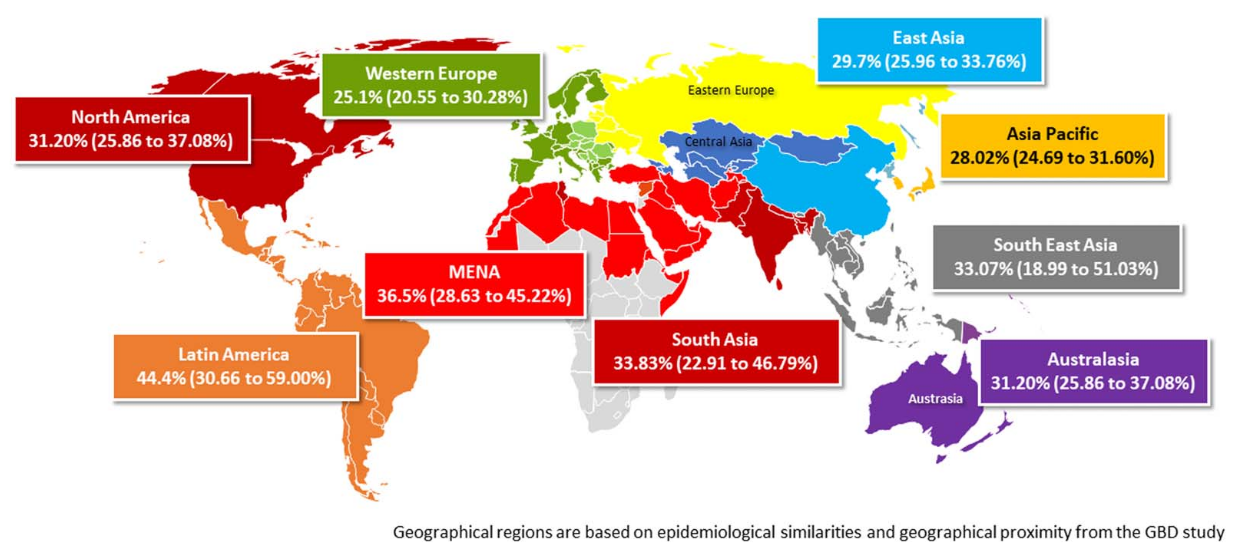
\includegraphics[width=4.11in,height=\textheight,keepaspectratio]{figures/younossi2023global.png}

}

\caption{\label{fig-prevalence_younossi2023global}Prevalence of MASLD
According to Global Regions Data Collected 1990--2019. Image modified
from Younossi \emph{et al.}\textsuperscript{{[}15{]}}}

\end{figure}%

This growing prevalence of MASLD is closely intertwined with the global
rise in obesity and metabolic syndrome, conditions largely influenced by
the complex interplay of adipose tissue function and dysfunction.
Understanding the role of adipose tissue in metabolic regulation is
therefore critical for elucidating the pathophysiology of MASLD.

\section{Role of Adipose Tissue in Metabolic
Regulation}\label{role-of-adipose-tissue-in-metabolic-regulation}

\subsection{Metabolic and Endocrine Functions of Adipose
Tissue}\label{metabolic-and-endocrine-functions-of-adipose-tissue}

Adipose tissue (AT) is a complex and dynamic organ with both metabolic
and endocrine functions\textsuperscript{{[}18{]}}. It plays a pivotal
role in energy balance, insulin sensitivity, immune responses and
overall health\textsuperscript{{[}19{]}}. Its role extends beyond simple
fat storage, influencing whole-body physiology and contributing to
various pathologies, notably obesity and its associated complications
like MASLD\textsuperscript{{[}20{]}}.

\subsection{Types and Location of Adipose
Tissue}\label{types-and-location-of-adipose-tissue}

Adipose tissue in mammals exists in three primary forms: white adipose
tissue (WAT), brown adipose tissue (BAT), and beige or brite
(brown-in-white) adipose tissue. Each type is distinguished by its
unique functions and cellular composition\textsuperscript{{[}21{]}}. WAT
primarily stores energy in the form of lipids, while BAT specializes in
heat production through the uncoupling of oxidative phosphorylation, a
process critical for thermogenesis\textsuperscript{{[}22{]}}. Beige AT,
a metabolically flexible tissue, can transition between energy storage
and thermogenesis depending on physiological needs, highlighting its
role in adaptive responses\textsuperscript{{[}23{]}}
(Figure~\ref{fig-lopez2024unraveling}). The anatomical distribution of
WAT further underscores its functional diversity.

WAT is classified into two major subtypes based its localization and
function:

\begin{itemize}
\item
  Subcutaneous white adipose tissue (scWAT), which constitutes over 80\%
  of total body fat and serves as the primary site for long-term energy
  storage that its located beneath the skin, with its distribution and
  metabolic activity linked to protective effects on overall metabolic
  health\textsuperscript{{[}24{]}}.
\item
  Visceral white adipose tissue (visWAT), which accounts for 10--20\% of
  total body fat in men and 5--10\% in women, is more metabolically
  active, and is strongly associated with adverse health outcomes such
  as insulin resistance and inflammation. visWAT is located surrounding
  internal organs such as the liver and
  intestines\textsuperscript{{[}24--26{]}}.
\end{itemize}

\begin{figure}[H]

\centering{

\pandocbounded{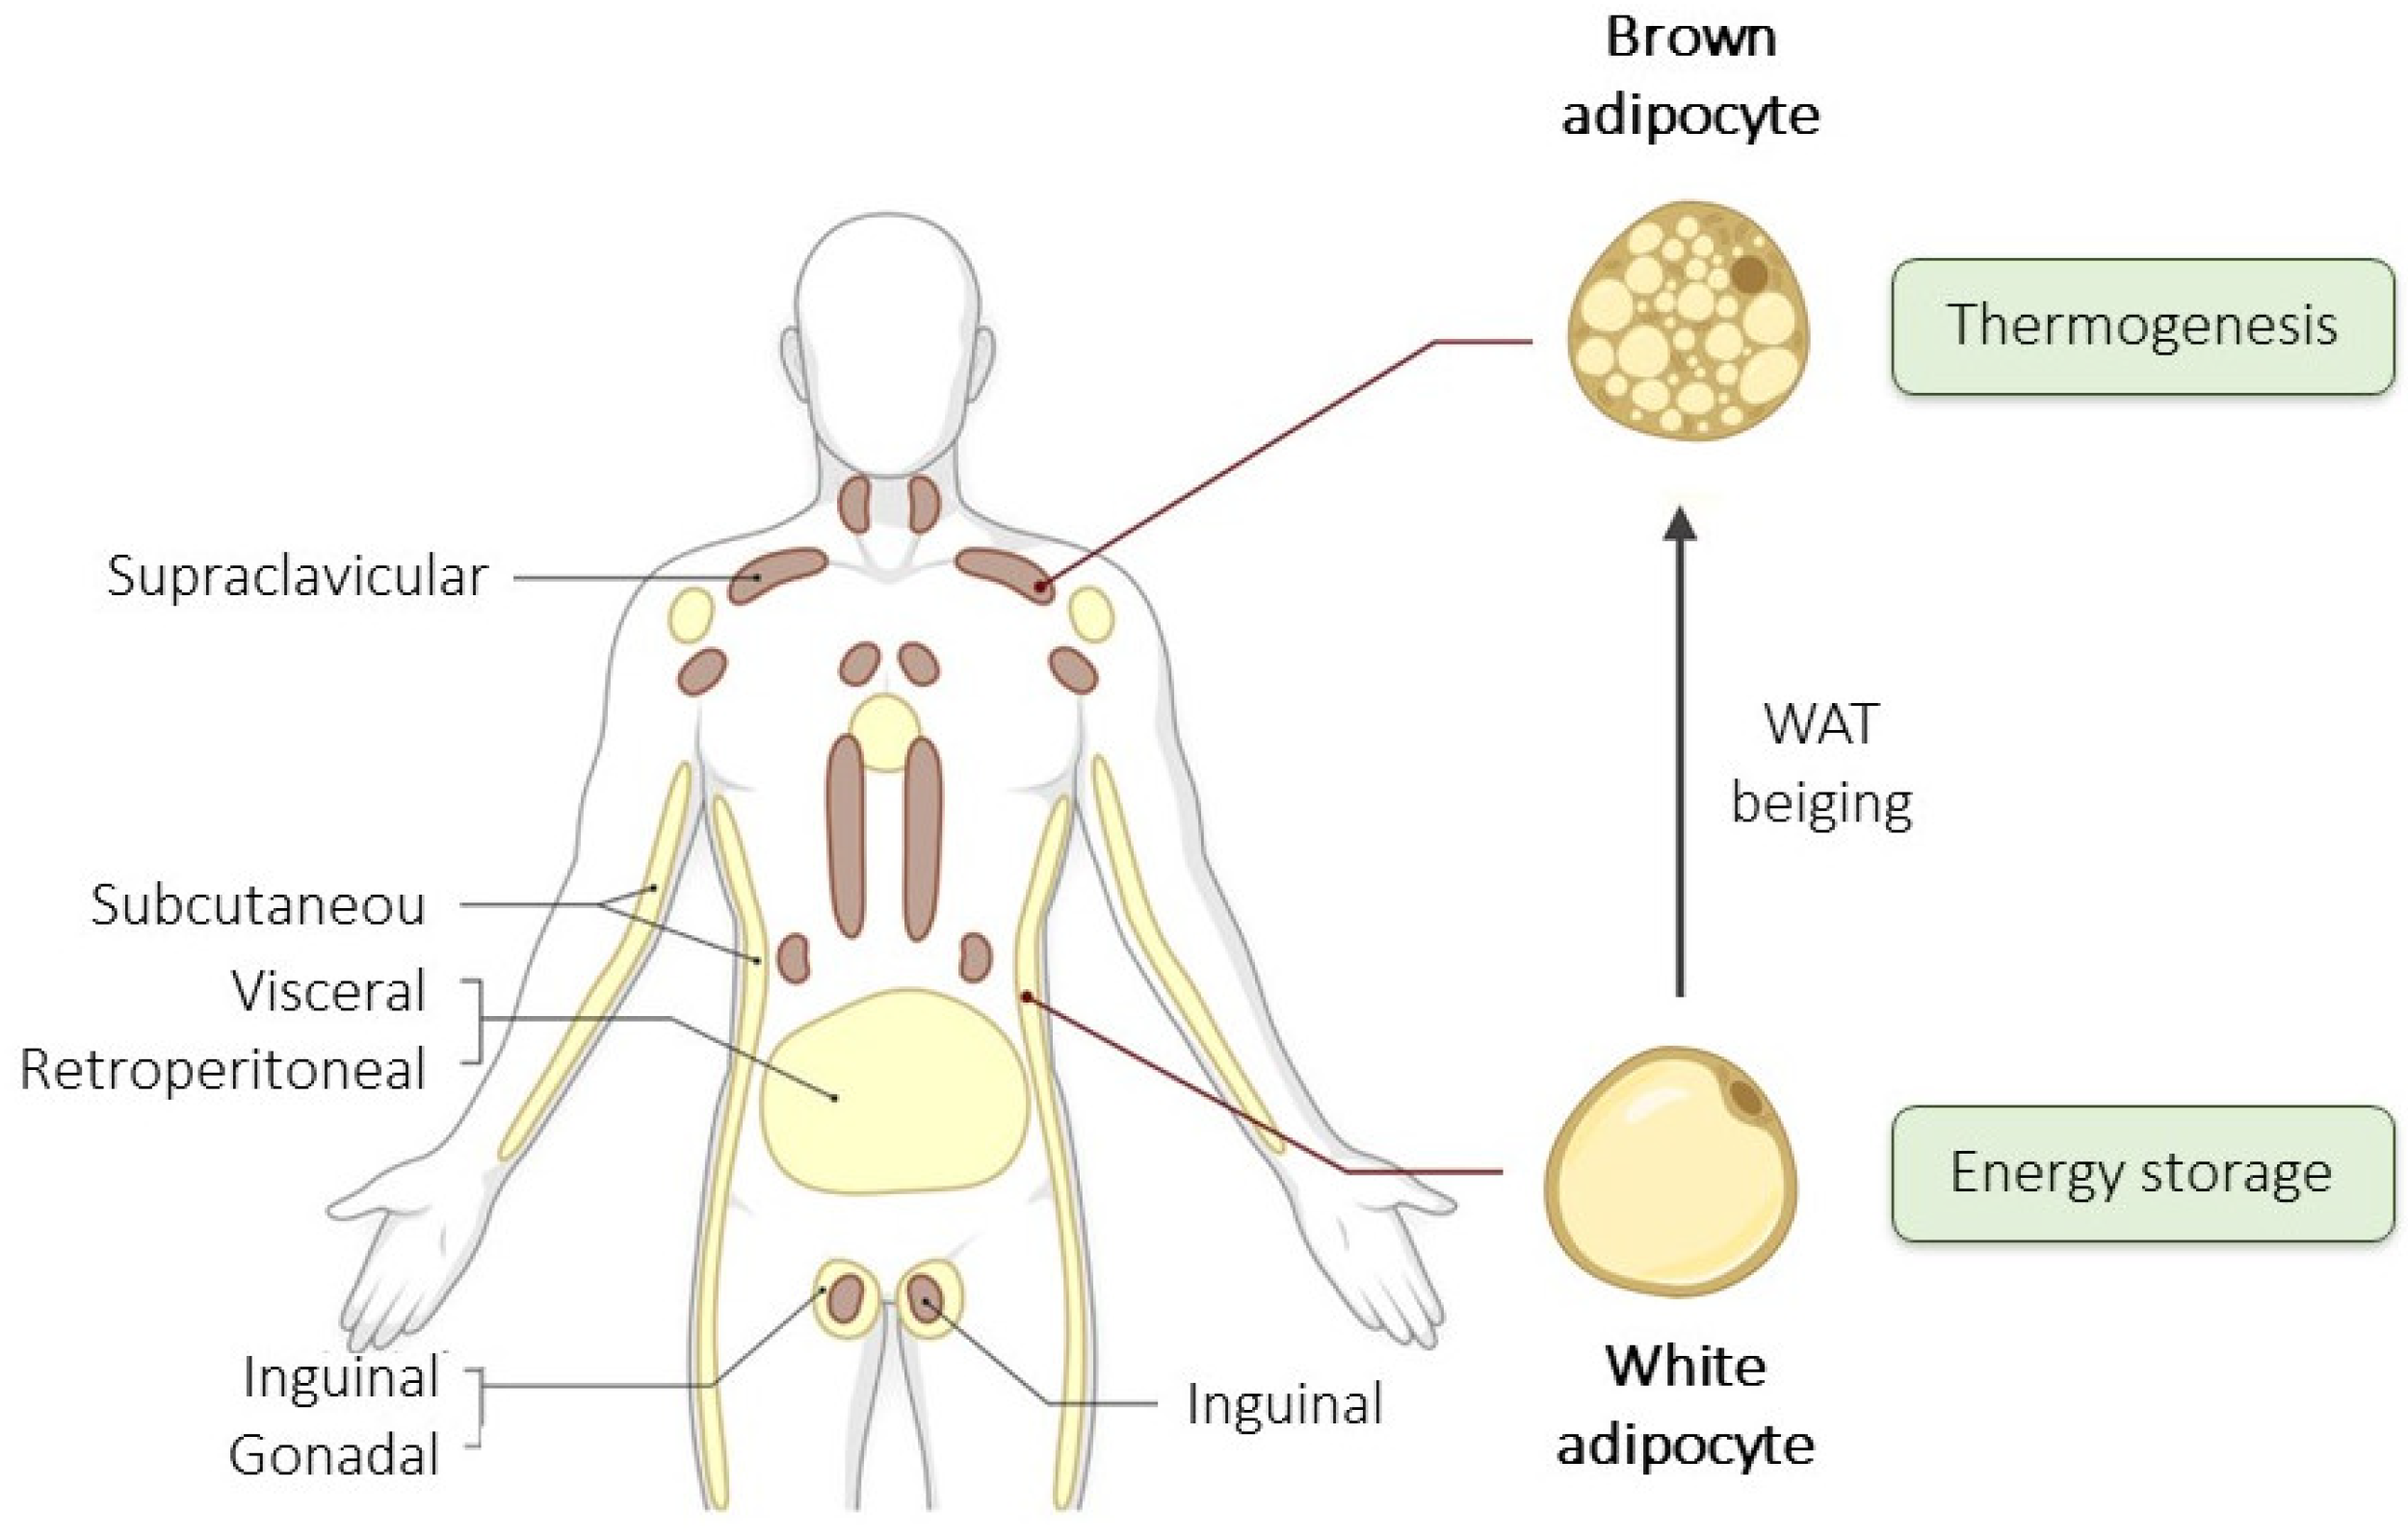
\includegraphics[keepaspectratio]{TFM_files/mediabag/cells-13-00380-g001.png}}

}

\caption{\label{fig-lopez2024unraveling}Adipose tissue distribution in
humans. White adipose tissue (WAT), represented in yellow, is primarily
responsible for energy storage, while brown adipose tissue (BAT), in
brown, is a thermogenic tissue. Image from Lopez-Yus \emph{et
al.}\textsuperscript{{[}23{]}}}

\end{figure}%

\section{Subcutaneous White Adipose Tissue
(scWAT)}\label{subcutaneous-white-adipose-tissue-scwat}

Subcutaneous White Adipose Tissue (scWAT) is including the upper (deep
and shallow abdomen) and lower (gluteofemoral) body
areas\textsuperscript{{[}27{]}}. Under physiological conditions, scWAT
serves as a metabolically inert, long-term triglyceride storage
site\textsuperscript{{[}28{]}}. Acting as a buffer for excess energy,
scWAT protects other organs from ectopic lipid deposition and
contributes to specific metabolic benefits\textsuperscript{{[}21{]}}.
This buffering role allows scWAT to mitigate the impact of excess
dietary lipid consumption while also compensating for energy deficits
during fasting, starvation, or strenuous
exercise\textsuperscript{{[}28{]}}.

scWAT is composed predominantly of adipocytes, which constitute
approximately 50\% of its cellular content\textsuperscript{{[}29{]}}. In
addition to adipocytes, scWAT includes vascular cells, fibroblasts,
adipocyte precursors, multipotent mesenchymal stem-like cells, nerve
cells, and immune cells such as macrophages, lymphocytes, eosinophils,
and mast cells. These components are embedded within an extracellular
matrix that provides structural support\textsuperscript{{[}29{]}}.
Collectively, these cells secrete a wide array of signaling molecules,
including adipokines such as leptin, adiponectin, and resistin, which
play essential roles in maintaining metabolic
homeostasis\textsuperscript{{[}23{]}}.

\section{Metabolic Functions of WAT}\label{metabolic-functions-of-wat}

The main role of white adipose tissue (WAT) is to manage energy balance
by storing and releasing fatty acids (FAs) according to variations in
energy availability\textsuperscript{{[}23{]}}. Furthermore, WAT produces
a range of hormones and cytokines, collectively referred to as
adipokines, which are crucial for regulating numerous physiological
functions\textsuperscript{{[}30{]}}.

\subsection{Lipids Storage and
Mobilization}\label{lipids-storage-and-mobilization}

WAT maintains energy balance by storing and releasing fatty acids (FAs),
a process controlled by the interplay between lipogenesis and lipolysis.
This equilibrium is essential for sustaining energy homeostasis during
periods of fasting or exercise\textsuperscript{{[}23{]}}. In the
Figure~\ref{fig-lopez2024unraveling2} shows these processes in more
detail.

Lipogenesis is the process of synthesizing new lipids from excess
glucose or dietary fatty acids. This process occurs in the cytoplasm of
adipocytes and is tightly regulated by various hormones and
enzymes\textsuperscript{{[}31{]}}. Insulin, the key hormone involved in
this process, facilitates the uptake of glucose and fatty acids into
adipocytes and activates essential enzymes for lipid synthesis,
including acetyl CoA-carboxylase (\emph{ACC}) and fatty acid synthase
(\emph{FAS})\textsuperscript{{[}32{]}}
(Figure~\ref{fig-lopez2024unraveling2}).

Lipolysis, on the other hand, is responsible for breaking down stored
lipids in adipose tissue to release energy for peripheral organs. This
process is particularly important during fasting or exercise when
glucose levels are low, prompting the body to utilize stored fat for
energy\textsuperscript{{[}33{]}}. Lipolysis is regulated by lipases,
which are activated by signals from the sympathetic nervous system,
primarily mediated by norepinephrine, with some influence from
epinephrine. The primary lipases involved include adipose triglyceride
lipase (\emph{ATGL}), hormone-sensitive lipase (\emph{HSL}), and
monoacylglycerol lipase (\emph{MGL})\textsuperscript{{[}34{]}}
(Figure~\ref{fig-lopez2024unraveling2}).

\subsection{Endocrine Function}\label{endocrine-function}

Additionally, WAT secretes various hormones and cytokines, collectively
known as adipokines, which play essential roles in regulating multiple
physiological processes such metabolic, inflammatory, and immune
processes throughout the body\textsuperscript{{[}30{]}}. The endocrine
function of WAT is influenced by nutritional status, physical activity,
hormonal levels, and environmental signals, and is closely related to
its metabolic and storage functions\textsuperscript{{[}35{]}}. The
secretion products are shown in the
Figure~\ref{fig-lopez2024unraveling2}.

Current understanding of adipose tissue (AT)-derived adipokines
encompasses over 100 proteins that interact with various cells and
tissues\textsuperscript{{[}23{]}}. Leptin and adiponectin are the most
characterized and well-studied adipokines. Leptin, the first adipokine
to be discovered, has been shown to influence appetite and energy
expenditure, serving as an important feedback mechanism to the brain
regarding the size and condition of adipose
tissue\textsuperscript{{[}36{]}}. In contrast, adiponectin promotes
insulin sensitivity and fatty acid oxidation in skeletal muscle and the
liver, contributing to the maintenance of glucose and lipid
homeostasis\textsuperscript{{[}37{]}}.

Additionally, WAT releases extracellular vesicles (EVs), small
membrane-bound particles containing various bioactive molecules such as
microRNAs (miRNAs), proteins, and lipids. These EVs play a role in
maintaining energy homeostasis both locally and
systemically\textsuperscript{{[}38,39{]}}.

The endocrine activity of WAT is influenced by factors such as
nutritional status, physical activity, hormonal levels, and
environmental signals. Dysregulation of WAT function, as observed in
obesity and metabolic disorders, can result in insulin resistance (IR),
chronic inflammation, and various metabolic and cardiovascular
complications\textsuperscript{{[}40,41{]}}.

\begin{figure}[H]

\centering{

\pandocbounded{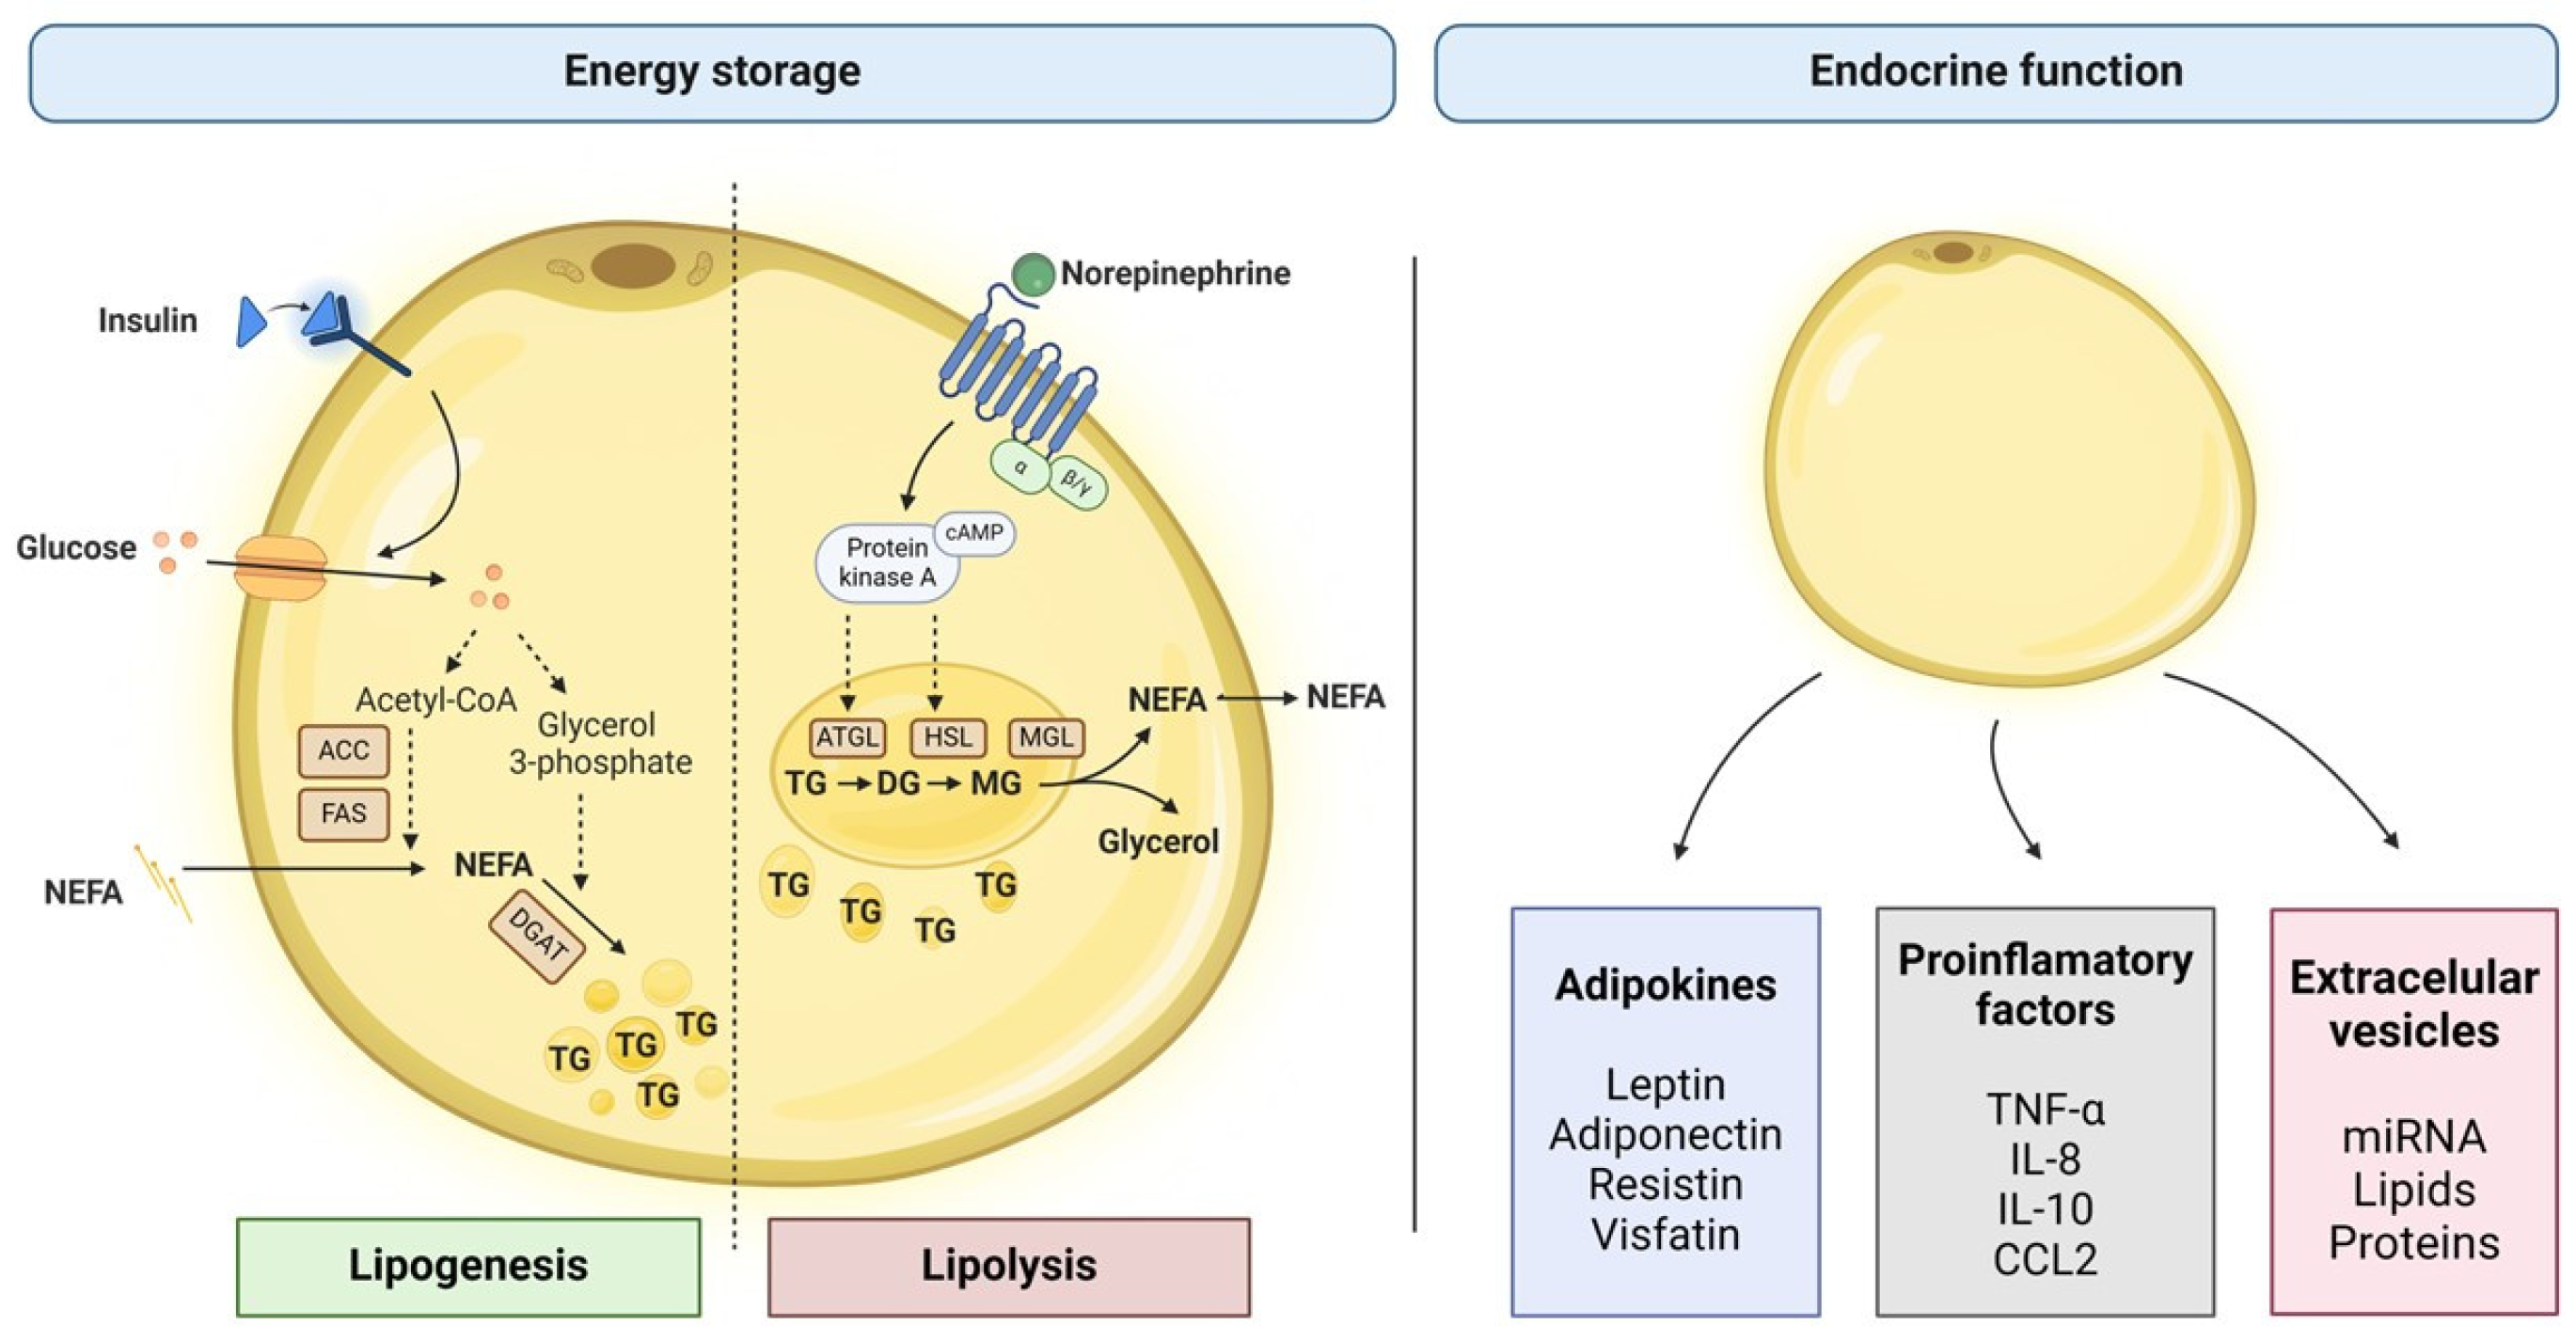
\includegraphics[keepaspectratio]{TFM_files/mediabag/cells-13-00380-g002.png}}

}

\caption[\label{fig-lopez2024unraveling2}Functions of white adipose
tissue (WAT). WAT regulates lipogenesis and lipolysis of non-esterified
fatty acids (NEFA). WAT also secretes a variety of molecules that play
essential roles in the regulation of multiple physiological processes.
Image from Lopez-Yus \textit{et al.}\textsuperscript{{[}23{]}}.
]{\label{fig-lopez2024unraveling2}Functions of white adipose
tissue (WAT). WAT regulates lipogenesis and lipolysis of non-esterified
fatty acids (NEFA). WAT also secretes a variety of molecules that play
essential roles in the regulation of multiple physiological processes.
Image from Lopez-Yus \textit{et al.}\textsuperscript{{[}23{]}}.
\footnotemark{}}

\end{figure}%
\footnotetext{ \textbf{Abbreviations:} \textit{ACC}, acetyl CoA-carboxylase; \textit{ATGL}, adipose triglyceride lipase; \textit{CCL2}, CC-chemokin-ligand-2; \textit{DGAT}, diacylglycerol-O-acyltransferase; \textit{FAS}, fatty acid synthase; \textit{NEFA}, non-esterified fatty acid; \textit{HSL}, hormone-sensitive lipase; \textit{IL-8}, interleukin 8; \textit{IL-10}, interleukin 10; \textit{IMGL}, monoacylglycerol lipase; \textit{TG}, triglyceride; and \textit{TNF-a}, tumor necrosis factor alpha.}

\section{Dysregulation of Adipose Tissue and Its
Implications}\label{dysregulation-of-adipose-tissue-and-its-implications}

Under prolonged positive energy balance, a failure to expand AT mass via
adipocyte hyperplasia (the formation of new adipocytes through precursor
differentiation) results in adipocyte hypertrophy (an increase in cell
size)\textsuperscript{{[}42{]}}. This is a hallmark of AT dysfunction,
as enlarged adipocytes have a diminished capacity to store excess
dietary energy due to being already saturated with
lipids\textsuperscript{{[}43,44{]}}.

As adipocytes grow in size, they experience increased mechanical stress
due to enhanced contact with neighboring cells and components of the
extracellular matrix\textsuperscript{{[}23{]}}. Additionally, adipocytes
face hypoxia, as the hypertrophic expansion of adipose tissue outpaces
angiogenesis\textsuperscript{{[}45{]}}. Furthermore, hypertrophic
adipocytes and damaged cells release pro-inflammatory cytokines, which
recruit and activate immune cells. These factors collectively contribute
to a chronic low-grade inflammatory state in adipose tissue,
significantly impairing its functionality\textsuperscript{{[}46{]}}.

In individuals with obesity, enlarged adipocytes exhibit partial
resistance to the antilipolytic effects of
insulin\textsuperscript{{[}23{]}}. This increased lipolysis results in
elevated levels of free fatty acids (FFAs) in the bloodstream, leading
to ectopic lipid deposition and subsequent lipotoxicity. These
disruptions can contribute to the onset of systemic insulin resistance,
oxidative stress, and the progression of obesity-related
comorbidities\textsuperscript{{[}47{]}}.

The functionality of scWAT is closely linked to body fat
distribution\textsuperscript{{[}23{]}}. Under pathological conditions,
its lipid-storage capacity becomes overwhelmed, leading to hypoxia,
infiltration of pro-inflammatory macrophages, and ectopic fat
accumulation in other tissues, such as the
liver\textsuperscript{{[}48{]}}. These alterations disrupt the balance
of adipokine secretion, fostering a pro-inflammatory state and systemic
insulin resistance, hallmark features in patients with MASLD and related
disorders\textsuperscript{{[}48{]}}.

Understanding the mechanisms underlying scWAT dysfunction highlights the
critical role of adipose tissue expandability in metabolic health. The
ability of adipose tissue to appropriately expand in response to excess
energy intake is crucial for maintaining metabolic homeostasis. When the
expansion capacity is compromised, it contributes to the pathogenesis of
various metabolic diseases, including MASLD.

\section{Adipose Tissue Expandability and Liver Fat
Deposition}\label{adipose-tissue-expandability-and-liver-fat-deposition}

The adipose tissue expandability hypothesis is crucial for understanding
MASLD. This hypothesis posits that the body's capacity to store excess
calories in subcutaneous adipose tissue (scWAT) is limited and varies
between individuals\textsuperscript{{[}49{]}}. Once scWAT reaches its
maximum storage capacity, adipose tissue can no longer effectively store
lipids, leading to the redistribution of lipids to other
organs\textsuperscript{{[}50{]}}. This results in ectopic fat
accumulation, primarily in visceral adipose tissue (visWAT) and the
liver, which contributes to insulin resistance and associated metabolic
complications through mechanisms driven by lipotoxicity and
inflammation\textsuperscript{{[}51{]}}.

The disparity between energy intake and the storage capacity of adipose
tissue is a critical factor in the onset of MASLD. When excessive
caloric intake occurs, particularly in conjunction with the limited
expandability of subcutaneous adipose tissue (scWAT), it results in fat
accumulation in the liver. This hepatic fat buildup, known as steatosis,
is a defining characteristic of MASLD and paves the way for additional
liver damage\textsuperscript{{[}23{]}}.

\subsection{Hepatic Response to Ectopic Fat
Accumulation}\label{hepatic-response-to-ectopic-fat-accumulation}

In MASLD, hepatocytes are the primary cells impacted by ectopic fat
deposition. The buildup of triglycerides in hepatocytes, initially
serving as a protective mechanism against excess circulating free fatty
acids, ultimately results in cellular stress and damage. This fact
manifests in various ways:

\begin{itemize}
\item
  \emph{Inflammatory Response}: The accumulation of ectopic fat in the
  liver triggers an inflammatory response, attracting immune cells and
  producing pro-inflammatory cytokines. Chronic inflammation induces
  notable histological changes, that are critical for the progression of
  the disease from steatosis to MASH and fibrosis, and may also
  contribute to hepatocellular carcinoma
  (HCC)\textsuperscript{{[}52{]}}.
\item
  \emph{Endoplasmic Reticulum (ER) Stress}: The accumulation of lipids
  disrupts ER function in hepatocytes, triggering an unfolded protein
  response that further contributes to cellular stress and
  apoptosis\textsuperscript{{[}53{]}}.
\item
  \emph{Oxidative Stress}: When lipid overflow exceeds the capacities of
  mitochondria and peroxisomes, respiratory oxidation becomes impaired,
  resulting in the generation of harmful metabolites and excess reactive
  oxygen species (ROS)\textsuperscript{{[}54{]}}. These reactive
  molecules cause oxidative stress, worsening necro-inflammatory
  processes in the liver and damaging mitochondria. ROS and oxidized
  low-density lipoproteins (LDL) activate Kupffer and hepatic stellate
  cells, leading to collagen deposition and secondary liver
  fibrosis\textsuperscript{{[}55,56{]}}.
\item
  \emph{Lipotoxicity}: Increased lipid levels, particularly saturated
  fatty acids and harmful lipid species such as diacylglycerol (DAG) and
  ceramide, lead to lipotoxic stress in hepatocytes, causing dysfunction
  and cell death\textsuperscript{{[}57{]}}.
\item
  \emph{Altered Metabolism}: In a fatty liver, hepatocytes exhibit
  changes in carbohydrate and lipid metabolism, often linked to insulin
  resistance. This exacerbates lipid accumulation and impairs liver
  function\textsuperscript{{[}58{]}}.
\end{itemize}

\section{miRNAs and Adipose Tissue
Regulation}\label{mirnas-and-adipose-tissue-regulation}

\subsection{miRNA biology, biogenesis and
function}\label{mirna-biology-biogenesis-and-function}

MicroRNAs (miRNAs) are a highly conserved family of small (21--25
nucleotides) noncoding RNAs\textsuperscript{{[}59,60{]}}. miRNAs are
considered negative regulators of gene expression, functioning by either
suppressing translation or promoting mRNA degradation through base
pairing with complementary sequences in the 3'-untranslated region
(3'-UTR) of protein-coding mRNA transcripts\textsuperscript{{[}61{]}}.
Notably, mRNA degradation constitutes the primary mechanism of miRNA
activity\textsuperscript{{[}62{]}}. miRNAs were first identified in
\emph{Caenorhabditis elegans} by Victor Ambros and Gary Ruvkun, who were
awarded the 2024 Nobel Prize in Physiology or Medicine for their
groundbreaking work on miRNAs\textsuperscript{{[}63--65{]}}.

miRNAs have the ability to regulate hundreds of mRNA targets, and a
single mRNA can be influenced by multiple
miRNAs\textsuperscript{{[}66{]}}. In the human genome, approximately
2,500 miRNAs have been identified\textsuperscript{{[}67{]}}, with about
60\% of protein-coding genes being regulated by miRNAs at the
post-transcriptional level\textsuperscript{{[}68{]}}. Due to this
regulation ability, miRNAs are key regulators within complex genetic
pathways, providing a post-transcriptional layer of control over
homeostatic and developmental processes\textsuperscript{{[}69{]}}. They
play critical roles in a wide range of biological functions, including
the regulation of the cell cycle, proliferation, lipid metabolism,
inflammation, and fibrosis, among others\textsuperscript{{[}70{]}}.
However, the dysregulation of miRNA has been implicated in the
pathogenesis of several many diseases and metabolic disorders, including
MASLD\textsuperscript{{[}71--74{]}}. Specific miRNAs are known to be
differentially expressed in metabolic tissues, including adipose tissue,
in response to pathological states\textsuperscript{{[}69{]}}. Their
potential as biomarkers for disease progression and therapeutic targets
has garnered significant interest in recent
years\textsuperscript{{[}71{]}}.

The biogenesis of miRNAs begins with the maturation of miRNAs occurs
through a multi-step process that begins with transcription by RNA
polymerase II\textsuperscript{{[}75,76{]}}. This enzyme synthesizes
single-stranded, non-protein-coding RNAs, which can be transcribed
either as independent transcripts (intergenic miRNAs), often containing
multiple miRNAs, or derived from the introns of protein-coding genes
(intragenic or intronic miRNAs)\textsuperscript{{[}69{]}}. The
transcription of intergenic miRNAs produces primary miRNAs (pri-miRNAs)
with a distinct hairpin or stem-loop structure and extends 1 kb or much
longer,\textsuperscript{{[}77{]}}, resulting in a long primary
transcript\textsuperscript{{[}78{]}} (Figure~\ref{fig-winter2009many}).

\begin{figure}[H]

\centering{

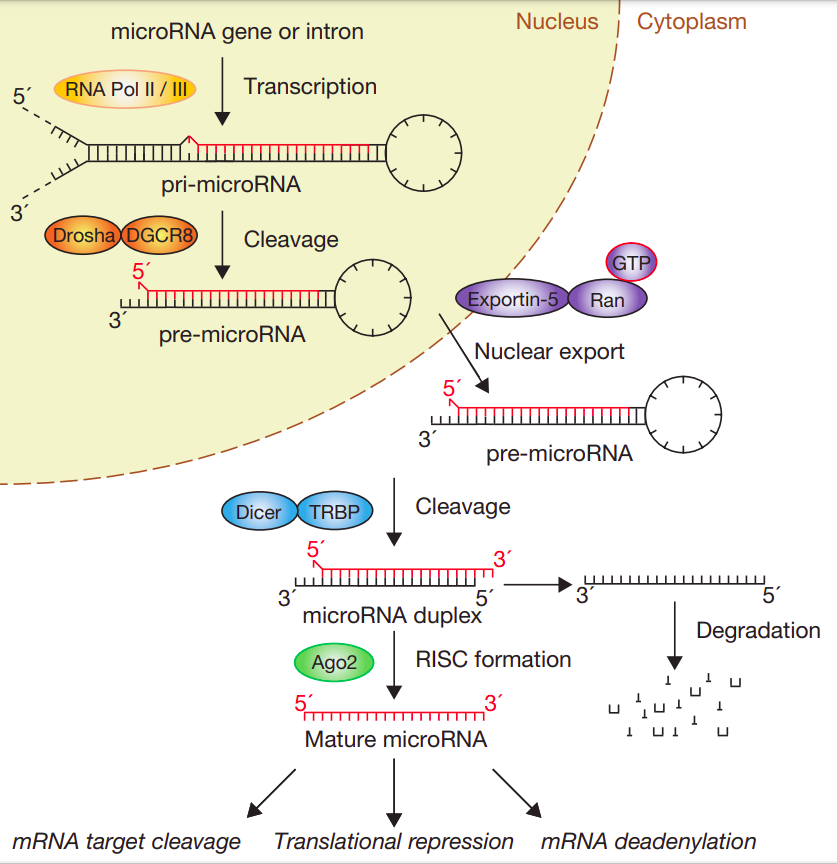
\includegraphics[width=2.79in,height=\textheight,keepaspectratio]{figures/winter2009many.png}

}

\caption{\label{fig-winter2009many}Canonical pathway of miRNA biogenesis
and processing to mature miRNA. Image from Winter \emph{et
al.}\textsuperscript{{[}76{]}}}

\end{figure}%

Then the pri-miRNA is cleaved by ribonulease III-type protein
Drosha\textsuperscript{{[}79{]}} and RNA binding protein DiGeorge
Syndrome Critical Region 8 (DGCR8)\textsuperscript{{[}80{]}} in the
nucleus to produce a \textasciitilde70 nucleotide long hairpin structure
named precursor miRNA (pre-miRNA). Pre-miRNAs are transported to the
cytoplasm by exportin-5, where they are cleaved by the ribonuclease III
enzyme Dicer in complex with TRBP. This cleavage removes the terminal
hairpin structure and generates a \textasciitilde22-nucleotide
miRNA:miRNA* duplex\textsuperscript{{[}81{]}}.

The selection of one strand of the miRNA:miRNA* duplex is influenced by
the thermodynamic stability at the duplex
ends\textsuperscript{{[}75{]}}. This duplex associates with an Argonaute
(AGO) protein to form the RNA-induced silencing complex (RISC). The
mature miRNA is generated when the miRNA* strand is removed from the
duplex. Generally, the strand with lower thermodynamic stability at its
5' end is preferentially loaded into an Argonaute protein (AGO).
Notably, miRNA* is not merely a byproduct of miRNA biogenesis; in many
instances, it functions as a regulatory miRNA\textsuperscript{{[}82{]}}.

The loaded strand, referred to as the guide strand (miRNA), directs the
miRNA-induced silencing complex (miRISC) to the mRNA target. In
contrast, the unloaded strand, known as the passenger strand (miRNA*),
is unwound from the guide strand and subsequently degraded by cellular
machinery\textsuperscript{{[}83,84{]}}.

In addition, the diversity of miRNAs can lead to variations known as
isomiRs, which arise from imprecise cleavage by Drosha and Dicer, 3'
addition events, RNA editing, or single nucleotide polymorphisms
(SNPs)\textsuperscript{{[}84,85{]}}. These isomiRs contribute to the
functional complexity of the miRNA landscape, further expanding the
regulatory potential of miRNAs and highlighting their importance in the
intricate mechanisms of gene regulation.

\subsection{Mechanisms of miRNA-mediated gene
regulation}\label{mechanisms-of-mirna-mediated-gene-regulation}

The interaction between miRNAs and their target mRNAs forms a complex
miRNA-mRNA interactome, where miRNAs bind to various regions of mRNAs.
In the 3' untranslated region (3' UTR), miRNA binding typically induces
transcript degradation or translation inhibition. Interactions in the 5'
UTR and coding regions can also repress gene
expression\textsuperscript{{[}86{]}}. Furthermore, miRNA binding to
promoter regions may induce transcription, although this mechanism
remains poorly understood\textsuperscript{{[}83{]}}.

The classical mechanism of action of the miRNAs involves inhibiting gene
expression by binding to complementary sequences, typically 6--8
nucleotides long, within the 3' untranslated region (3' UTR) of target
mRNAs\textsuperscript{{[}69{]}}. The miRNA strand loaded into Argonaute
(AGO) proteins guides the miRNA-induced silencing complex (miRISC) to
miRNA response elements (MREs) on the target mRNA. The outcome of this
interaction depends on the degree of complementarity: perfect matches
result in transcript degradation, whereas partial complementarity
inhibits gene expression either through mRNA degradation or translation
repression. Interestingly, some miRNAs can act independently of the
miRISC complex. However, the mechanisms underlying these miRISC-free
actions are not yet fully understood and warrant further
investigation\textsuperscript{{[}83,86{]}}.

Due to the requirement for only a 6--8 nucleotide complementarity, a
single miRNA can potentially target hundreds of mRNAs. Typically, one
miRNA targets multiple mRNAs that are interconnected within the same
metabolic pathway. This targeting capability allows miRNAs to regulate
the expression of numerous other miRNAs, thereby contributing to a
complex network of regulatory interactions\textsuperscript{{[}87,88{]}}.
In fact, most mammalian mRNAs are conserved targets of
miRNAs\textsuperscript{{[}89{]}}. Bioinformatic tools have become
essential for predicting and validating miRNA-target interactions,
facilitating the study of miRNA regulatory
networks\textsuperscript{{[}90,91{]}}.

\subsection{Association of miRNA with Hepatic
Steatosis}\label{association-of-mirna-with-hepatic-steatosis}

miRNAs play a critical role in regulating key metabolic pathways in
various liver cell types during the transition from steatosis to
fibrosis, influencing processes such as lipid metabolism, oxidative
stress, inflammation, and fibrosis\textsuperscript{{[}73{]}}. Throughout
the progression of MASLD, miRNAs have been shown to be involved at every
stage of the disease spectrum through diverse regulatory
mechanisms\textsuperscript{{[}72{]}}. This is of considerable intest
providing that they could act as biomarkers of disease prognosis.

Acting as negative posttranscriptional regulators of gene expression,
miRNAs also influence the expression of genes involved in lipid
metabolism.

Given the critical role of miRNAs in regulating metabolic pathways in
the liver, it is essential to explore those specific miRNAs are
associated with hepatic steatosis. These miRNAs can be categorized
according to their primary effects, allowing for a more detailed
understanding of their involvement in this condition

\begin{itemize}
\item
  miRNAs Involved in Lipid Accumulation: \emph{miR-20b} inhibits
  \emph{PPAR}\(\alpha\) reducing free fatty acid oxidation and
  mitochondrial biogenesis, which increases hepatic lipid
  accumulation\textsuperscript{{[}92{]}}. \emph{miR-32} activates sterol
  regulatory element binding protein-mediated adipogenesis, promoting de
  novo lipogenesis and liver lipid
  accumulation\textsuperscript{{[}93{]}}. \emph{miR-30a-3p} upregulates
  lipid metabolism-related proteins and downregulates mitochondrial
  proteins leading to liver fat accumulation\textsuperscript{{[}94{]}} .
  \emph{miR-130b-5p} was found upregulated in MASLD murine models,
  increasing hepatic lipid accumulation via the IGFBP2-dependent AKT
  pathway\textsuperscript{{[}95{]}}. \emph{miR-451a} regulates THRSP,
  reducing triglyceride accumulation in the
  liver\textsuperscript{{[}96{]}}.
\item
  miRNAs Implicated in Insulin Resistance: \emph{miR-188} targets
  \emph{ATG12}, negatively regulating hepatic glucose and lipid
  metabolism, which worsens steatosis and insulin
  resistance\textsuperscript{{[}97{]}}. \emph{miR-27} disrupts
  insulin/AKT signaling by targeting \emph{PDPK1} and \emph{PIK3R1},
  leading to insulin resistance\textsuperscript{{[}98{]}}.
  \emph{miR-30b} induces ER stress by targeting \emph{SERCA2b},
  contributing to insulin resistance\textsuperscript{{[}99{]}}.
  \emph{miR-144} targets Irg1, suppressing the production of itaconate
  and enhancing \emph{SDH} and \emph{FH} activity, which reduces
  fumarate levels, inhibits \emph{NRF2} activation, and impairs the
  antioxidant response, worsening oxidative stress and metabolic
  complications in obesity\textsuperscript{{[}100{]}}.
\item
  miRNAs Regulating Fatty Acid Oxidation: \emph{miR-100} regulates
  directly \emph{CD36}, reducing fatty acid uptake in hepatocytes and
  downstream lipid metabolic
  mediators\textsuperscript{{[}101{]}}.\emph{miR-376b-3p} targets
  \emph{FGFR1}, increasing fatty acid oxidation and improving hepatic
  lipid accumulation\textsuperscript{{[}102{]}}.
\item
  miRNAs Associated with Endoplasmic Reticulum (ER) Stress:
  \emph{miR-26a} mitigates high-fat diet-induced ER stress and steatosis
  by targeting \emph{eIF2}\(\alpha\)\textsuperscript{{[}103{]}}.
\item
  miRNAs Modulating Inflammatory and Fibrotic Pathways: \emph{miR-222}
  regulates mitophagy in hepatic stellate cells (HSCs) by targeting
  \emph{PINK1}, contributing to fibrosis in
  MASH\textsuperscript{{[}104,105{]}}. \emph{miR-146a}: Suppresses
  fibrosis and improves hepatic lipid/glucose metabolism by targeting
  \emph{WNT1} and \emph{WNT5a}\textsuperscript{{[}106,107{]}}.
\item
  miRNAs Affecting Lipogenesis and Lipolysis: \emph{miR-199a-5p} reduces
  \emph{MST1}, modulating hepatic lipogenesis and
  lipolysis\textsuperscript{{[}108{]}}. \emph{miR-103-3p} targets
  \emph{ACOX1}, promoting hepatic steatosis and worsening
  MASLD\textsuperscript{{[}109{]}}. Furthermore, \emph{miR-802} inhibits
  \emph{AMPK} expression, promoting
  NAFL/MASH\textsuperscript{{[}110{]}}.
\item
  Regulatory Insights: Part of the \emph{miR-17-92 cluster}, exacerbates
  steatotic changes by regulating \emph{CYP7A1}
  signaling\textsuperscript{{[}111{]}}. Aditionally, \emph{miR-132} is
  involved in lipid homeostasis by suppressing multiple regulatory
  transcripts\textsuperscript{{[}112{]}}.
\end{itemize}

\begin{longtable}[]{@{}
  >{\centering\arraybackslash}p{(\linewidth - 6\tabcolsep) * \real{0.2000}}
  >{\centering\arraybackslash}p{(\linewidth - 6\tabcolsep) * \real{0.3500}}
  >{\raggedright\arraybackslash}p{(\linewidth - 6\tabcolsep) * \real{0.2000}}
  >{\centering\arraybackslash}p{(\linewidth - 6\tabcolsep) * \real{0.1500}}@{}}
\caption{miRNAs and Their Molecular Targets in Hepatic
Steatosis}\tabularnewline
\toprule\noalign{}
\begin{minipage}[b]{\linewidth}\centering
\textbf{miRNA}
\end{minipage} & \begin{minipage}[b]{\linewidth}\centering
\textbf{Molecular Target}
\end{minipage} & \begin{minipage}[b]{\linewidth}\raggedright
\textbf{Effect}
\end{minipage} & \begin{minipage}[b]{\linewidth}\centering
\textbf{Reference}
\end{minipage} \\
\midrule\noalign{}
\endfirsthead
\toprule\noalign{}
\begin{minipage}[b]{\linewidth}\centering
\textbf{miRNA}
\end{minipage} & \begin{minipage}[b]{\linewidth}\centering
\textbf{Molecular Target}
\end{minipage} & \begin{minipage}[b]{\linewidth}\raggedright
\textbf{Effect}
\end{minipage} & \begin{minipage}[b]{\linewidth}\centering
\textbf{Reference}
\end{minipage} \\
\midrule\noalign{}
\endhead
\bottomrule\noalign{}
\endlastfoot
\emph{miR-20b}

\emph{miR-30a-3p}

\emph{miR-32}

\emph{miR-130b-5p}

\emph{miR-451a} & \emph{PPAR}\(\alpha\) , \emph{ACC},
\emph{p-GSK-3}\(\beta\) , \emph{FASN}, \emph{CPT1}, \emph{p-AMPK},
\emph{UCP2, IGFBP2, INSIG1, THRSP} & Changes in hepatic lipid
accumulation & \textsuperscript{{[}92--96{]}} \\
\emph{miR-27}

\emph{miR-30b}

\emph{miR-144}

\emph{miR-188} & \emph{ATG12, PDPK1}, \emph{PIK3R1, SERCA2b,} Irg1 &
Implicated in insulin resistence & \textsuperscript{{[}97--99{]}} \\
\emph{miR-100}

\emph{miR-376b-3p} & \emph{CD36, FGFR1} & Regulating Fatty Acid
Oxidation & \textsuperscript{{[}101,102{]}} \\
\emph{miR-199a-5p}

\emph{miR-103-3p}

\emph{miR-802} & \emph{MST1,}

\emph{ACOX1}

\emph{AMPK} & Affecting Lipogenesis and Lipolysis: &
\textsuperscript{{[}108--110,113{]}} \\
\emph{miR-222}

\emph{miR-146a} & \emph{ACOX1}, \emph{PINK1, MED1}, \emph{WNT1},
\emph{WNT5a} & Modulating Inflammator and Fibrotic Pathway &
\textsuperscript{{[}104--107{]}} \\
\emph{miR-17} & \emph{CYP7A1} & Steatotic changes &
\textsuperscript{{[}111{]}} \\
\emph{miR-26a} & \emph{eIF2}\(\alpha\) & Endoplasmic Reticulum stress
and high-fat diet-induced steatosis & \textsuperscript{{[}103{]}} \\
\emph{miR-132} & \emph{SIRT1}, \emph{P300}, \emph{PTEN}, \emph{CYP2E1},
\emph{FOXO3} & Lipid homeostasis & \textsuperscript{{[}112{]}} \\
\end{longtable}

\subsection{miRNAs as Biomarkers Based on Omics
Sciences}\label{mirnas-as-biomarkers-based-on-omics-sciences}

The arrival of omics technologies has been essential in advancing
precision medicine by providing an unprecedented ability to analyze
complex biological systems. However, their contribution to the
identification of clinically relevant biomarkers is often indirect,
primarily due to the challenges associated with managing and
interpreting largre datasets\textsuperscript{{[}114{]}}. According to
the World Health Organization, a biomarker is defined as ``any
substance, structure, or process that can be measured in the body or its
products and that can influence or predict the incidence or outcome of a
disease'\,'\textsuperscript{{[}115,116{]}}. Omics technologies, such as
genomics, transcriptomics, and metabolomics, generate massive datasets
that enable the discovery of molecules potentially associated with
disease incidence, prognosis, or therapeutic response. This discovery
process requires subsequent validation using established analytical
techniques such as FISH, RT-PCR, PCR, or immunoaffinity assays before
biomarkers can be approved for clinical use\textsuperscript{{[}114{]}}.
Despite these complexities, the integration of omics data with clinical
insights continues to unlock valuable opportunities for disease
characterization and management.

The ability of a biomarker to provide a detailed characterization of a
disease allows the stratification of patients into well-defined groups
for tailored management and treatment, which forms the foundation of
precision medicine\textsuperscript{{[}117{]}}. Biomarkers can be
categorized into four groups: diagnostic biomarkers, which identify a
specific health condition in a patient; prognostic biomarkers, which
help to chart the progression of a disease; predictive biomarkers, which
suggest the expected response to a specific treatment; and
predisposition biomarkers, which assess the likelihood of developing a
particular illness\textsuperscript{{[}114,117{]}}.

Among emerging biomolecules, miRNAs have gained significant attention as
potential biomarkers\textsuperscript{{[}117{]}}. These small non-coding
RNA molecules are involved in critical cellular processes such as lipid
metabolism, inflammation, and fibrosis, suggesting that they can serve
as monitoring tools for various diseases, including metabolic
dysfunction-associated diseases\textsuperscript{{[}72,118{]}}. miRNAs
are primarily found in the cytoplasm, their presence has also been
confirmed in circulatory system and various bodily fluids, including
saliva and urine\textsuperscript{{[}83{]}}. This occurs due to processes
such as cellular lysis, apoptotic body release, or active secretion.
Their detection in biological fluids highlights their potential as
non-invasive biomarkers for diseases such as MASH and
MASLD\textsuperscript{{[}119{]}}. Their detection in biological fluids
highlights their potential as non-invasive biomarkers for diseases such
as MASH and MASLD\textsuperscript{{[}119{]}}. Circulating miRNAs can be
categorized into three main types: (1) those enclosed within
microvesicles, exosomes, or apoptotic bodies; (2) protein-associated
miRNAs bound to RNA-binding proteins such as AGO2 or HDL; and (3)
free-floating miRNAs
{[}\textsuperscript{{[}83{]}};\textsuperscript{{[}66{]}};
;\textsuperscript{{[}120{]}}{]}. miRNAs have indeed been identified in
adipocytes, which are considered a primary source of exosomal
miRNAs\textsuperscript{{[}118,121{]}}. This diversity underscores their
biological and clinical significance.

A critical advantage of circulating miRNAs is their remarkable stability
in extracellular environments. Their association with proteins or
vesicles protects them from degradation by RNases, allowing for reliable
detection\textsuperscript{{[}122{]}}. Additionally, miRNAs exhibit high
sensitivity and specificity in disease detection, and their measurement
allows multiplex analyses, which further enhances diagnostic precision.
However, challenges remain, such as variability in detection methods,
the need for standardized protocols, and low miRNA abundance in some
cases\textsuperscript{{[}66{]}}. Addressing these barriers through
advancements in absolute quantification methods, exosome-targeting
strategies, and improved extraction techniques will be crucial for
translating miRNA research into clinical
applications\textsuperscript{{[}120{]}}.

Emerging evidence highlights the role of miRNAs in the pathogenesis of
MASLD and its progression to MASH and HCC. Dysregulated miRNA expression
in liver tissue and circulation has been linked to key pathways,
including lipid metabolism, inflammation, fibrosis, and cell
proliferation\textsuperscript{{[}123{]}}. For instance, miR-122 and
miR-34a have been consistently identified as dysregulated in patients
with MASLD, correlating with disease severity and
progression\textsuperscript{{[}119{]}}. These findings suggest that
miRNAs may serve as diagnostic and prognostic biomarkers and even as
therapeutic targets. However, knowledge gaps persist regarding the exact
mechanisms by which miRNAs contribute to disease progression,
particularly in MASH-related hepatocarcinogenesis. Further research is
required to elucidate these pathways and establish causality.

In summary, miRNAs represent a transformative class of biomarkers with
significant potential to reshape precision medicine. Their stability in
extracellular conditions, combined with their presence in readily
accessible fluids, makes them ideal candidates for non-invasive
diagnostics and monitoring. Specific miRNA profiles may enable patient
stratification and personalized treatment strategies, optimizing
therapeutic efficacy while minimizing adverse effects. Advances in omics
technologies, coupled with innovations in bioinformatics and analytical
platforms, are expected to accelerate the integration of miRNAs into
clinical practice.

The present study contributes to this growing field by combining
bioinformatics analyses, in vitro models, and genetic manipulation to
investigate miRNAs associated with hepatic steatosis in patients with
obesity. By identifying miRNAs involved in lipogenesis, lipolysis, and
\(\beta\)-oxidation, this research aims to uncover novel tools for
preventing and treating metabolic disorders such as MASLD and MASH.
Furthermore, the potential to use these miRNAs as non-invasive
biomarkers or therapeutic targets represents a significant advancement
in personalized medicine. This multidimensional approach not only
expands our understanding of metabolic biology but also holds promise
for direct clinical applications, ultimately improving the care of
patients with obesity and associated liver diseases.

\chapter{Hypothesis and Objectives}\label{hypothesis-and-objectives}

\section{Hypothesis}\label{hypothesis}

The main hypothesis of this study is that microRNAs (miRNAs) derived
from subcutaneous adipose tissue might play a key role in regulating
metabolic processes involved in the development and progression of
hepatic steatosis. These miRNAs can alter fundamental metabolic pathways
by modulating genes associated with lipid metabolism in human
hepatocytes.

More specifically, it is proposed that:

\begin{itemize}
\tightlist
\item
  miRNAs secreted or expressed in the subcutaneous adipose tissue of
  patients with obesity, are involved in intercellular communication
  that affects lipid accumulation in the liver, contributing to the
  development of hepatic steatosis.\\
\item
  Bioinformatic analysis of RNAseq data might identify differentially
  expressed miRNAs in the subcutaneous adipose tissue of patients with
  obesity, associated with key metabolic pathways related to
  lipogenesis, lipolysis, and \(\beta\)-oxidation.\\
\item
  The experimental modulation of specific miRNAs in \emph{in vitro}
  cellular models of human hepatocytes, through overexpression or
  inhibition strategies, can reveal their functional role in processes
  related to hepatic steatosis.\\
\item
  The functional characterization of these miRNAs enable their use as
  potential biomarkers or therapeutic targets for the prevention and
  treatment of obesity-associated hepatic steatosis.
\end{itemize}

\section{Main objective}\label{main-objective}

To identify the function of microRNAs (miRNAs) expressed in subcutaneous
adipose tissue in the regulation of metabolic processes involved in the
development of hepatic steatosis, with the aim of these miRNAs could
contitute potential biomarkers and therapeutic targets for obesity
management.

\section{Specific Objectives}\label{specific-objectives}

\begin{enumerate}
\def\labelenumi{\arabic{enumi}.}
\item
  To analyze RNAseq data from subcutaneous adipose tissue of obese
  patients obtained from the FATe cohort (ADIPOFAT).
\item
  To identify a set of differentially expressed miRNAs associated with
  metabolic pathways involved in lipogenesis, \(\beta\)-oxidation, and
  lipolysis related to hepatic steatosis.
\item
  To establish in vitro cell models of human hepatocytes to study the
  function of candidate miRNAs.
\item
  To modify the expression of specific miRNAs through transfection with
  synthetic analogs in an in vitro model of steatosis.
\item
  To evaluate the expression of key genes related to lipogenesis,
  lipolysis, and \(\beta\)-oxidation in miRNA-transfected hepatocytes.
\item
  To explore the potential of identified miRNAs as biomarkers or
  therapeutic targets for the treatment of obesity and its associated
  disorders.
\end{enumerate}

\chapter{Methodological Framework}\label{methodological-framework}

\section{Study Population}\label{study-population}

The analyzed data originates from the FATe
cohort\textsuperscript{{[}124{]}}, a longitudinal study of patients with
obesity undergoing bariatric surgery at Miguel Servet University
Hospital (HUMS, Zaragoza, Spain). For this research, 78 patients with
varying degrees of adiposity were selected based on subcutaneous adipose
tissue (scWAT) samples, which are registered at the regional Biobank
(Biobanco Aragón) and approved by the CEICA ethics committee. Patients
with alcohol or drug abuse, autoimmune diseases, chronic inflammatory
conditions, or infectious diseases (HIV, HBV, HCV) were excluded during
the screening process. The FATe cohort is characterized by a range of
clinical and demographic variables, including sex, age, body mass index
(BMI), steatosis, metabolic dysfunction-associated steatohepatitis
(MASH), hepatocytic ballooning, lobular inflammation, diabetes,
hyperlipidemia, and metabolic dysfunction-associated steatotic liver
disease (MASLD).

\section{Collection and characterization of subcutaneous white adipose
tissue}\label{collection-and-characterization-of-subcutaneous-white-adipose-tissue}

White adipose tissue biopsies (\textasciitilde3 cm³) from the
subcutaneous depot were obtained during laparoscopic bariatric surgery
using a bipolar/ultrasonic device (Thunderbeat). The samples were
extracted through a 12 mm trocar (Applied Medical) inserted into the
left hypochondrium. An experienced pathologist evaluated pathological
features such as steatosis, lobular inflammation, hepatocellular
ballooning, and fibrosis according to the criteria established by the
Nonalcoholic Steatohepatitis Clinical Research Network
(\textsuperscript{{[}125{]}}).

\section{RNA isolation}\label{rna-isolation}

Total RNA was extracted from frozen biopsies of subcutaneous white
adipose tissue (scWAT) and cell cultures using TRIzol (\#T9424, Sigma
Aldrich) following the manufacturer's instructions. For lysing adipose
tissue samples, 1 ml of TRIzol was added \emph{per} sample in a
homogenizer, while for cell cultures, 1 ml of TRIzol was used \emph{per}
10 cm² of the culture plate, along with a scraper. The resulting cell
lysates or tissue disaggregates were transferred to a vial and incubated
for 5 minutes at room temperature to dissociate nuclear components.
Subsequently, 0.2 ml of 100\% chloroform \emph{per} ml of TRIzol was
added. The mixture was shaken vigorously, incubated for 15 minutes at
room temperature, and then centrifuged for 15 minutes at 12,000 g and 4
ºC.

Following centrifugation, three distinct phases were formed. The aqueous
phase, which contained the ribonucleic acids, was collected, and 0.5 ml
of 100\% isopropanol was added to precipitate the RNA. This mixture was
unified, incubated on ice for 10 minutes, and then centrifuged at 12,000
g for 15 minutes at 4 ºC. Afterward, the supernatant was carefully
decanted, and the RNA pellet was resuspended in 1 ml of 75\% ethanol for
washing. The pellet was homogenized and centrifuged at 7,500 g for 5
minutes at 4 ºC. The supernatant was discarded, and the pellet was
allowed to dry for 10 minutes at room temperature. Finally, the RNA was
resuspended in DEPC-treated water. To eliminate any genomic DNA
contamination, all RNA samples were treated with RNase-Free DNase (Life
Technologies). The concentration and purity of the RNA were assessed by
measuring absorbance at 260/280 nm and 260/230 nm using a Nanodrop 2000
(Thermo Fisher Scientific Inc.) and Qubit 4 Fluorometer (Thermo Fisher
Scientific Inc.). The quality of the extracted RNA was visualized using
an agarose gel.

\section{RNA Sequencing}\label{rna-sequencing}

RNA integrity was evaluated using the RNA Integrity Number (RIN) on the
Agilent 2200 TapeStation with the RNA ScreenTape assay. Stranded mRNA
libraries were prepared with the Novogene NGS RNA Library Prep Set
(PT042), which included mRNA isolation using poly-T oligo-attached
magnetic beads, cDNA synthesis, adapter ligation, and PCR amplification.
Libraries that passed quality control checks were sequenced (2x150 bp)
on the Illumina Novaseq X Plus platform.

\section{\texorpdfstring{Analysis of small RNA-seq Data with
\emph{nf-core/smrnaseq}}{Analysis of small RNA-seq Data with nf-core/smrnaseq}}\label{analysis-of-small-rna-seq-data-with-nf-coresmrnaseq}

For the analysis of small RNA sequencing (sRNA-seq) data, version 2.4.0
of the \emph{nf-core/smrnaseq} pipeline\textsuperscript{{[}126{]}} was
used, which is specifically designed for the automated processing of
miRNAs data.

\subsection{\texorpdfstring{Execution of the \emph{nf-core/smrnaseq}
Pipeline}{Execution of the nf-core/smrnaseq Pipeline}}\label{execution-of-the-nf-coresmrnaseq-pipeline}

The installation of \emph{nf-core/smrnaseq} was carried out following
the instructions provided by the authors in
\emph{nf-core}\textsuperscript{{[}127{]}}, available at
\url{https://nf-co.re/smrnaseq/2.4.0} .

To ensure the proper installation and execution of the pipeline, the
following key components were installed beforehand:

\begin{enumerate}
\def\labelenumi{\arabic{enumi}.}
\item
  \emph{Nextflow}: Version 24.04.4 of Nextflow was used, following the
  detailed instructions at \url{https://nf-co.re/usage/installation}.
\item
  \emph{Java Runtime Environment (JRE)}: Version 11.0.25 of the Java
  Runtime Environment was installed, as it is required for compatibility
  with Nextflow and the \emph{nf-core/smrnaseq} pipeline.
\end{enumerate}

To ensure reproducibility and streamline the pipeline execution, one of
the available Docker containers was utilized. These containers provide
the necessary instructions and configurations required to run the
pipeline. The configuration is specified at runtime using the
\texttt{profile} argument. For this analysis, the Docker image
\emph{nf-core/smrnaseq}, available at
\href{https://hub.docker.com/r/nfcore/smrnaseq}{Docker Hub}, was
employed.

The pipeline was executed on a server with 8 CPUs, 16 GB of RAM, and a
Linux operating system. The following command was used in the terminal,
which configures the main options, including the reference genome, input
data, and output file location:

\begin{verbatim}
nextflow run nf-core/smrnaseq -r 2.4.0 
-profile docker,ci  
--genome GRCh38  
--input '/home/joshoacr13/Documentos/TFM/nfcore-smrnaseq/input/samples.csv' 
--fasta 'https://github.com/nf-core/test-datasets/raw/smrnaseq/reference/genome.fa' 
--mirtrace_species 'hsa' 
--outdir /home/joshoacr13/Documentos/TFM/nfcore-smrnaseq/workdir  
-resume -c /home/joshoacr13/Documentos/TFM/nfcore-smrnaseq/nextflow_memory.config 
--filter_contamination 
\end{verbatim}

The pipeline was executed three times to accommodate the large number of
samples, processing 26 samples \emph{per} run.

\subsection{Description of the Parameters
Used}\label{description-of-the-parameters-used}

\begin{itemize}
\item
  \texttt{-profile\ docker,ci}: Runs the pipeline inside a Docker
  container to ensure reproducibility and sets up a continuous
  integration (CI) profile.
\item
  \texttt{-\/-genome\ GRCh38}: Specifies the human genome (version
  GRCh38) as the reference for sequence mapping.
\item
  \texttt{-\/-input}: Provides the path to the CSV file containing
  metadata and the paths to the FASTQ files.
\item
  \texttt{-\/-fasta}: URL to the FASTA file of the reference genome.
\item
  \texttt{-\/-mirtrace\_species\ hsa}: Defines the species as Homo
  sapiens (hsa) for miRNAs analysis with miRTrace.
\item
  \texttt{-\/-outdir}: Sets the working directory for the processed
  results.
\item
  \texttt{-resume}: Allows continuation of a previous analysis without
  restarting from the beginning.
\item
  \texttt{-c}: Specifies a custom configuration file
  (nextflow\_memory.config) to adjust resource usage.
\item
  \texttt{-\/-filter\_contamination}: Enables the contamination
  filtering.
\end{itemize}

\subsection{Analysis Workflow and Tools
Used}\label{analysis-workflow-and-tools-used}

The \emph{nf-core/smrnaseq} pipeline is performed following the next
steps:

\begin{enumerate}
\def\labelenumi{\arabic{enumi}.}
\item
  \textbf{Quality Control} An initial quality assessment of the raw
  reads was conducted using \emph{FastQC} (version
  0.12.1)\textsuperscript{{[}128{]}}. Additionally, 3' adapter trimming
  was performed using \emph{fastp} (version
  0.23.4)\textsuperscript{{[}129{]}}, followed by quality and length
  filtering. A second quality assessment of the trimmed reads was
  conducted with \emph{FastQC}.
\item
  \textbf{miRNA Quality Control}: A more specific quality control
  process for miRNA sequencing was implemented, whereby samples that
  failed to meet the minimum quality thresholds established by
  \emph{miRTrace} (version 1.0.1)\textsuperscript{{[}130{]}} were
  excluded from further analysis. This tool incorporates the following
  steps to ensure the integrity and reliability of the data:
\end{enumerate}

\begin{itemize}
\tightlist
\item
  \textbf{Verify Read Length Distribution}: The majority of reads fell
  within the expected range of 18--24 nucleotides, indicative of
  high-quality small RNA data.
\item
  \textbf{Identify Contaminants}: Potential contaminants such as tRNA,
  rRNA, and other non-target molecules were flagged.
\item
  \textbf{Taxonomic Classification}: Reads were classified taxonomically
  to ensure that most sequences originated from the organism of interest
  (\emph{Homo sapiens}).
\end{itemize}

\begin{enumerate}
\def\labelenumi{\arabic{enumi}.}
\setcounter{enumi}{2}
\tightlist
\item
  \textbf{miRNAs Quantification}:
\end{enumerate}

\begin{itemize}
\tightlist
\item
  \textbf{Alignment}: The filtered reads were aligned against mature
  miRNA sequences in the miRBase database using \emph{Bowtie1} (version
  1.3.1)\textsuperscript{{[}131{]}}. Unmapped reads were aligned against
  ``hairpin'' sequences to identify miRNA precursors.
\item
  \textbf{Post-Alignment Processing}: \emph{SAMtools} (version
  1.16.1)\textsuperscript{{[}132{]}} was used to process the mapping
  results.
\end{itemize}

\begin{enumerate}
\def\labelenumi{\arabic{enumi}.}
\setcounter{enumi}{3}
\item
  \textbf{IsomiR Annotation}: The collapsed reads were processed with
  \emph{mirtop} (version 0.4.28)\textsuperscript{{[}133{]}} to identify
  miRNA variants (isomiRs).
\item
  \textbf{Analysis and Visualization of Results}: The overall pipeline
  metrics, encompassing quality assessments, mapping statistics, and
  expression analysis results, were consolidated and summarized using
  \emph{MultiQC} (version 1.25.1)\textsuperscript{{[}134{]}}.
  Visualization of the results was performed using the \emph{ggplot2}
  package in R\textsuperscript{{[}135{]}}, which facilitated the
  creation of clear and informative graphical representations.
\end{enumerate}

\section{\texorpdfstring{Differential expression analysis according to
steatosis using
\emph{DEseq2}}{Differential expression analysis according to steatosis using DEseq2}}\label{differential-expression-analysis-according-to-steatosis-using-deseq2}

For the differential expression analysis, the R statistical
software\textsuperscript{{[}136{]}}, version 4.4.1 (2024-06-14)
(\url{https://cran.r-project.org/}), was used. This analysis was
performed using the RStudio integrated development environment
(IDE)\textsuperscript{{[}137{]}}, version 2023.12.0+369, designed for
Ubuntu Jammy (\url{https://www.rstudio.com/}).

The script used to perform the differential expression analysis is
available in the file ``\texttt{miRNA\_steatosis.qmd}'' which can be
accessed at the following link:
\url{https://github.com/joshoandres13/miRNAs}.

The analysis began by loading essential R packages: \emph{tidyverse}
(version 2.0.0)\textsuperscript{{[}138{]}} for data manipulation,
\emph{isomiRs}\textsuperscript{{[}139{]}} (version 1.32.1) for analyze
isomirs and miRNAs from sRNA-seq, \emph{DESeq2} (version
1.44.0)\textsuperscript{{[}140{]}} for differential expresion analysis,
\emph{org.Hs.eg.db} (version 3.19.1)\textsuperscript{{[}141{]}} for gene
annotation.

\subsection{Data Preparation}\label{data-preparation}

Metadata were imported, and sample identifiers were stablished as row
names. The variable \emph{Steatosis} is categorized in four distinct
groups. Isomirs count data were subsequently obtained where rows
represent the identified isomiRs and columns correspond to the
experimental samples.

Using isomirs count data and metadata, an object of class
\texttt{IsomirDataSeq} was created. This object enables efficient
management of information derived from small RNA sequencing studies,
streamlining differential expression analyses and facilitating the
interpretation of biological findings.

\subsection{Filtering and Processing of
isomiRs}\label{filtering-and-processing-of-isomirs}

The filtering process enables the grouping of isomiRs into distinct
categories, associating them with a single variant of a miRNA. This
grouping is essential for ensuring consistency and accuracy in
differential expression analyses. To reduce technical noise and
highlight biologically meaningful signals, a stringent filtering
criterion was applied: only isomiRs with a minimum of 20 counts in at
least 40 samples were retained.

\subsection{Differential expression in
scWAT}\label{differential-expression-in-scwat}

In this study, the \emph{DESeq2} package was used to perform
differential expression analysis on scWAT samples with varying degrees
of liver steatosis. The \emph{DESeq2} object was configured using the
Likelihood Ratio Test (LRT), enabling the analysis to account for all
four steatosis categories: \textless5\% (no steatosis), 5--33\% (mild
steatosis), 33--66\% (moderate steatosis), and \textgreater66\% (severe
steatosis). This approach allowed for a comprehensive assessment of gene
expression changes across the entire spectrum of steatosis progression.

\subsubsection{Testing for differential
expression}\label{testing-for-differential-expression}

The criteria for identifying significant differentially expressed miRNAs
across the steatosis categories involved applying a false discovery rate
(FDR) cutoff of less than 0.05. Following the identification of
significant miRNAs, the expression patterns of the selected miRNAs were
further analyzed by representing their normalized counts in boxplots
across the four steatosis groups. This approach enabled the observation
of expression variations of these miRNAs across different steatosis
degrees, offering insights into their potential roles in steatosis
progression. Differences between steatosis groups were evaluated using
the Kruskal-Wallis test

\section{\texorpdfstring{Target mRNA Selection and Validation Using
\emph{multiMiR}}{Target mRNA Selection and Validation Using multiMiR}}\label{target-mrna-selection-and-validation-using-multimir}

The selected miRNAs were used for the identification of mRNA targets
through the \emph{multiMiR} bioinformatics
package\textsuperscript{{[}142,143{]}}, version 2.4.0 in R.
\emph{multiMiR} facilitates a systematic search and annotation of miRNA
targets, providing functional analysis to elucidate biological
mechanisms. For this analysis, only validated interaction data were
utilized.

\subsection{Filtering Parameters}\label{filtering-parameters}

The validated target table provided by \emph{multiMiR} was used during
the selection process. Key columns included:

\begin{enumerate}
\def\labelenumi{\arabic{enumi}.}
\tightlist
\item
  \textbf{database}: Source database of validated interactions, such as
  \emph{miRTarBase}, \emph{TarBase}, or \emph{miRecords}.
\item
  \textbf{mature\_mirna\_id}: Standard format identifier for the miRNA.
\item
  \textbf{target\_symbol}: Target gene symbol.
\item
  \textbf{experiment}: Experimental methods used for validation,
  including luciferase assays, Western blot, or qRT-PCR.
\item
  \textbf{support\_type}: Level of experimental support, such as
  ``Functional MTI'' (miRNA-mRNA functional interaction).
\item
  \textbf{pubmed\_id}: References to PubMed articles reporting the
  interaction.
\item
  \textbf{type}: Specifies whether the interaction is ``validated'' or
  ``predicted.''
\end{enumerate}

\subsection{Selection Criteria}\label{selection-criteria}

To ensure reliable results, databases were filtered according to update
criteria and the following selection parameters:

\begin{itemize}
\item
  Databases up-to-date at the time of analysis were prioritized
  (\emph{miRTarBase} and \emph{TarBase}).
\item
  Only interactions classified as ``validated'' were included.
\item
  Interactions backed by robust experimental methods, such as luciferase
  assays or Western blot, were prioritized.
\item
  Interactions with functional support (``Functional MTI'') and
  verifiable references in PubMed were selected.
\end{itemize}

This approach ensured the identification of mRNA targets with high
reliability and experimental backing, facilitating the analysis of
potential regulatory functions of the studied miRNAs.

\subsection{Functional Analysis}\label{functional-analysis}

To explore the biological functions associated with the validated target
genes, an enrichment analysis was performed using the \emph{KEGGREST}
package\textsuperscript{{[}144{]}} in R. Gene symbols for validated
target genes associated with selected miRNAs were extracted using
\emph{multiMiR} previously, with duplicates removed to ensure a unique
gene list. The Entrez IDs of these genes were mapped to specific
metabolic pathways in KEGG, using parameters that controlled the false
discovery rate (FDR) with the Benjamini-Hochberg method and significance
cutoff values for \texttt{qvalue} and \texttt{pvalue} set at 0.05. The
results included a bar plot displaying the top 5 significantly enriched
KEGG pathways, highlighting their statistical significance and the
number of genes associated with each pathway. This analysis provided
insights into key metabolic pathways and biological processes involving
miRNA-regulated target genes.

\section{Functional validation of
miRNAs}\label{functional-validation-of-mirnas}

\subsection{Cell Culture and Transfections with miRNA
Mimics}\label{cell-culture-and-transfections-with-mirna-mimics}

The human hepatoma HepG2 cell line (American Type Culture Collection,
ATCC® HB-8065™; Manassas, VA, USA) was cultured in an incubator at 37 ºC
and 5\% CO\(_2\) using high-glucose Dulbecco's Modified Eagle Medium
L-GlutaMAX (DMEM) (Gibco, Thermo Fisher Scientific Inc., Waltham, MA,
USA) supplemented with 10\% fetal bovine serum (FBS; Gibco, Thermo
Fisher Scientific Inc., Brazil). Experiments were carried out when the
cells reached 70-80\% confluence.

For the experiments, HepG2 cells were plated at a density of 100,000
cells per well in 12 well-plates for gene expression assays, in DMEM
high-glucose (1 g/L) L-GlutaMAX supplemented with 10\% FBS.

HepG2 cells were reverse-transfected with Lipofectamine RNAiMAX Reagent
(Thermo Fisher Scientific Inc.) and 50 nM of the following mirVana™
synthetic miRNAs (Thermo Fisher Scientific Inc.): a scramble sequence as
a negative control (mirVana™ miRNA Mimic, Negative Control \#1),
negative control (mirVana™ miRNA Inhibitor, Negative Control \#1),
\emph{miR-144-3p} (\(5'-UACAGUAUAGAUGAUGUACU-3'\); assay ID H11051), and
\emph{miR-372-3p} (\(5'-AAAGUGCUGCGACAUUUGAGCGU-3'\); assay ID MC10165).
The miRNA mimics were diluted in Opti-MEM I Reduced Serum Medium (Gibco,
Thermo Fisher Scientific Inc.) and added to the wells according to the
manufacturer's instructions. Following this, Lipofectamine was added to
the wells containing the diluted miRNA mimics and incubated for 15
minutes at room temperature to form miRNA mimic--lipofectamine
complexes. HepG2 cells diluted in DMEM with 10\% FBS were then plated
into the wells. The cells were incubated for 24 hours to assess
transfection efficiency. To induce lipid accumulation and simulate
steatosis\textsuperscript{{[}145{]}}, HepG2 cells were treated with
oleic acid 24 hours after miRNA mimic transfections, mixed in DMEM
GlutaMAX-I supplemented with 10\% FBS, at a final concentration of 0.5
mM used to mimic hepatic steatosis, which reflects the physiological
range of free fatty acids\textsuperscript{{[}146{]}}.

HepG2 cells were frozen on dry ice and stored at -80 °C until RNA
extraction. Cells used for miRNA expression analyses were washed
previously with phosphate-buffered saline (PBS) to completely remove
potential unabsorbed miRNA mimics.

\subsection{Gene Expression Analyses}\label{gene-expression-analyses}

mRNA expression was evaluated in HepG2 cells transfected with miRNA
mimics for 48 h. RNA was reverse transcribed using PrimeScript Reverse
Transcriptase (Takara Bio), with 100 ng of RNA utilized for each
reaction in a total volume of 10 \(\mu\)l. The process was carried out
using an Applied Biosystems 2720 Thermal Cycler, following this
protocol: 10 minutes at 25 °C, 2 hours at 37 °C, and finally, 5 minutes
at 85 °C. The cDNA product were amplified using Quantitative-real time
PCR (qPCR) in a total reaction volume of 15 \(\mu\)l with SYBR Select
Master Mix (Applied Biosystems), to which 0.5 \(\mu\)l of gene-specific
primers at a concentration of 10 \(\mu\)M was added. The primers
utilized are detailed in Table~\ref{tbl-primers} qPCR was performed on a
StepOnePlus system (Applied Biosystems) with the following protocol: an
initial step at 95 °C for 10 minutes, followed by 40 cycles of 15
seconds at 95 °C and 1 minute at 60 °C, concluding with 15 seconds at 95
°C, 1 minute at 60 °C, and a final 15 seconds at 95 °C. The gene
\(\beta\)-actin was used as a housekeeping control to normalize gene
expression levels (\(\triangle Cq\)). Comparisons between gene
expression levels after miRNA mimic transfections
vs.~scramble-sequence-transfected cells (negative control) were
established using the the \(2 -\triangle\triangle CT\) method,
determining relative gene expression\textsuperscript{{[}147{]}}.

\begingroup\fontsize{10.5}{12.5}\selectfont

\begin{longtable}[t]{>{}lll}

\caption{\label{tbl-primers}Primers designed for qPCR mRNA gene
expression analysis}

\tabularnewline

\\
\toprule
\textbf{Gene Name} & \textbf{Forward Primer (5'→ 3')} & \textbf{Reverse Primer (5'→ 3')}\\
\midrule
\em{ACCA} & AGGTGCCTAGAGGGTTGAAGA & TCGGCCCTGCTTTACTAGGT\\
\em{ATGL (PNPLA2)} & TGGAGACTGAGGAGAACAAG & ATCCCTGCTTGCACATCTCT\\
\em{DGAT2} & AGTGGCAATGCTATCATCATCGT & TCTTCTGGACCCATCGGCCCCAGGA\\
\em{FAS} & AAGGACCTGTCTAGGTTTGATGC & TGGCTTCATAGGTGACTTCCA\\
\em{PPARG} & AGATGACAGCGACTTGGCAAT & ACTCAGGGTGGTTCAGCTTC\\
\addlinespace
\em{ACTB-2} & ACCGAGCGCGGCTACAG & CTTAATGTCACGCACGATTTCC\\
\bottomrule

\end{longtable}

\endgroup{}

\vspace{-1em}
\begin{flushleft}
\footnotesize{\textbf{Abbreviations:} 
\textit{ACCA} (Acetyl-CoA Carboxylase Alpha), 
\textit{DGAT2} (Diacylglycerol O-Acyltransferase 2), 
\textit{FAS} (Fatty Acid Synthase), 
\textit{PNPLA2} (Patatin-like phospholipase domain-containing protein 2), 
\textit{PPARG} (Peroxisome Proliferator Activated Receptor Gamma).}
\end{flushleft}

\section{Statistical Analysis}\label{statistical-analysis}

The results are expressed as median {[}interquartile range{]} and number
of cases (\%). Pairwise group comparisons for continuous variables were
calculated using Student's t-test for variables with a Gaussian
distribution and the Mann--Whitney U test for data that do not follow
this distribution. Categorical variables were analyzed using the
chi-square test.

The data obtained from the gene expression experiments were analyzed to
determine the statistical significance of the differences observed
between the experimental groups treated with synthetic miRNAs and the
negative controls. The results are presented as the percentage of
relative regulation (fold change) with respect to the negative control,
expressed as percentages (mean ± standard error of the mean, SEM). The
fold change was calculated by dividing the gene expression of each
sample by the mean expression in the negative control. A Student's
t-test for independent samples was used to evaluate the differences in
the expression of the target genes. Statistical significance was set at
p \textless{} 0.05.

\chapter{Results}\label{results}

\section{Phenotypic Characterization}\label{phenotypic-characterization}

Table~\ref{tbl-description} describes the phenotypical features of FATe
patients selected for this study. This cohort encomprisses 78 subjects
(24\% males; 76\% females), aged between 22 to 61 with obesity as
regards of BMI levels of 46.11 ± 6.13 kg/m². These patients had an
overall presence of general variables/descriptors of metabolic syndrome
features of particular interest those related to liver/hepatic status
(steatosis, lobular inflammation and the prevalence of associated
metabolic diseases). According to the hepatic steatosis scale, 35.9\% of
patients had less than 5\% liver fat, indicating a normal or minimal
steatosis state. A total of 32.1\% exhibited mild steatosis (5--33\%),
while 25.6\% showed moderate fat accumulation (33--66\%). Only 6.4\% of
patients presented severe steatosis (\textgreater66\%), with no
significant differences between men and women (\emph{p}= 0.818).

Regarding lobular inflammation, most patients (66.7\%) had no lobular
inflammation, while 24.4\% exhibited fewer than two foci per microscopic
field, and 3.8\% showed severe inflammation (\textgreater4 foci).
Hepatocyte ballooning analysis revealed that 74.4\% of patients did not
display significant damage, although 9.0\% showed severe ballooning.

Among most prevalent comorbidities, 26.9\% of patients were diagnosed
with diabetes, and 34.6\% presented hyperlipidemia, with the latter
being significantly more prevalent in men (63.2\%) compared to women
(25.4\%, \emph{p}= 0.006). Additionally, 15.4\% of patients were
classified with metabolic dysfunction-associated steatohepatitis (MASH),
although this proportion showed no statistically significant differences
between genders (\emph{p}= 0.249). Collectively, these data highlight
the heterogeneity in the clinical characteristics of the cohort,
emphasizing the complexity of the metabolic relationship between obesity
and liver disease in this cohort.

\section{Quality Control (QC) and reads
preprocessing}\label{quality-control-qc-and-reads-preprocessing}

All QC results from the various steps in the \emph{nf-core/smrnaseq}
pipeline are summarized in the following figures and tables. The
evaluation of samples, both before and after processing, was conducted
using \emph{fastp}, a rapid tool designed for preprocessing RNA
sequencing data. This tool includes features for adapter trimming,
quality filtering, and report generation, making it essential for
assessing sample quality. Overall, Table~\ref{tbl-metrics} presents a
descriptive analysis that includes key metrics related to the sequencing
data.

\clearpage

\begingroup\fontsize{10.5}{12.5}\selectfont

\begin{longtable}{lllll}

\caption{\label{tbl-description}Clinical characteristics of the FATe
cohort}

\tabularnewline

\toprule
\textbf{Characteristic} & \textbf{Overall (n=78)} & \textbf{Female (n=59)} & \textbf{Male (n=19)} & \textbf{p}\\
\midrule
Age (years) median & 47.03 [13.75] & 46.53 [13] & 48.58 [14] & 0.408\\
Body Mass Index (kg/m²) median & 46.11 [8.70] & 45.68 [8.76] & 47.42 [8.70] & 0.284\\
MASLD Activity Score Category (\%): &  &  &  & 0.510\\
- 0 & 22 (28.2) & 16 (27.1) & 6 (31.6) & \\
- 1 & 16 (20.5) & 13 (22.0) & 3 (15.8) & \\
\addlinespace
- 2 & 17 (21.8) & 14 (23.7) & 3 (15.8) & \\
- 3 & 9 (11.5) & 7 (11.9) & 2 (10.5) & \\
- 4 & 9 (11.5) & 7 (11.9) & 2 (10.5) & \\
- >= 5 & 5 (6.4) & 2 (3.4) & 3 (15.8) & \\
Hepatic Steatosis Scale (\%): &  &  &  & 0.818\\
\addlinespace
- < 5\% & 28 (35.9) & 21 (35.6) & 7 (36.8) & \\
- 5-33\% & 25 (32.1) & 20 (33.9) & 5 (26.3) & \\
- > 33-66\% & 20 (25.6) & 15 (25.4) & 5 (26.3) & \\
- > 66\% & 5 (6.4) & 3 (5.1) & 2 (10.5) & \\
Hepatocytic ballooning Category (\%): &  &  &  & 0.489\\
\addlinespace
- None & 58 (74.4) & 45 (76.3) & 13 (68.4) & \\
- Few cells & 13 (16.7) & 10 (16.9) & 3 (15.8) & \\
- Many cells & 7 (9.0) & 4 (6.8) & 3 (15.8) & \\
Lobular Inflammation Category (\%): &  &  &  & 0.596\\
- No foci & 52 (66.7) & 41 (69.5) & 11 (57.9) & \\
\addlinespace
- < 2 foci/200x & 19 (24.4) & 14 (23.7) & 5 (26.3) & \\
- 2-4 foci/200x & 4 (5.1) & 2 (3.4) & 2 (10.5) & \\
- > 4 foci/200x & 3 (3.8) & 2 (3.4) & 1 (5.3) & \\
Diabetes: &  &  &  & 1.000\\
- Yes (\%) & 21 (26.9) & 16 (27.1) & 5 (26.3) & \\
\addlinespace
- No (\%) & 57 (73.1) & 43 (72.9) & 14 (73.7) & \\
Hyperlipidemia: &  &  &  & 0.006\\
- Yes (\%) & 27 (34.6) & 15 (25.4) & 12 (63.2) & \\
- No (\%) & 51 (65.4) & 44 (74.6) & 7 (36.8) & \\
Metabolic dysfunction-associated: &  &  &  & 0.249\\
\addlinespace
- MASH (\%) & 12 (15.4) & 7 (11.9) & 5 (26.3) & \\
- Non-MASH (\%) & 66 (84.6) & 52 (88.1) & 14 (73.7) & \\
\bottomrule

\end{longtable}

\endgroup{}

\vspace{-1em}
\begin{flushleft}
\footnotesize{
\textbf{Description:} Data are presented as number of cases (%) or median [interquartile range]. 
Differences between groups were tested with the Mann–Whitney U test and chi-square test. 
\textit{BMI}: Body Mass Index (kg/m²), 
\textit{MASH:} Metabolic dysfunction-associated steatohepatitis.
}
\end{flushleft}

\clearpage

\begingroup\fontsize{11}{13}\selectfont

\begin{longtable}[t]{lrrrrrr}

\caption{\label{tbl-metrics}Descriptive statistics of the analyzed
metrics with fastp}

\tabularnewline

\toprule
\textbf{} & \textbf{Mean} & \textbf{sd} & \textbf{Median} & \textbf{Minimum} & \textbf{Maximum} & \textbf{Range}\\
\midrule
\% Duplication & 98.30513 & 0.68 & 98.45 & 94.31 & 99.09 & 4.78\\
Reads After Filtering (M) & 25.23152 & 5.67 & 25.82 & 1.51 & 35.47 & 33.96\\
\% GC content & 46.71982 & 1.68 & 46.43 & 43.26 & 50.89 & 7.63\\
\% PF & 99.02358 & 1.21 & 99.36 & 90.13 & 99.76 & 9.63\\
\% Adapter & 99.38240 & 0.35 & 99.45 & 96.96 & 99.62 & 2.66\\
\bottomrule

\end{longtable}

\endgroup{}

\vspace{-1em}
\begin{flushleft}
\footnotesize{
\textbf{Description:}  
\textit{\% Duplication}: Duplication rate before filtering, 
\textit{Reads After Filtering:} Total reads after filtering in million,
\textit{\%  GC content:} GC content after filtering,
\textit{\%  PF:} Percent reads passing filter,
\textit{\%  Adapter:} Percentage adapter-trimmed reads
}
\end{flushleft}

The metrics obtained from the fastp analysis provide a detailed overview
of the preprocessing performance across the samples. The percentage of
duplicated reads before filtering was notably high, with a mean of
98.31\% (±0.68), a median of 98.45\%, and a range between 94.31\% and
99.09\%. After filtering, the number of reads retained per sample
averaged 25.23 million (±5.67M) suggesting a reasonable amount of reads
obtained, with a median of 25.82M and a range from 1.51M to 35.47M.

The GC content showed consistency across the samples, with an average of
46.72\% (±1.68), a median of 46.43\%, and a range between 43.26\% and
50.89\%. The percentage of pass-filtered (PF\%) reads was high, with an
average of 99.02\% (±1.21), reaching a maximum of 99.76\%, as shown in
Figure~\ref{fig-filter_reads}.

\begin{figure}[H]

\centering{

\pandocbounded{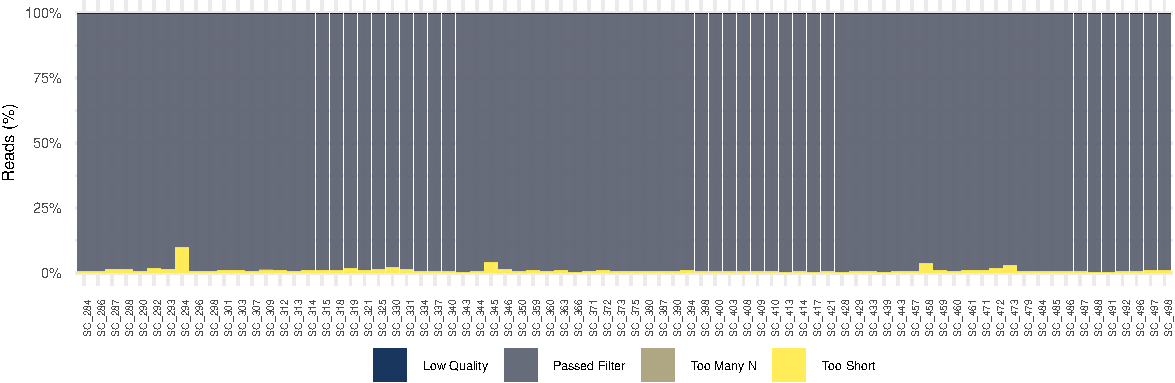
\includegraphics[keepaspectratio]{TFM_files/figure-pdf/fig-filter_reads-1.pdf}}

}

\caption{\label{fig-filter_reads}Fastp: Filtered Reads}

\end{figure}%

The adapters used in library construction, specifically the
\emph{Illumina Universal Adapter} type, are optimized for the
amplification and sequencing of diverse sample types. The adapter
trimming was highly effective, achieving a mean success rate of 99.38\%
(±0.35) with a range from 96.96\% to 99.62\%. (Table~\ref{tbl-metrics}).
In line with these findings, Figure~\ref{fig-adaptercontent} illustrates
the adapter content before and after processing with \emph{fastp}, where
the mean trimming percentage of 0.05 ± 0.06\% for scWAT samples
indicates that adapters were effectively removed from all samples. These
results confirm the efficiency of the preprocessing steps, ensuring that
high-quality reads were retained while effectively eliminating
low-quality sequences and adapters.

\begin{figure}[H]

\centering{

\pandocbounded{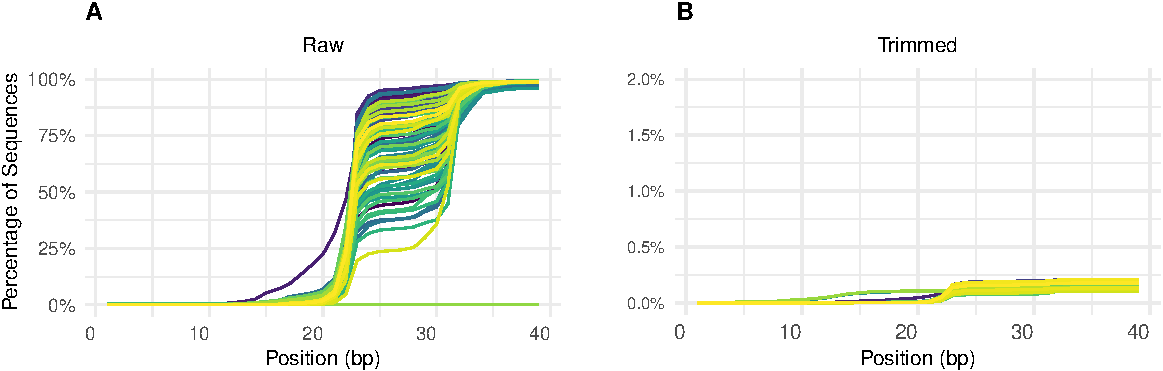
\includegraphics[keepaspectratio]{TFM_files/figure-pdf/fig-adaptercontent-1.pdf}}

}

\caption{\label{fig-adaptercontent}Adapters Content (\%) across all
bases before (A) and after (B) using \emph{fastp} (version 0.23.4)}

\end{figure}%

Figure~\ref{fig-fstqc_quality_control} shows the analysis of the mean
quality value of sequences across all bases, both before (\emph{A}) and
after (\emph{B}) processing with \emph{fastp}, it is evident from that
the sequences from all samples consistently fall within an acceptable
quality range, with mean Phred scores exceeding 30. This indicates a
high base-calling accuracy, with an error probability of less than
0.1\%, ensuring robust data integrity throughout the process.

However, there is a noticeable drop in quality towards the extremes of
the readings, particularly at position 31 bp. This decline can be
attributed to the effects of adapter trimming in smRNA-seq. Even though
adapters have been removed, if they were present at the end of the
sequence, their trimming may result in reduced quality for the
subsequent bases. Bases near the adapter might have lower quality,
leading to a set of bases that, while technically valid, originate from
a lower-quality region. Additionally, it is common in smRNA-seq to
encounter contaminants from various sources, such as rRNA or tRNA, which
introduce background noise and can further diminish the quality of the
readings obtained.

The Figure~\ref{fig-fstqc_quality_control} illustrates the metric of the
average quality value of each sequence across all samples. Before
processing with \emph{fastp} (\emph{C}), the Phred scores consistently
exceed 30, with most samples achieving scores around 35. This indicates
that the average sequence quality is optimal, ensuring high reliability
and low error rates. However, after trimming (\emph{D}) a slight
decrease in both Phred scores and read counts is observed. This
reduction in the number of reads is expected after strict preprocessing
with \emph{fastp}, especially if contaminated or low-quality reads were
present.

In Figure~\ref{fig-fstqc_quality_control} (\emph{E}), prior to trimming,
the GC content distribution does not follow a normal pattern. Multiple
peaks are observed, probably due to the presence of adapters, which
typically have a fixed GC content that generates specific peaks.
Additionally, since this is a \emph{small RNA-seq} experiment,
contamination from rRNA or tRNA is common, as these molecules often have
a different GC content compared to other small RNAs. After processing
with \emph{fastp} (\emph{F}), the GC content decreases, indicating that
most of these contaminant sequences have been removed, leaving of reads
with anomalies. This remaining may correspond to sequences that are
difficult to classify or contaminants that are not easily eliminated by
\emph{fastp}.

Additionally, no issues with the presence of ambiguous bases (Ns) are
detected in any of the samples before and after trimming.
Figure~\ref{fig-fstqc_quality_control} (\emph{G} and \emph{H}).

\begin{figure}[H]

\centering{

\pandocbounded{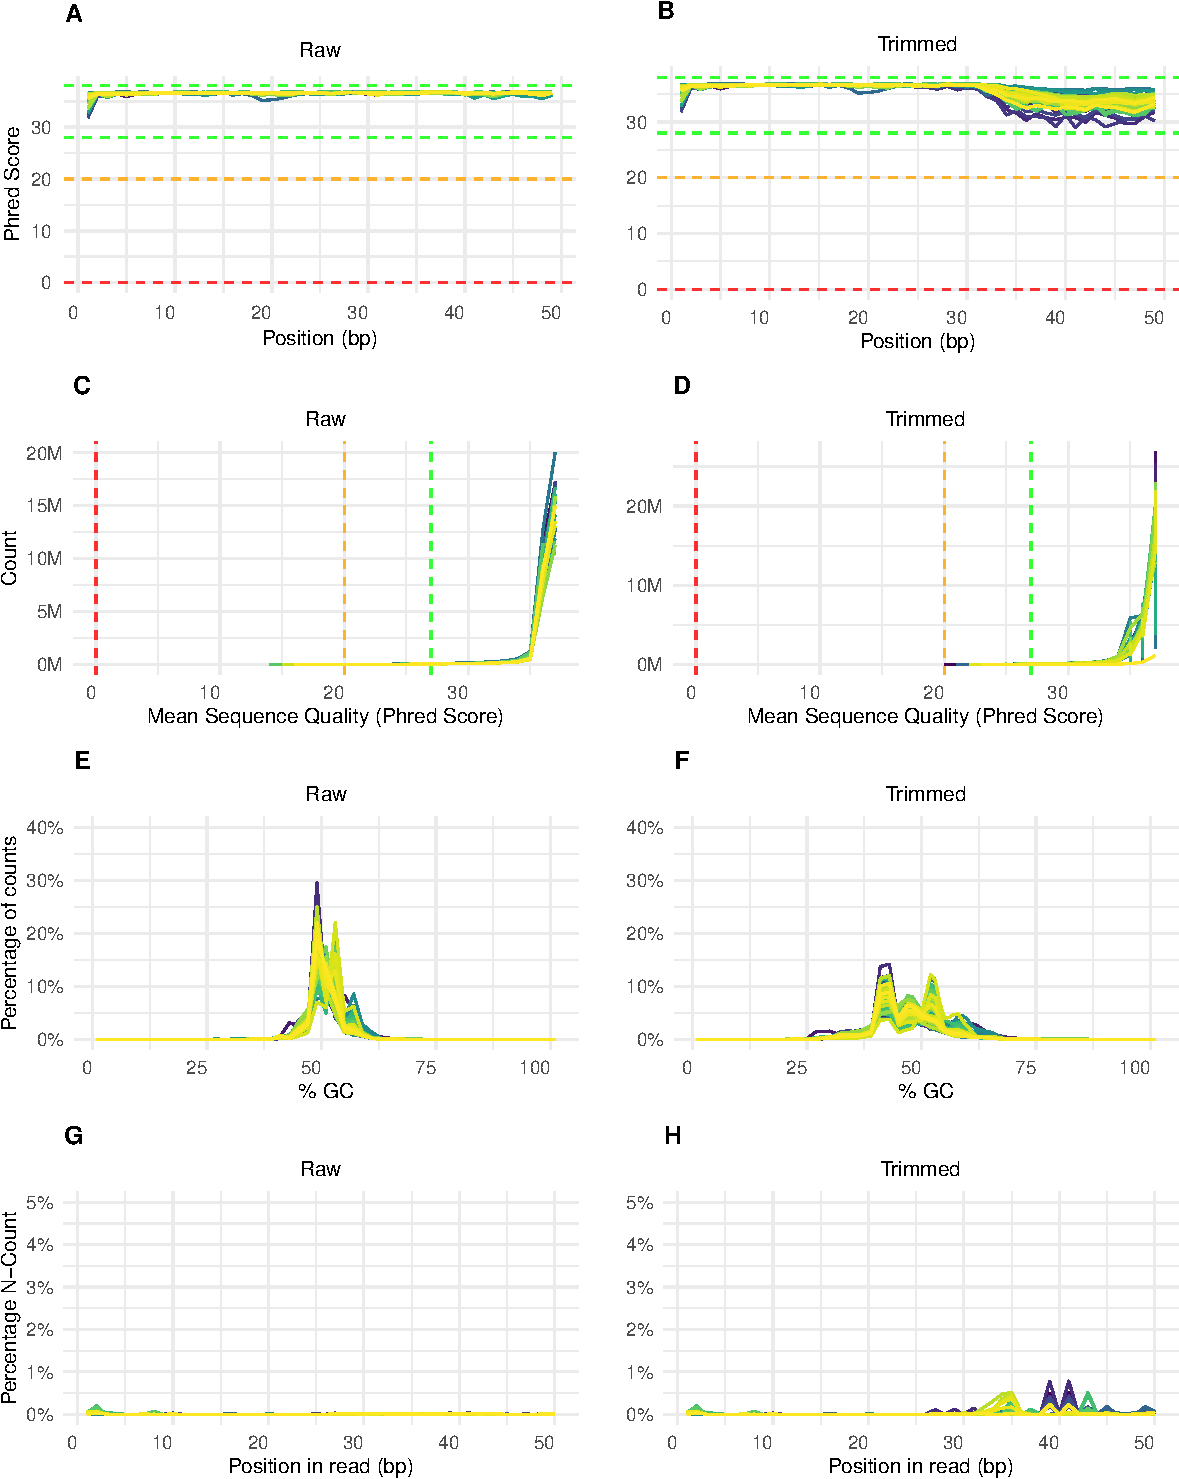
\includegraphics[keepaspectratio]{TFM_files/figure-pdf/fig-fstqc_quality_control-1.pdf}}

}

\caption{\label{fig-fstqc_quality_control}Quality Control Analysis.
\emph{A} and \emph{B}: Mean quality values of sequences across all bases
after (`Trimmed') and before (`Raw') using fastp (v0.23.4); \emph{C} and
\emph{D}: Per Sequence Quality Scores across all bases after (`Trimmed')
and before (`Raw') using fastp; \emph{E} and \emph{F}: Per Sequence GC
Content Raw after (`Trimmed') and before (`Raw') using fastp; \emph{G}
and \emph{H}: Read N content after (`Trimmed') and before (`Raw') using
fastp.}

\end{figure}%

However, the distribution of sequence lengths is irregular in the
samples Figure~\ref{fig-sld}. After trimming, the majority of sequences
cluster around a length of 20-25 nucleotides, although a smaller subset
of sequences with lengths between 29-32 nucleotides is also observed.
This indicates the presence of different types of small RNAs. Generally,
miRNAs are found in the range of 20-24 bp, with a peak at 22 bp
potentially indicating an abundant population of miRNAs. In contrast,
tRNAs can vary in length but are commonly found at lengths that may
include higher peaks, such as at 31 bp. This may reflect the presence of
tRNAs derived from the degradation of double-stranded RNA or
transposons.

\begin{figure}[H]

\centering{

\pandocbounded{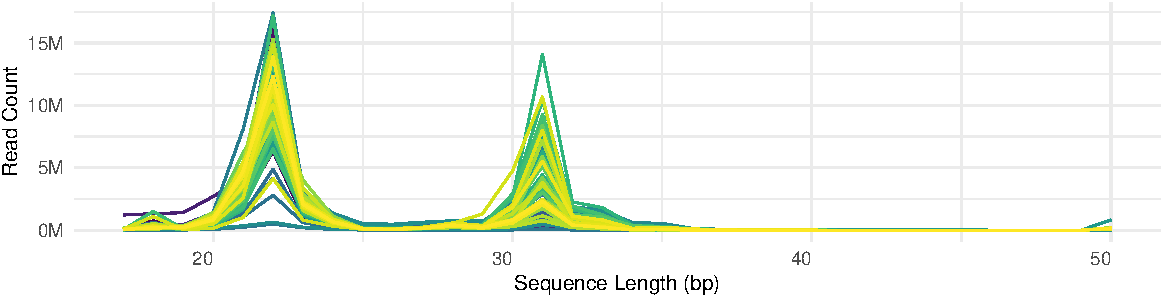
\includegraphics[keepaspectratio]{TFM_files/figure-pdf/fig-sld-1.pdf}}

}

\caption{\label{fig-sld}FastQC: Sequence Length Distribution}

\end{figure}%

In the Figure~\ref{fig-totalreads} shows the total number of reads
\emph{per} sample is around 25 million, both in Raw and Trimmed, with
means of 25.47 and 25.23 million, respectively. The interquartile ranges
(IQR) of these measurements are similar, approximately 4.2 million,
reflecting a high consistency among the samples.

Regarding duplicate reads, they dominate the data, with means of 25.10
million in Raw and 24.95 million in Trimmed, and an IQR of about 4.2
million in both conditions. This indicates that more than 90\% of the
sequences are duplicated, a high value but expected in sRNA-seq samples,
given the nature of the short reads of 20 to 24 nucleotides.

In contrast, unique reads are significantly less frequent, with means of
0.38 million in Raw and 0.28 million in Trimmed. The interquartile
ranges for these measurements are also low, around 0.13 million in Raw
and 0.10 million in Trim.

\begin{figure}[H]

\centering{

\pandocbounded{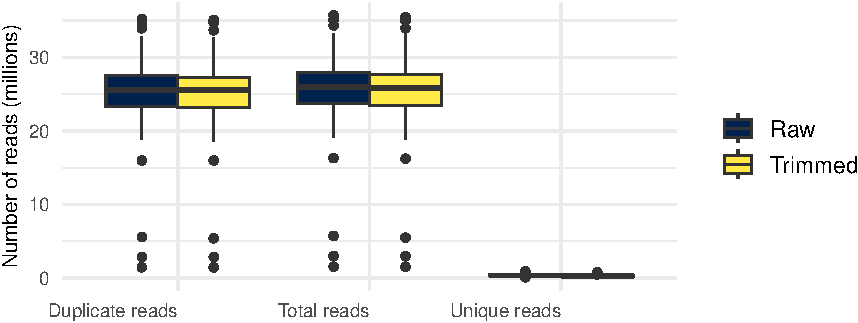
\includegraphics[keepaspectratio]{TFM_files/figure-pdf/fig-totalreads-1.pdf}}

}

\caption{\label{fig-totalreads}Number of reads from small RNA-seq. Total
reads before and after trimming of adapters}

\end{figure}%

\section{miRNA Quality Control}\label{mirna-quality-control}

The \emph{nf-core/smrnaseq} pipeline performs a quality analysis
specific to sRNA-seq data using \emph{miRTrace}. This analysis assesses
sequencing quality, identifies the presence of miRNA, and filters out
unwanted sequences such as tRNA, rRNA, or Illumina artifacts.
Additionally, it detects clade-specific miRNA profiles based on a
comprehensive catalog of previously identified miRNA families.

In the annotation step Figure~\ref{fig-mirtrace_RNA_Categories}, the
mapped reads against reference databases revealed that a mean of 65.06\%
of analyzed sequences per sample corresponded to miRNA precursors, with
a range of 22.51\% to 91.77\%. Other categories included 21.16\% tRNA
sequences, 9.16\% unknown sequences, 4.55\% rRNA sequences, and 0.05\%
artifacts.

\begin{figure}[H]

\centering{

\pandocbounded{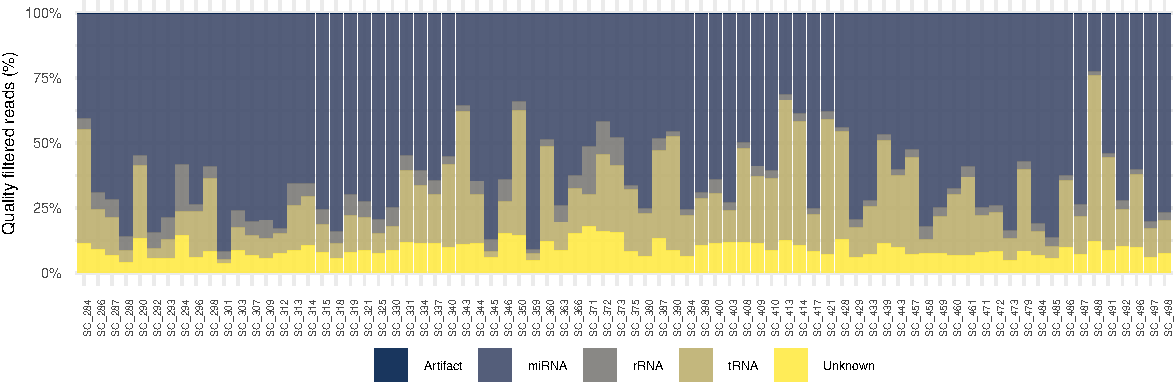
\includegraphics[keepaspectratio]{TFM_files/figure-pdf/fig-mirtrace_RNA_Categories-1.pdf}}

}

\caption{\label{fig-mirtrace_RNA_Categories}\emph{miRTrace} (v1.0.1)
Analysis: RNA Categories}

\end{figure}%

During the contamination assessment step
Figure~\ref{fig-mirtrace_Contamination_Check}, mapping miRNA precursor
sequences against the clade-specific miRNA catalog showed that a mean of
94.14\% of analyzed sequences belonged to the human category, with a
range of 67.21\% to 99.94\%. Minor contributions from other clades, such
as Rodentia (2.07\%), Dicots (2.73\%), Insects (0.58\%), and Monocots
(0.38\%), were detected at low proportions. These identifications could
result from contamination, such as incorrect index assignment during
sample demultiplexing.

\begin{figure}[H]

\centering{

\pandocbounded{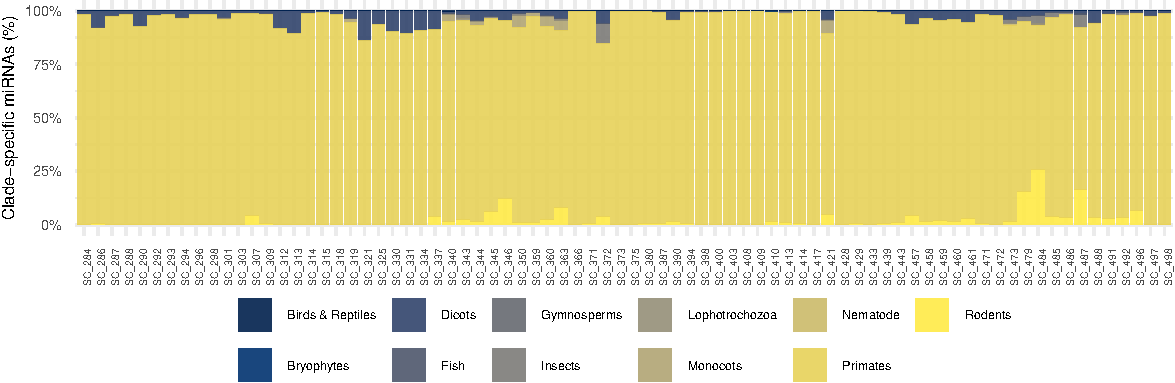
\includegraphics[keepaspectratio]{TFM_files/figure-pdf/fig-mirtrace_Contamination_Check-1.pdf}}

}

\caption{\label{fig-mirtrace_Contamination_Check}\emph{miRTrace}
(v1.0.1) Analysis: Contamination Check}

\end{figure}%

\section{miRNA Quantification}\label{mirna-quantification}

In this step of the \emph{nf-core/smrnaseq pipeline}, the alignment of
reads is conducted sequentially against databases of mature miRNAs,
precursor miRNAs, and a combined database of both. These alignments
enable the identification and quantification of miRNAs. The statistics
obtained for mature miRNAs, precursor miRNAs, and the combination of
both against the reference genome are presented in
Table~\ref{tbl-samtools_overall}. On average, 52.07\% of the mature
miRNAs were mapped, with a range between 17.72\% and 79.75\%.

For precursor miRNAs, an average of 32.33\% of sequences were
identified, ranging from 6.31\% to 68.83\%. Subsequently, the reads of
mature and precursor miRNAs were aligned against a reference genome, not
for miRNA identification and quantification but as a quality control for
the sequences. In this regard, the mean percentage of aligned reads was
around 43\% of the total reads. Across the sample set, minimum values of
10.28\% and maximum values of 73.31\% were observed. For more details,
the metrics for each sample can be found in
\url{https://github.com/joshoandres13/miRNAs}.

\begingroup\fontsize{11}{13}\selectfont

\begin{longtable}[t]{lrrrrr}

\caption{\label{tbl-samtools_overall}Descriptive statistics of alignment
with samtools of all samples. \emph{TM}: Mean of Total Mapped (reads);
\emph{TU}: Mean of Total Unmapped (reads): \emph{Mean M}: Mean Mapped
(\%); \emph{Max M}: Max Mapped (\%); \emph{Min M}: Min Mapped (\%)}

\tabularnewline

\toprule
\textbf{Group} & \textbf{TM} & \textbf{TU} & \textbf{Mean M} & \textbf{Max M} & \textbf{Min M}\\
\midrule
mature & 13166950 & 12194855 & 52.07 & 79.75 & 17.72\\
mature\_hairpin & 3644435 & 8836242 & 32.33 & 68.83 & 6.31\\
mature\_hairpin\_genome & 4334118 & 4565712 & 43.87 & 73.31 & 10.28\\
\bottomrule

\end{longtable}

\endgroup{}

\section{IsomiR Annotation}\label{isomir-annotation}

\emph{Mirtop} (v0.4.28) was used for the annotation of miRNAs and
isomiRs. In Figure~\ref{fig-mirtop_mean_isomir_read_counts}, the
\emph{mean isomiR read counts} are presented, which refer to an average
calculation that helps to describe how the reads of isomiRs are
distributed within a dataset. Among the annotated isomiR sequences per
sample, the \emph{reference miRNA} accounts for 96.51\%, with ranges
varying from 88.70\% to 98.13\%. On the other hand, the distributions of
isomiR variants are as follows: \emph{3' Isoform} (1.36\%), \emph{3'
Addition} (1.23\%), \emph{5' Isoform} (0.64\%), \emph{SNVs in the
Central Offset Region} (0.05\%), \emph{SNVs in the Central Region}
(0.06\%), \emph{Supported SNVs in the Central Region} (0.05\%), and
\emph{SNV in Seed Region} (0.05\%), all of which are below 1.40\%.

\begin{figure}[H]

\centering{

\pandocbounded{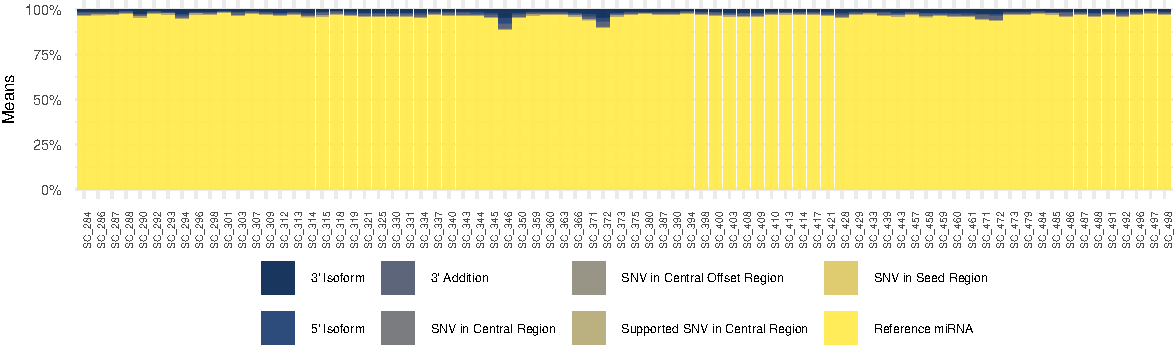
\includegraphics[keepaspectratio]{TFM_files/figure-pdf/fig-mirtop_mean_isomir_read_counts-1.pdf}}

}

\caption{\label{fig-mirtop_mean_isomir_read_counts}Annotation of miRNAs
and isomiRs with \emph{mirtop} (v0.4.28): Mean isomiR read counts}

\end{figure}%

\section{Differential expression
analysis}\label{differential-expression-analysis}

Differential expression analysis is a bioinformatics and statistical
technique used to identify genes, proteins, or other biomolecules that
exhibit significant differences in expression levels between two or more
biological conditions. For this analysis, the sequences of miRNAs of
reference were used, as annotated in the previous analysis.

Under the hood of \emph{DESeq2}, we applied the \emph{regularized
logarithm} (\emph{rlog}) transformation for normalization, which
incorporates a prior on the sample
differences\textsuperscript{{[}148{]}}. This step is crucial because the
standard logarithmic transformation can be sensitive to low expression
values, whereas \emph{rlog} addresses this issue by introducing
regularization that helps stabilize variability between samples. This
method facilitates seamless integration into subsequent analyses, as
demonstrated in Figure~\ref{fig-heatmap}, which shows a total of 374
miRNAs were found to be expressed differentially in the overall cohort
when patients (samples) were categorized by sex and steatosis.

Since we were primarily interested in the transcriptional changes that
may precede the initiation of the steatosis process, we focused on
contrasting individuals across different levels of steatosis. In this
experimental scenario, the goal is to identify miRNAs that are expressed
differentially at various levels of steatosis. In our differential
expression analysis using \emph{DESeq2} with the LRT model, we initially
identified 169 miRNAs as upregulated and 205 downregulated in the
subcutaneous white adipose tissue (scWAT) of individuals according their
steatosis degree. Comparing these four groups and applying a false
discovery rate (FDR) cutoff of less than 0.05, the number of
statistically siginificant differentially expressed miRNAs was greatly
reduced to 2 (Figure~\ref{fig-volcan}). Of these, we found
\emph{hsa-miR-372-3p} is upregulated and \emph{hsa-miR-144-3p} is
downregulated (Table~\ref{tbl-mirnas_selected}).

\begingroup\fontsize{11}{13}\selectfont

\begin{longtable}[t]{lrlr}

\caption{\label{tbl-mirnas_selected}Differentially expressed miRNAs in
subcutaneous white adipose tissue (scWAT). \emph{FDR} : False Discovery
Rate}

\tabularnewline

\toprule
\textbf{} & \textbf{log2FoldChange} & \textbf{pvalue} & \textbf{FDR}\\
\midrule
hsa-miR-144-3p & -3.319 & p< 0.0002 & 0.04\\
hsa-miR-372-3p & 1.085 & p< 0.0002 & 0.04\\
\bottomrule

\end{longtable}

\endgroup{}

\begin{figure}[H]

\centering{

\pandocbounded{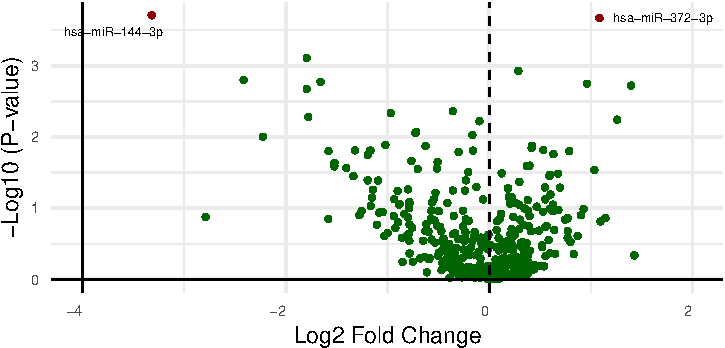
\includegraphics[keepaspectratio]{TFM_files/figure-pdf/fig-volcan-1.pdf}}

}

\caption{\label{fig-volcan}Plot showing differentially expressed miRNAs
(red) in subcutaneous white adipose tissue (scWAT) according to the four
groups of steatosis}

\end{figure}%

\clearpage

\begin{figure}[H]

\centering{

\pandocbounded{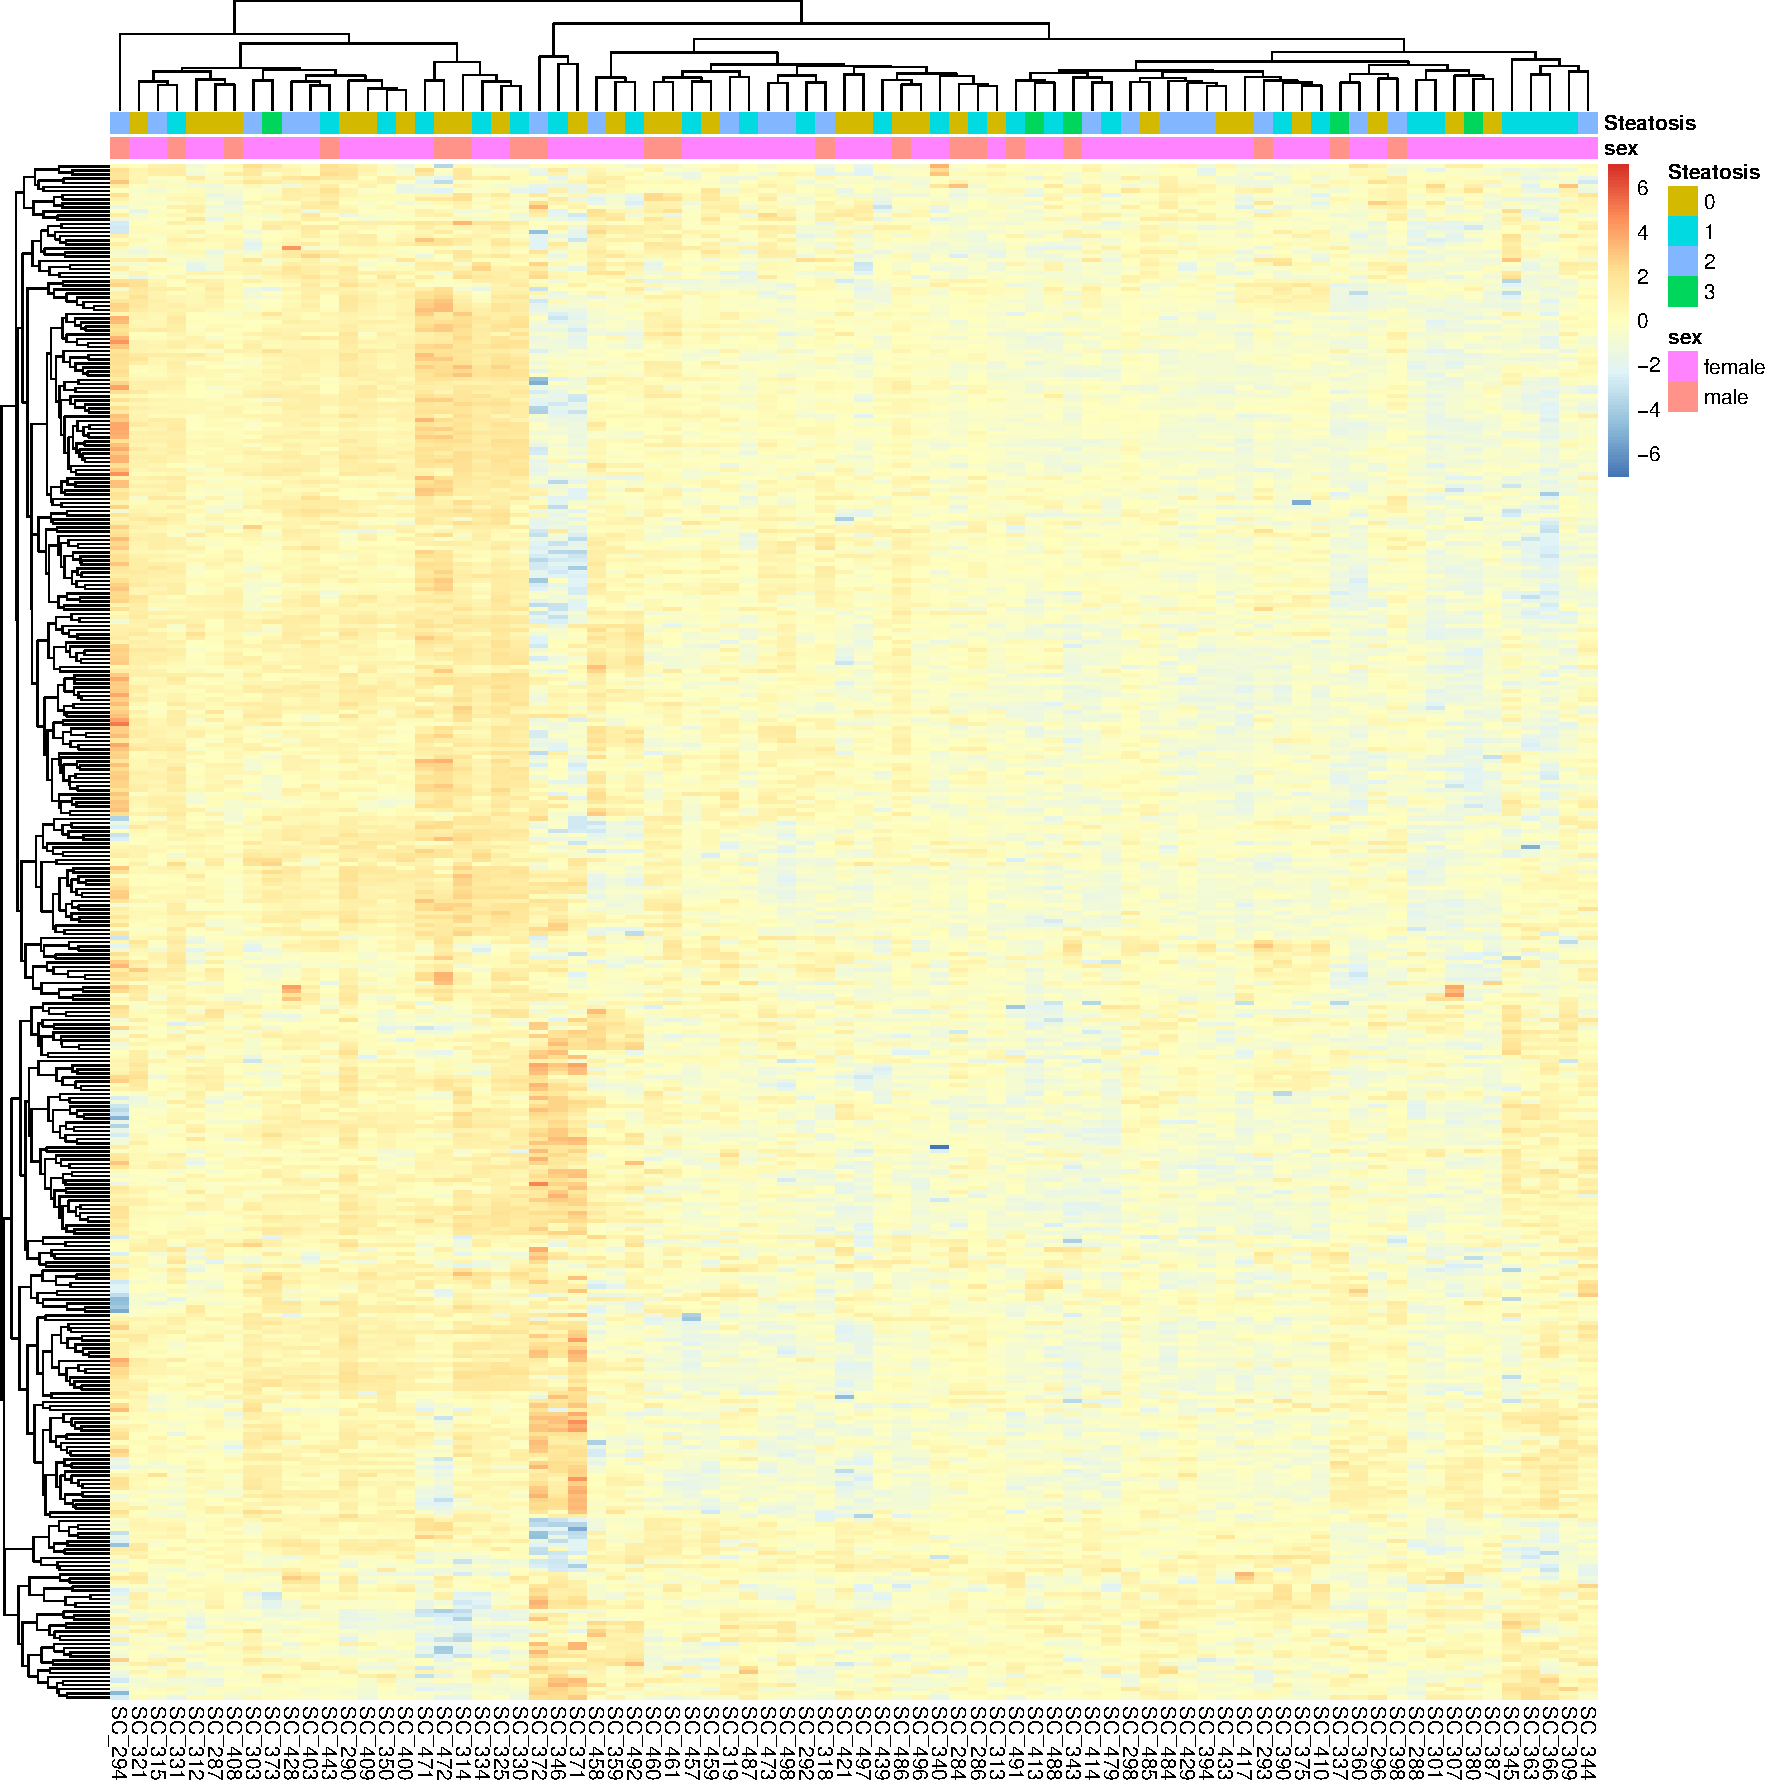
\includegraphics[keepaspectratio]{TFM_files/figure-pdf/fig-heatmap-1.pdf}}

}

\caption{\label{fig-heatmap}The heatmap illustrates the expression of
374 individual miRNA sequences across the analyzed samples. In this
visualization, shades of red indicate increased miRNA expression,
whereas shades of blue denote reduced or absent miRNA expression.
Although a substantial number of miRNAs were identified, no distinct
grouping patterns emerged among the analyzed samples, suggesting
heterogeneity in miRNA expression profiles across the dataset.}

\end{figure}%

\clearpage

Following their identification, we further analyzed the expression
patterns of these two differentially expressed miRNAs by representing
their normalized counts in boxplots across the four steatosis groups
Figure~\ref{fig-mirnasselected}.The boxplots highlight the consistency
of expression changes across groups, reinforcing the relevance of these
miRNAs in the context of steatosis severity. The miRNA
\emph{hsa-miR-144-3p} pattern of expression a significant decrease in
expression as steatosis levels increase, whereas \emph{hsa-miR-372-3p}
exhibits a trend of progressively higher expression across the varying
levels of steatosis.

Despite observing a trend of increasing expression of
\emph{hsa-miR-372-3p} with rising levels of steatosis, the results from
the Kruskal-Wallis test did not achieve statistical significance
(\emph{p}= 0.28) when comparing the different states of steatosis. This
suggests that, while there may be a tendency towards increased
expression of the miRNA with the progression of steatosis, a larger
sample size or an alternative approach is needed to draw firmer
conclusions about its role in the progression of the disease.

\begin{figure}[H]

\centering{

\pandocbounded{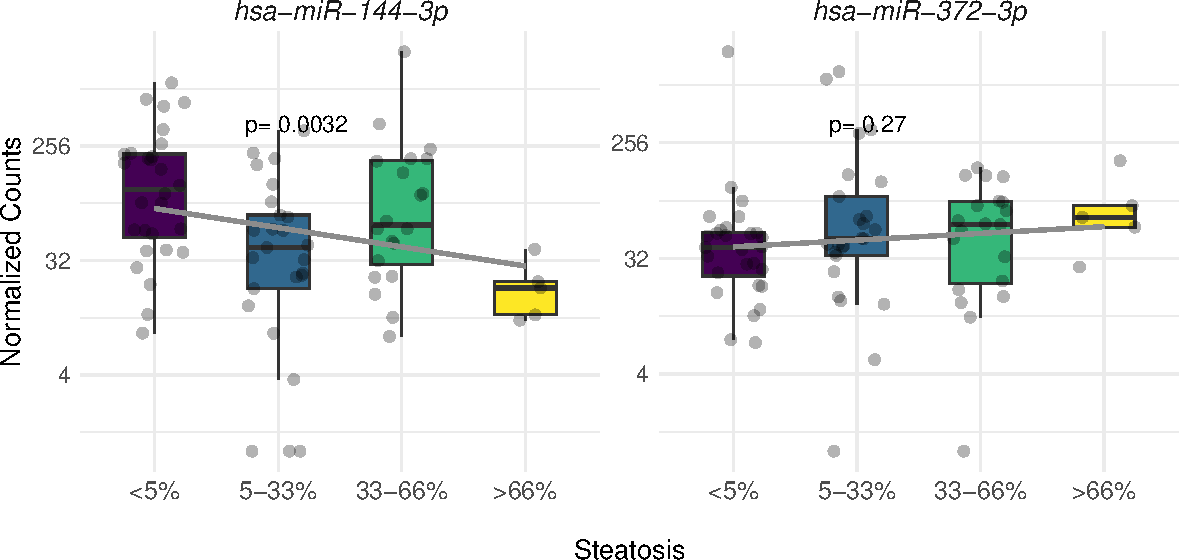
\includegraphics[keepaspectratio]{TFM_files/figure-pdf/fig-mirnasselected-1.pdf}}

}

\caption{\label{fig-mirnasselected}Boxplots of the differentially
expressed miRNAs in subcutaneous white adipose tissue (scWAT) according
to the four groups of steatosis. Each box represents the interquartile
range (IQR) of the normalized counts, with the line inside the box
indicating the median. The whiskers extend to show the range of the
data, excluding outliers, which are displayed as individual points.
\emph{p}: p-value fot the Kruskal--Wallis test for the comparison
between groups.}

\end{figure}%

\section{Target mRNA Selection and
Validation}\label{target-mrna-selection-and-validation}

\subsection{\texorpdfstring{\emph{hsa-miR-372-3p}}{hsa-miR-372-3p}}\label{hsa-mir-372-3p}

Potential target genes of the selected miRNAs were identified using the
\emph{multiMiR} package. This analysis included only validated
interaction data, ensuring the biological relevance of the identified
mRNAs. A subsequent filtering process was applied to select targets
based on the type of experimental validation (e.g., luciferase assays,
Western blot, or qRT-PCR) and functional support. As shown in
Table~\ref{tbl-hsa-miR-372-3p}, 24 target genes were identified after
filtering.

\begingroup\fontsize{11}{13}\selectfont

\begin{longtable}[t]{ll}

\caption{\label{tbl-hsa-miR-372-3p}Selected interactions after filtering
by database, experiment type (including luciferase assays, Western blot,
or qRT-PCR), functional support (Functional MTI) and validated type for
\emph{hsa-miR-372-3p}.}

\tabularnewline

\toprule
\textbf{Gene} & \textbf{Ensembl Identifier}\\
\midrule
LATS2 & ENSG00000150457\\
TGFBR2 & ENSG00000163513\\
NFIB & ENSG00000147862\\
CDKN1A & ENSG00000124762\\
VEGFA & ENSG00000112715\\
\addlinespace
TNFAIP1 & ENSG00000109079\\
TRPS1 & ENSG00000104447\\
MBNL2 & ENSG00000139793\\
RHOC & ENSG00000155366\\
NR4A2 & ENSG00000153234\\
\addlinespace
ERBB4 & ENSG00000178568\\
CDK2 & ENSG00000123374\\
LEFTY1 & ENSG00000243709\\
BTG1 & ENSG00000133639\\
WEE1 & ENSG00000166483\\
\addlinespace
CCNA1 & ENSG00000133101\\
DKK1 & ENSG00000107984\\
PHLPP2 & ENSG00000040199\\
ATAD2 & ENSG00000156802\\
ADAMTS9 & ENSG00000163638\\
\addlinespace
CADM2 & ENSG00000175161\\
ZBTB7A & ENSG00000178951\\
TXNIP & ENSG00000265972\\
KLF13 & ENSG00000275746\\
\bottomrule

\end{longtable}

\endgroup{}

The target genes identified through \emph{multiMiR} were subjected to
functional enrichment analysis using KEGG (Kyoto Encyclopedia of Genes
and Genomes) pathways\textsuperscript{{[}144{]}}. The KEGG pathway
enrichment analysis identified five significantly enriched pathways (p
\textless{} 0.05) (Figure~\ref{fig-enrichment_hsamiR_372_3p}). The most
prominent pathways include:

\begin{itemize}
\tightlist
\item
  \emph{Cellular senescence} (KEGG ID: hsa04218): associated with
  cellular aging and the permanent arrest of the cell cycle in response
  to genetic damage, oxidative stress, or oncogenic signals.
\item
  \emph{Cell cycle} (KEGG ID: hsa04110): involved in the regulation and
  progression of the cell cycle, including critical checkpoints that
  ensure the fidelity of cell division.
\item
  \emph{Hepatitis B} (KEGG ID: hsa05161): related to infection by the
  hepatitis B virus and the inflammatory and carcinogenic processes it
  can trigger in the liver.
\item
  \emph{PI3K-Akt signaling pathway} (KEGG ID: hsa04151): a key pathway
  regulating cellular processes such as proliferation, survival, and
  metabolism, frequently deregulated in cancer. This pathway is related
  with insuline resistence.
\item
  \emph{Pancreatic cancer} (KEGG ID: hsa05212): associated with
  molecular and cellular alterations characteristic of this cancer type,
  including aberrant signaling and apoptosis resistance.
\end{itemize}

These pathways are primarily linked to essential processes such as
\emph{cell cycle regulation}, \emph{intracellular signaling in cancer},
and \emph{cellular responses to damage and infection}.

\begin{figure}[H]

\centering{

\pandocbounded{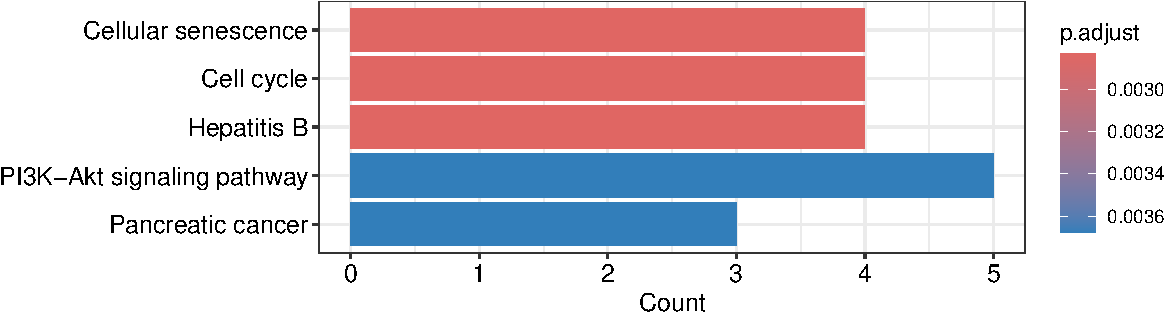
\includegraphics[keepaspectratio]{TFM_files/figure-pdf/fig-enrichment_hsamiR_372_3p-1.pdf}}

}

\caption{\label{fig-enrichment_hsamiR_372_3p}Top 5 Significant KEGG
Pathways of \emph{hsa-miR-372-3p}}

\end{figure}%

\subsection{\texorpdfstring{\emph{hsa-miR-144-3p}}{hsa-miR-144-3p}}\label{hsa-mir-144-3p}

Table~\ref{tbl-hsa-miR-144-3p} shows 22 target genes were identified for
\emph{hsa-miR-372-3p}, filtered by validated interactions and
experimental evidence.

\begingroup\fontsize{11}{13}\selectfont

\begin{longtable}[t]{ll}

\caption{\label{tbl-hsa-miR-144-3p}Selected interactions after filtering
by database, experiment type (including luciferase assays, Western blot,
or qRT-PCR), functional support (Functional MTI) and validated type for
\emph{hsa-miR-144-3p}.}

\tabularnewline

\toprule
\textbf{Gene} & \textbf{Ensembl Identifier}\\
\midrule
NOTCH1 & ENSG00000148400\\
PLAG1 & ENSG00000181690\\
ZEB1 & ENSG00000148516\\
ZEB2 & ENSG00000169554\\
IRS1 & ENSG00000169047\\
\addlinespace
MAP3K8 & ENSG00000107968\\
EZH2 & ENSG00000106462\\
APP & ENSG00000142192\\
PTGS2 & ENSG00000073756\\
MET & ENSG00000105976\\
\addlinespace
ETS1 & ENSG00000134954\\
TGFB1 & ENSG00000105329\\
CFTR & ENSG00000001626\\
FGG & ENSG00000171557\\
MTOR & ENSG00000198793\\
\addlinespace
SMAD4 & ENSG00000141646\\
NFE2L2 & ENSG00000116044\\
PBX3 & ENSG00000167081\\
TTN & ENSG00000155657\\
TUG1 & ENSG00000253352\\
\addlinespace
PTEN & ENSG00000284792\\
XIST & ENSG00000229807\\
\bottomrule

\end{longtable}

\endgroup{}

The target genes identified through \emph{multiMiR} were subjected to
functional enrichment analysis using KEGG where five significantly
enriched pathways (p \textless{} 0.05)
(Figure~\ref{fig-enrichment_hsamiR_144_3p}). The most prominent pathways
include:

\begin{itemize}
\tightlist
\item
  \emph{MicroRNAs in cancer} (KEGG ID: hsa05206): Highlighting the role
  of miRNAs in the regulation of gene expression, particularly in
  pathways associated with tumorigenesis and cancer progression.\\
\item
  \emph{Hepatocellular carcinoma} (KEGG ID: hsa05225): Specifically
  linked to liver cancer and the molecular mechanisms underlying its
  development and progression.\\
\item
  \emph{FoxO signaling pathway} (KEGG ID: hsa04068): A critical pathway
  regulating oxidative stress response, apoptosis, and metabolism, which
  plays a significant role in cancer and aging.\\
\item
  \emph{Gastric cancer} (KEGG ID: hsa05226): Associated with molecular
  and cellular alterations characteristic of gastric tumorigenesis.\\
\item
  \emph{Cellular senescence} (KEGG ID: hsa04218): Related to aging and
  the permanent arrest of the cell cycle due to stress signals or
  damage.
\end{itemize}

\begin{figure}[H]

\centering{

\pandocbounded{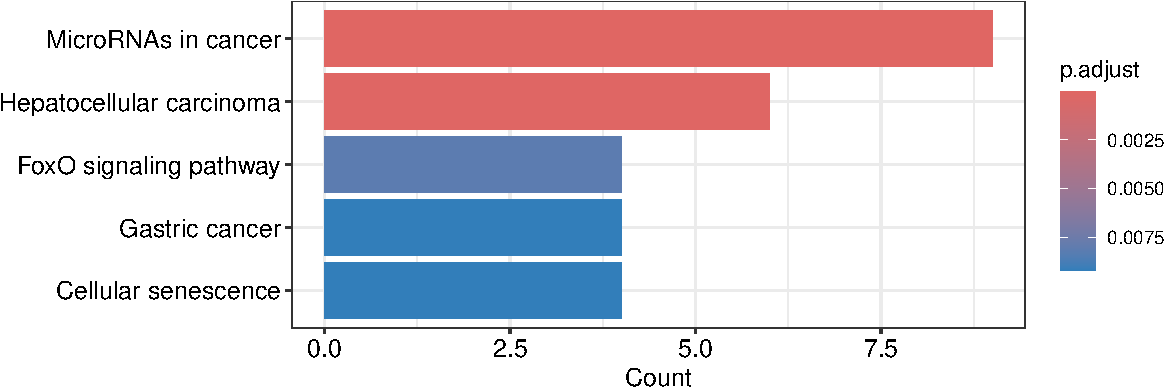
\includegraphics[keepaspectratio]{TFM_files/figure-pdf/fig-enrichment_hsamiR_144_3p-1.pdf}}

}

\caption{\label{fig-enrichment_hsamiR_144_3p}Top 5 Significant KEGG
Pathways of \emph{hsa-miR-144-3p}}

\end{figure}%

These pathways reflect key biological processes, including
tumorigenesis, stress response, and cell cycle regulation, underscoring
the importance of miRNAs in these mechanisms. The findings provide
valuable insights into potential molecular interactions and pathways
relevant to the studied system.

\section{\texorpdfstring{The \emph{hsa-miR-372-3p} and
\emph{hsa-miR-144-3p} in an in vitro model of lipid
steatosis.}{The hsa-miR-372-3p and hsa-miR-144-3p in an in vitro model of lipid steatosis.}}\label{the-hsa-mir-372-3p-and-hsa-mir-144-3p-in-an-in-vitro-model-of-lipid-steatosis.}

The gene expression was evaluated in HepG2 cells transfected for 24
hours and then treated with Oleic Acid (OA) for an additional 24 hours
to assess the impact of single miRNA in a cell model mimicking hepatic
steatosis. Specifically, we investigated the relative expression of
\emph{PPARG} (Peroxisome Proliferator Activated Receptor Gamma), a key
regulator of adipogenesis and insulin sensitivity; \emph{PNPLA2}
(Patatin Like Phospholipase Domain Containing 2), which encodes the
Adipose Triglyceride Lipase (\emph{ATGL}) involved in triglyceride
breakdown; \emph{DGAT2} (Diacylglycerol O-Acyltransferase 2), a critical
enzyme for triglyceride synthesis; \emph{FAS} (Fas Cell Surface Death
Receptor), a mediator of apoptosis and cellular stress; and \emph{ACACA}
(Acetyl-CoA Carboxylase Alpha), the rate-limiting enzyme in \emph{de
novo} fatty acid synthesis. These genes play pivotal roles in lipid
metabolism and, to a lesser extent, glucose metabolism, making them
relevant targets for understanding the molecular mechanisms underlying
hepatic steatosis.

The synthetic \emph{miR-372} mimic significantly downregulated the mRNA
expression of the gene \emph{ACAC} (-91.40\% ± 3.39; p \textless{} 0.05)
in OA-treated HepG2 cells. A similar, although not statistically
significant, decrease was observed in the mRNA levels of \emph{FAS}
(-90.50\% ± 4.30; p \textless{} 0.093), suggesting a trend towards
reduced expression. In contrast, the mRNA levels of \emph{DGAT2}
(-73.7\% ± 6.70; p = 0.462) and \emph{PNPLA2} (-55.10\% ± 19.56; p =
0.243) did not show significant changes. Notably, the mRNA levels of
\emph{PPARG} remained unchanged compared to the negative control cells
(Figure~\ref{fig-rge_mir372}).

\begin{figure}[H]

\centering{

\pandocbounded{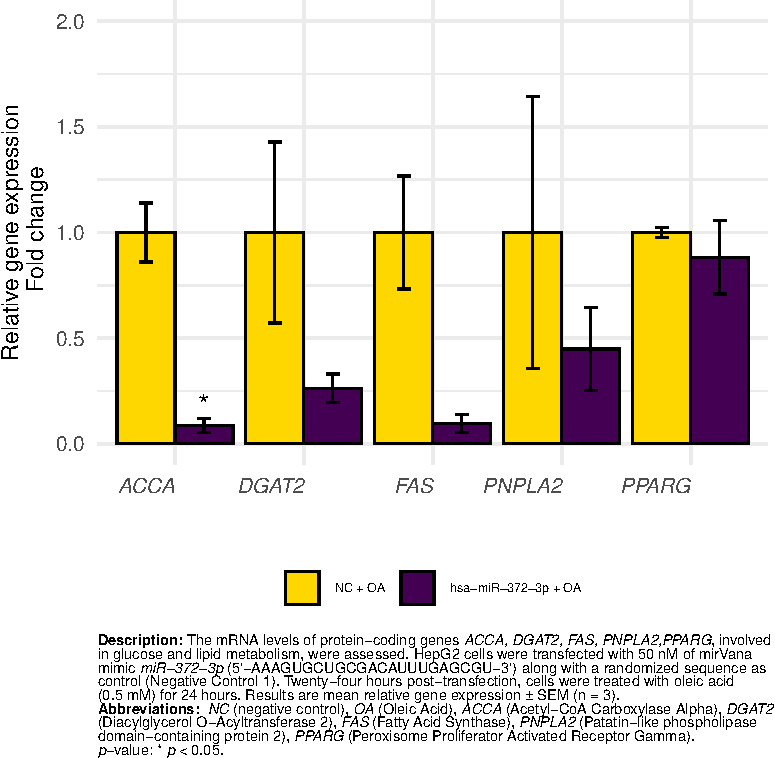
\includegraphics[keepaspectratio]{TFM_files/figure-pdf/fig-rge_mir372-1.pdf}}

}

\caption{\label{fig-rge_mir372}Gene expression analysis of HepG2 cells
transfected with \emph{miR-372-3p} mimic and negative control (scramble
sequence) were treated with oleic acid to mimic in vitro hepatic
steatosis.}

\end{figure}%

On the other hand, inhibition of \emph{hsa-miR-144-3p} upregulated the
expression of the genes involved in lipid metabolism.. The relative gene
expression levels of the evaluated targets in HepG2 cells transfected
and treated with Oleic Acid (OA) were as follows: \emph{ACACA} (96.80\%
± 53.79; p = 0.186), \emph{FAS} (135\% ± 160.34; p = 0.429),
\emph{DGAT2} (32.74\% ± 24.13; p = 0.128), \emph{PNPLA2} (48.83\% ±
14.32; p = 0.140), and \emph{PPARG} (64.09\% ± 41.25; p = 0.239)
(Figure~\ref{fig-rge_mir372}). Although the expression levels varied
across genes, none of these changes were statistically significant (p
\textgreater{} 0.05). These findings suggest that the regulatory effect
of \emph{hsa-miR-144-3p} on these genes may be limited under the
experimental conditions employed.

\begin{figure}[H]

\centering{

\pandocbounded{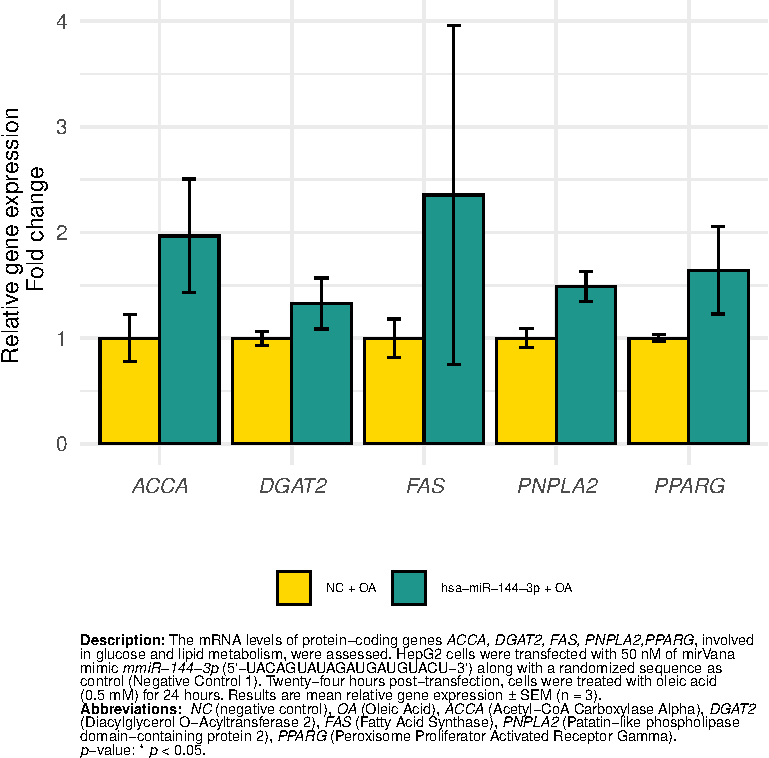
\includegraphics[keepaspectratio]{TFM_files/figure-pdf/fig-rge_mir144-1.pdf}}

}

\caption{\label{fig-rge_mir144}Gene expression analysis of HepG2 cells
transfected with \emph{miR-144-3p} inhibitor and negative control
(scramble sequence) were treated with oleic acid to mimic in vitro
hepatic steatosis.}

\end{figure}%

\chapter{Discussion}\label{discussion}

This study presents new insights about the role of miRNAs from
subcutaneous adipose tissue in regulating metabolic processes related to
hepatic steatosis. Through the analysis of smRNA-seq, differential
miRNAs linked to key metabolic pathways were identified that may play a
role in liver fat accumulation and the progression of hepatic steatosis
in obese individuals. These findings address a critical gap in
understanding the role of miRNAs in adipose-liver metabolic crosstalk,
which has implications for targeted interventions in hepatic steatosis
and bring new avenues for their eventual use as biomakers.

Previous studies have extensively investigated the role of miRNAs as
potential biomarkers in MASLD and HCC, highlighting their regulatory
functions in disease development and progression at various
levels\textsuperscript{{[}119,149--152{]}}. Among these,
\emph{miRNA-34a} and \emph{miRNA-122} stand out as the most extensively
studied in MASLD patients\textsuperscript{{[}153,154{]}}. Furthermore,
other miRNAs have also been associated with MASLD, as shown in studies
by Liu et al., Gjorgjieva et al., and Szabo et
al.\textsuperscript{{[}73,153,155{]}}. Notably, \emph{miR-122-5p},
\emph{miR-151a-3p}, \emph{miR-126-5p}, and \emph{miR-21-5p} have been
proposed as predictive biomarkers for assessing MASLD at different
stages of dietary interventions\textsuperscript{{[}156,157{]}}.

Beyond MASLD, miRNAs have been widely associated with other metabolic
dysfunction-related disorders, including diabetes and
T2DM\textsuperscript{{[}72{]}}. For instance, tissue and circulating
miRNAs have been identified as biomarkers of response to obesity
treatment strategies in diseases such as
diabetes\textsuperscript{{[}158{]}}.

Lastly, specific miRNAs have also been proposed as biomarkers in liver
steatosis. Early studies identified miRNAs promising indicators of liver
dysfunction\textsuperscript{{[}159{]}}, while others analyzed their
expression in human omental and subcutaneous adipose
tissue\textsuperscript{{[}152{]}}. These findings emphasize the
relevance of miRNAs not only in MASLD but also in broader contexts of
metabolic and hepatic diseases.

In contrast to these previous studies, to our knowledge, our study is
the first to identify differentially expressed miRNAs in subcutaneous
with sm-RNA seq in scWAT from 78 obese individuals within the FATe
cohort, which encompasses different scales of hepatic steatosis, and
being validated \emph{in vitro} through a model of human hepatocyte
cells. Building on these insights, we specifically focused on
identifying differentially expressed miRNAs associated with hepatic
steatosis in subcutaneous adipose tissue to understand the direct
relationship between hepatic steatosis and the expression of specific
miRNAs in subcutaneous adipose tissue.

Understanding the expression patterns of miRNAs across different tissues
is essential for gaining deeper insights into both normal development
and disease progression in these tissues\textsuperscript{{[}160{]}}.
Adipose tissue--liver crosstalk has been proposed to occur during MASLD,
with factors originating from both adipose tissue and the liver
identified as potential drivers of disease progression. Among these
factors, miRNAs stand out, as their dysregulation in metabolic
disturbances suggests a direct involvement in such
conditions\textsuperscript{{[}161{]}}. This highlights that alterations
in miRNA signaling may play a role in obesity, metabolic syndrome, or
MASLD.

\emph{hsa-miR-372-3p} has been identified as a potent miRNA associated
with tumorigenesis\textsuperscript{{[}162{]}}. It has been shown to
promote tumor formation in testicular germ cell
tumors\textsuperscript{{[}163,164{]}}, lung
cancer\textsuperscript{{[}165{]}}, parathyroid
carcinoma\textsuperscript{{[}162{]}}, and
osteosarcoma\textsuperscript{{[}166{]}}. However, recent studies have
highlighted the role of \emph{hsa-miR-372-3p} in the context of MASH.
Specifically, metabolic dysregulation leads to an increased expression
of adipocyte enhancer binding protein 1 (\emph{AEBP1}) in liver
cells\textsuperscript{{[}167{]}}. Its emerging role in the formation of
collagen-rich tissues and the development of tissue fibrosis is also
significant in the context of MASH\textsuperscript{{[}168{]}}. Also,
\emph{AEBP1} is a key component of a group of genes specifically
dysregulated in the fibrotic processes associated with
MASH\textsuperscript{{[}72{]}}. Notably, the levels of
\emph{hsa-miR-372-3p} is found to be lower in patients with MASH and
advanced fibrosis, where this miRNA interact functionally with
\emph{AEBP1} to reduce its expression. This suggests that the
dysregulation of this miRNA may contribute to the progression of hepatic
steatosis and its associated complications, further linking
\emph{hsa-miR-372-3p} to the metabolic dysregulation observed in
MASH\textsuperscript{{[}168{]}}.

Through transcriptomic and pathway analysis, we predicted additional
pathways already experimentally validated in which \emph{hsa-miR-372-3p}
is implicated. These pathways support its role in tumorigenesis, they
also suggest a broader implication of \emph{hsa-miR-372-3p} in metabolic
disorders, particularly in processes associated with liver fat
accumulation and fibrosis progression. One of these predicted pathways
is the \emph{PI3K-Akt signaling pathway}, which plays a central role in
regulating cell survival, metabolism, and inflammation. Dysregulation of
this pathway has been linked to MASLD, particularly in the context of
insulin resistance and abnormalities in lipid
metabolism\textsuperscript{{[}169,170{]}}. Moreover, its downregulation
in patients with advanced fibrosis suggests a potential regulatory role
in the progression of hepatic steatosis to more severe conditions such
as MASLD and hepatocellular carcinoma
(HCC)\textsuperscript{{[}162,168,171{]}}. This highlight a dual role for
\emph{hsa-miR-372-3p} in tumorigenesis and metabolic regulation.

In this study, \emph{hsa-mir-372-3p} was identified to be over-expressed
in scWAT of obese patients with hepatic steatosis. However, it was
significantly downregulated in MASH patients with advanced fibrosis
compared to those with normal liver
histology\textsuperscript{{[}168{]}}. This change in expression
underscores the potential role of \emph{hsa-miR-372-3p} in the
transition from simple steatosis to more severe liver conditions.

In our \emph{in vitro} studies using HepG2 cells, the mimic of
\emph{hsa-miR-372-3p} downregulated the expression of \emph{ACCA}, a key
gene involved in lipogenesis. This finding aligns with the observed
trends towards reduced mRNA levels of \emph{FAS} and indicates a
potential regulatory role of \emph{hsa-miR-372-3p} in lipid metabolism.
Although genes such as \emph{DGAT2} and \emph{PNPLA2} showed
downregulation trends, they did not reach statistical significance, nor
did \emph{PPARG}, which remained unchanged.

These results suggest that \emph{hsa-miR-372-3p} may influence hepatic
lipid metabolism and contribute to the progression of hepatic steatosis,
indicating its potential relevance in MASH pathogenesis. Although the
result does not align with what might have been expected, the observed
downregulation of key lipogenic genes, such as \emph{ACCA} and
\emph{FAS}, reinforces the hypothesis that alterations in miRNA
expression can significantly impact metabolic processes in the liver.
\emph{ACCA} is essential for converting acetyl-CoA into malonyl-CoA, a
critical step in fatty acid synthesis, while FAS is responsible for
synthesizing long-chain fatty acids.

Interestingly, the downregulation of \emph{ACACA} and \emph{FAS}
observed in our study could be partially mediated by the \emph{PI3K-Akt
pathway}, as this signaling cascade is closely tied to lipogenesis and
lipid metabolism. This suggests a possible interaction between
\emph{hsa-miR-372-3p} and key metabolic signaling pathways, further
underscoring its central role in hepatic lipid regulation.

\emph{hsa-miR-372-3p} has been proposed as a regulatory miRNA in
MASH\textsuperscript{{[}172{]}}, and the observed downregulation of
critical lipogenic genes highlights the need for further investigation
into the functional implications of this miRNA and its targets in the
context of liver disease. These findings also open avenues for
therapeutic strategies targeting \emph{hsa-miR-372-3p}, potentially
providing a novel approach to managing lipid accumulation and fibrosis
in MASLD.

\emph{hsa-mir-144-3p} belongs to the \emph{MIR-144} family, alongside
its counterpart, the guide strand \emph{hsa-mir-144-5p}. Although
\emph{hsa-mir-144-3p} is technically classified as the passenger strand,
studies have demonstrated that it is often more abundant than the guide
strand and plays a significant functional role in the
organism\textsuperscript{{[}173{]}}. This highlights the need to
consider both strands when analyzing the biological impact of the
\emph{MIR-144} family. This miRNAs is typically secreted into the
extracellular space\textsuperscript{{[}174{]}} and is frequently
expressed in liver pathology\textsuperscript{{[}175{]}}. Furthermore,
\emph{MIR-144} has been implicated in the progression of various
cancers\textsuperscript{{[}176{]}}. In the context of liver-related
metabolic diseases, these miRNAs have been associated with pathologies
such as chronic hepatitis B and HCC\textsuperscript{{[}175,177{]}}.

In our analyses, \emph{hsa-miR-144-3p} emerged as a differentially
expressed miRNA, suggesting its relevance in the context of hepatic
steatosis. Previous studies have reported that this miRNA is involved in
the progression of insulin resistance, which is closely linked to the
development of hepatic steatosis and other metabolic
disorders\textsuperscript{{[}72{]}}. Additionally, \emph{hsa-miR-144-3p}
has been shown to inhibit nuclear factor erythroid 2-related factor 2
(\emph{Nrf2}) expression and downstream antioxidant genes, which in turn
reduces glucose consumption and exacerbates zinc-induced insulin
resistance in HepG2 cells\textsuperscript{{[}178{]}}.

Furthermore, previous studies found that the upregulation of
\emph{hsa-miR-144-3p} promotes hepatocyte proliferation by suppressing
the expression of the \emph{Txnip} gene (thioredoxin-interacting
protein), which is involved in glucose metabolism and inhibition of cell
proliferation. This suggests that this miRNA could play a crucial role
in liver regeneration, making it a promising therapeutic target for
hepatic steatosis and related conditions\textsuperscript{{[}179{]}}.
These findings indicate that \emph{hsa-miR-144-3p} is involved in liver
regeneration and gluconeogenesis, making it an interesting candidate for
investigating its role in hepatic steatosis. Indeed, several studies
have already described a causative role of this miRNA in liver
steatosis/liver disease
(\textsuperscript{{[}100{]}};\textsuperscript{{[}180{]}};\textsuperscript{{[}177{]}}).

Through transcriptomic and pathway analysis, we predicted additional
pathways that have been experimentally validated in which
\emph{hsa-miR-144-3p} is implicated. Among these pathways, the
\emph{FoxO signaling pathway} has been established as a fundamental
regulator in hepatic metabolism for its interaction with
CCAAT/enhancer-binding protein alpha (\emph{C/EBP}\(\alpha\)), a crucial
regulator of adipogenesis. This highlights its relevance in metabolic
homeostasis and preadipocyte differentiation and also
related\textsuperscript{{[}181{]}}. Indeed, this pathway have been
associated with MASLD\textsuperscript{{[}182{]}}.

Moreover, \emph{hsa-miR-144-3p} is downregulated in patients with
HCC\textsuperscript{{[}177{]}}. Studies have reported that the
suppression of this miRNA promotes proliferation and metastasis by
targeting E2F transcription factor 3 (\emph{E2F3}), an oncogene involved
in the regulation of cell proliferation\textsuperscript{{[}176,183{]}}.
In our study, we found that the expression of \emph{hsa-miR-144-3p}
significantly decreases as the level of steatosis increases in scWAT,
suggesting a potential link between this miRNA's regulatory function and
the progression of hepatic metabolic disorders. These findings
underscore the importance of \emph{hsa-miR-144-3p} as a candidate for
therapeutic targeting in HCC and related metabolic conditions.

Furthermore, inhibition of \emph{hsa-miR-144-3p} led to an upregulation
of its key genes involved in the regulation of lipid metabolism in HepG2
cells treated with oleic acid. While the expression levels of the
evaluated targets displayed variations, the changes did not reach
statistical significance, indicating that the influence of
\emph{hsa-miR-144-3p} on these genes might be constrained under the
experimental conditions utilized. This suggests that, despite the
potential regulatory role of hsa-miR-144-3p, the specific context and
cellular environment can significantly impact its effectiveness in
modulating gene expression.

The potential of \emph{hsa-miR-144-3p} extends beyond its role in liver
metabolism and cancer progression. It has been proposed as a promising
therapeutic target and a diagnostic/prognostic tool in various
cancers\textsuperscript{{[}176,184{]}}. Specifically, Rowe et
al.\textsuperscript{{[}175{]}} suggest that hsa-miR-144 could serve as a
valuable biomarker in blood, plasma, or serum for chronic hepatitis B.
This highlights the versatility of \emph{hsa-miR-144-3p} not only in
understanding disease mechanisms but also in facilitating early
diagnosis and targeted therapies, reinforcing its importance in both
clinical and research settings.

One of the main strengths of this study lies in the use of smRNA-seq
analysis to identify specific miRNAs scWAT, an innovative methodology
that provides detailed and accurate information about their regulation
compared to previous studies. Furthermore, this is the first study to
differentially characterize miRNAs in a large cohort of 78 patients with
obesity. The identification of \emph{hsa-miR-372-3p} and
\emph{hsa-miR-144-3p} as key regulators in metabolic pathways related to
lipogenesis and the progression of hepatic steatosis, along with their
functional validation in \emph{in vitro} models, reinforces the
biological and clinical relevance of the findings. This approach also
provides new insights into the metabolic interaction between scWAT and
the liver, highlighting the potential of these miRNAs as biomarkers and
therapeutic targets in the management of obesity and its hepatic
complications.

Despite these strengths, the study has several limitations. First, a
greater representation of the later stages of steatossi progression
would strengthen the findings, as although the number of volunteers is
significant, the number of severe cases is relatively low. Nevertheless,
a sample of 80 individuals is robust and provides solid statistical
power. Second, while HepG2 cells served as a convenient model for our in
vitro studies, their limitations in fully mimicking adipose-liver
cross-talk restrict the scope of our findings. An adipocyte model could
have provided a more physiologically relevant system for studying the
interplay between \emph{hsa-miR-144-3p} and \emph{hsa-miR-372-3p} and
metabolic pathways. However, due to time constraints, this alternative
was not feasible within the framework of this study. Future research
should address these limitations by incorporating diverse cellular
models and larger datasets to strengthen the generalizability and
applicability of our conclusions.

This study highlights the role of miRNAs expressed in adipose tissue in
the regulation of metabolic processes related to hepatic steatosis. We
identified \emph{hsa-miR-372-3p} and \emph{hsa-miR-144-3p} as key
regulators in metabolic pathways such as lipogenesis and confirmed their
functional impact \emph{in vitro} models of hepatocytes. These findings
reinforce their potential as biomarkers and therapeutic targets for the
management of obesity and its hepatic complications.

\chapter{Conclusions}\label{conclusions}

\begin{enumerate}
\def\labelenumi{\arabic{enumi}.}
\item
  MiRNAs derived from subcutaneous adipose tissue play a fundamental
  role in regulating metabolic processes related to hepatic steatosis,
  suggesting that their expression may influence the progression of
  liver diseases.
\item
  Specific miRNAs, such as \emph{hsa-miR-372-3p} and
  \emph{hsa-miR-144-3p}, have been identified as potential biomarkers
  for the diagnosis and prognosis of hepatic steatosis and its
  complications, opening new opportunities for personalized medicine.
\item
  This study enhances the understanding of the relationship between
  adipose tissue and the liver, highlighting how miRNAs may be involved
  in regulating lipid accumulation and disease progression.
\item
  Further investigations are needed to validate these findings and
  explore the therapeutic potential of miRNAs in treating hepatic
  steatosis and other metabolic disorders.
\item
  The results of this study contribute to the current understanding of
  metabolic health, suggesting that modulation of miRNAs may offer novel
  strategies to address health issues related to obesity and liver
  diseases.
\end{enumerate}

\backmatter

\chapter{References}\label{references}

\phantomsection\label{refs}
\begin{CSLReferences}{1}{0}
\bibitem[\citeproctext]{ref-angulo2007obesity}
1. Angulo, P. (2007). Obesity and nonalcoholic fatty liver disease.
\emph{Nutrition Reviews}, \emph{65}(suppl\_1), S57--S63.

\bibitem[\citeproctext]{ref-idilman2016hepatic}
2. Idilman, I. S., Ozdeniz, I., \& Karcaaltincaba, M. (2016). Hepatic
steatosis: Etiology, patterns, and quantification. \emph{Seminars in
Ultrasound, CT and MRI}, \emph{37}, 501--510.

\bibitem[\citeproctext]{ref-brankovic2022lipotoxicity}
3. Brankovic, M., Jovanovic, I., Dukic, M., Radonjic, T., Opric, S.,
Klavsnja, S., \& Zdravkovic, M. (2022). Lipotoxicity as the leading
cause of non-alcoholic steatohepatitis. \emph{International Journal of
Molecular Sciences}, \emph{23}(9), 5146.

\bibitem[\citeproctext]{ref-mary2024multisociety}
4. Mary, E., Jeffrey, V., Ratziu, V., Sven, M., Arun, J., Kanwal, F.,
Romero, D., Manal, F., Quentin, M., Arab, J. P., et al. (2024). A
multisociety delphi consensus statement on new fatty liver disease
nomenclature. \emph{Annals of Hepatology}, \emph{29}(1), 1--15.

\bibitem[\citeproctext]{ref-wong2024epidemiology}
5. Wong, R. J. (2024). Epidemiology of metabolic dysfunction-associated
steatotic liver disease (MASLD) and alcohol-related liver disease (ALD).
\emph{Metabolism and Target Organ Damage}, \emph{4}(4), N--A.

\bibitem[\citeproctext]{ref-thyfault2020exercise}
6. Thyfault, J. P., \& Rector, R. S. (2020). Exercise combats hepatic
steatosis: Potential mechanisms and clinical implications.
\emph{Diabetes}, \emph{69}(4), 517--524.

\bibitem[\citeproctext]{ref-chan2023metabolic}
7. Chan, W.-K., Chuah, K.-H., Rajaram, R. B., Lim, L.-L., Ratnasingam,
J., \& Vethakkan, S. R. (2023). Metabolic dysfunction-associated
steatotic liver disease (MASLD): A state-of-the-art review.
\emph{Journal of Obesity \& Metabolic Syndrome}, \emph{32}(3), 197.

\bibitem[\citeproctext]{ref-younossi2019non}
8. Younossi, Z. M. (2019). Non-alcoholic fatty liver disease--a global
public health perspective. \emph{Journal of Hepatology}, \emph{70}(3),
531--544.

\bibitem[\citeproctext]{ref-ma2024review}
9. Ma, Y., Wang, J., Xiao, W., \& Fan, X. (2024). A review of
MASLD-related hepatocellular carcinoma: Progress in pathogenesis, early
detection, and therapeutic interventions. \emph{Frontiers in Medicine},
\emph{11}, 1410668.

\bibitem[\citeproctext]{ref-sarwar2018obesity}
10. Sarwar, R., Pierce, N., \& Koppe, S. (2018). Obesity and
nonalcoholic fatty liver disease: Current perspectives. \emph{Diabetes,
Metabolic Syndrome and Obesity: Targets and Therapy}, 533--542.

\bibitem[\citeproctext]{ref-miao2024current}
11. Miao, L., Targher, G., Byrne, C. D., Cao, Y.-Y., \& Zheng, M.-H.
(2024). Current status and future trends of the global burden of MASLD.
\emph{Trends in Endocrinology \& Metabolism}.

\bibitem[\citeproctext]{ref-younossi2016global}
12. Younossi, Z. M., Koenig, A. B., Abdelatif, D., Fazel, Y., Henry, L.,
\& Wymer, M. (2016). Global epidemiology of nonalcoholic fatty liver
disease---meta-analytic assessment of prevalence, incidence, and
outcomes. \emph{Hepatology}, \emph{64}(1), 73--84.

\bibitem[\citeproctext]{ref-younossi2019global}
13. Younossi, Z. M., Golabi, P., Avila, L. de, Paik, J. M., Srishord,
M., Fukui, N., Qiu, Y., Burns, L., Afendy, A., \& Nader, F. (2019). The
global epidemiology of NAFLD and NASH in patients with type 2 diabetes:
A systematic review and meta-analysis. \emph{Journal of Hepatology},
\emph{71}(4), 793--801.

\bibitem[\citeproctext]{ref-paik2023burden}
14. Paik, J. M., Henry, L., Younossi, Y., Ong, J., Alqahtani, S., \&
Younossi, Z. M. (2023). The burden of nonalcoholic fatty liver disease
(NAFLD) is rapidly growing in every region of the world from 1990 to
2019. \emph{Hepatology Communications}, \emph{7}(10), e0251.

\bibitem[\citeproctext]{ref-younossi2023global}
15. Younossi, Z. M., Golabi, P., Paik, J. M., Henry, A., Van Dongen, C.,
\& Henry, L. (2023). The global epidemiology of nonalcoholic fatty liver
disease (NAFLD) and nonalcoholic steatohepatitis (NASH): A systematic
review. \emph{Hepatology}, \emph{77}(4), 1335--1347.

\bibitem[\citeproctext]{ref-younossi2018global}
16. Younossi, Z., Anstee, Q. M., Marietti, M., Hardy, T., Henry, L.,
Eslam, M., George, J., \& Bugianesi, E. (2018). Global burden of NAFLD
and NASH: Trends, predictions, risk factors and prevention. \emph{Nature
Reviews Gastroenterology \& Hepatology}, \emph{15}(1), 11--20.

\bibitem[\citeproctext]{ref-caballeria2010prevalence}
17. Caballería, L., Pera, G., Auladell, M. A., Torán, P., Muñoz, L.,
Miranda, D., Alumá, A., Casas, J. D., Sánchez, C., Gil, D., et al.
(2010). Prevalence and factors associated with the presence of
nonalcoholic fatty liver disease in an adult population in spain.
\emph{European Journal of Gastroenterology \& Hepatology}, \emph{22}(1),
24--32.

\bibitem[\citeproctext]{ref-kershaw2004adipose}
18. Kershaw, E. E., \& Flier, J. S. (2004). Adipose tissue as an
endocrine organ. \emph{The Journal of Clinical Endocrinology \&
Metabolism}, \emph{89}(6), 2548--2556.

\bibitem[\citeproctext]{ref-rosen2014we}
19. Rosen, E. D., \& Spiegelman, B. M. (2014). What we talk about when
we talk about fat. \emph{Cell}, \emph{156}(1), 20--44.

\bibitem[\citeproctext]{ref-cinti2007adipose}
20. Cinti, S. (2007). The adipose organ. \emph{Adipose Tissue and
Adipokines in Health and Disease}, 3--19.

\bibitem[\citeproctext]{ref-zwick2018anatomical}
21. Zwick, R. K., Guerrero-Juarez, C. F., Horsley, V., \& Plikus, M. V.
(2018). Anatomical, physiological, and functional diversity of adipose
tissue. \emph{Cell Metabolism}, \emph{27}(1), 68--83.

\bibitem[\citeproctext]{ref-cinti2019anatomy}
22. Cinti, S. (2019). Anatomy and physiology of the nutritional system.
\emph{Molecular Aspects of Medicine}, \emph{68}, 101--107.

\bibitem[\citeproctext]{ref-lopez2024unraveling}
23. Lopez-Yus, M., Hörndler, C., Borlan, S., Bernal-Monterde, V., \&
Arbones-Mainar, J. M. (2024). Unraveling adipose tissue dysfunction:
Molecular mechanisms, novel biomarkers, and therapeutic targets for
liver fat deposition. \emph{Cells}, \emph{13}(5), 380.

\bibitem[\citeproctext]{ref-ghesmati2024update}
24. Ghesmati, Z., Rashid, M., Fayezi, S., Gieseler, F., Alizadeh, E., \&
Darabi, M. (2024). An update on the secretory functions of brown, white,
and beige adipose tissue: Towards therapeutic applications.
\emph{Reviews in Endocrine and Metabolic Disorders}, \emph{25}(2),
279--308.

\bibitem[\citeproctext]{ref-jialal2018subcutaneous}
25. Jialal, I., \& Devaraj, S. (2018). Subcutaneous adipose tissue
biology in metabolic syndrome. \emph{Hormone Molecular Biology and
Clinical Investigation}, \emph{33}(1), 20170074.

\bibitem[\citeproctext]{ref-ibrahim2010subcutaneous}
26. Ibrahim, M. M. (2010). Subcutaneous and visceral adipose tissue:
Structural and functional differences. \emph{Obesity Reviews},
\emph{11}(1), 11--18.

\bibitem[\citeproctext]{ref-kwok2016heterogeneity}
27. Kwok, K. H., Lam, K. S., \& Xu, A. (2016). Heterogeneity of white
adipose tissue: Molecular basis and clinical implications.
\emph{Experimental \& Molecular Medicine}, \emph{48}(3), e215--e215.

\bibitem[\citeproctext]{ref-mcquaid2010femoral}
28. McQuaid, S. E., Humphreys, S. M., Hodson, L., Fielding, B. A.,
Karpe, F., \& Frayn, K. N. (2010). Femoral adipose tissue may accumulate
the fat that has been recycled as VLDL and nonesterified fatty acids.
\emph{Diabetes}, \emph{59}(10), 2465--2473.

\bibitem[\citeproctext]{ref-koenen2021obesity}
29. Koenen, M., Hill, M. A., Cohen, P., \& Sowers, J. R. (2021).
Obesity, adipose tissue and vascular dysfunction. \emph{Circulation
Research}, \emph{128}(7), 951--968.

\bibitem[\citeproctext]{ref-scherer2006adipose}
30. Scherer, P. E. (2006). Adipose tissue: From lipid storage
compartment to endocrine organ. \emph{Diabetes}, \emph{55}(6),
1537--1545.

\bibitem[\citeproctext]{ref-song2018regulation}
31. Song, Z., Xiaoli, A. M., \& Yang, F. (2018). Regulation and
metabolic significance of de novo lipogenesis in adipose tissues.
\emph{Nutrients}, \emph{10}(10), 1383.

\bibitem[\citeproctext]{ref-carpentier2021100th}
32. Carpentier, A. C. (2021). 100th anniversary of the discovery of
insulin perspective: Insulin and adipose tissue fatty acid metabolism.
\emph{American Journal of Physiology-Endocrinology and Metabolism},
\emph{320}(4), E653--E670.

\bibitem[\citeproctext]{ref-grabner2021lipolysis}
33. Grabner, G. F., Xie, H., Schweiger, M., \& Zechner, R. (2021).
Lipolysis: Cellular mechanisms for lipid mobilization from fat stores.
\emph{Nature Metabolism}, \emph{3}(11), 1445--1465.

\bibitem[\citeproctext]{ref-duncan2007regulation}
34. Duncan, R. E., Ahmadian, M., Jaworski, K., Sarkadi-Nagy, E., \& Sul,
H. S. (2007). Regulation of lipolysis in adipocytes. \emph{Annu. Rev.
Nutr.}, \emph{27}(1), 79--101.

\bibitem[\citeproctext]{ref-scheja2019endocrine}
35. Scheja, L., \& Heeren, J. (2019). The endocrine function of adipose
tissues in health and cardiometabolic disease. \emph{Nature Reviews
Endocrinology}, \emph{15}(9), 507--524.

\bibitem[\citeproctext]{ref-friedman2019leptin}
36. Friedman, J. (2019). \emph{Leptin and the endocrine control of
energy balance. Nat. Metab. 1, 754--764}.

\bibitem[\citeproctext]{ref-karbowska2006role}
37. Karbowska, J., \& Kochan, Z. (2006). Role of adiponectin in the
regulation of carbohydrate and lipid metabolism. \emph{Journal of
Physiology and Pharmacology}, \emph{57}, 103.

\bibitem[\citeproctext]{ref-bond2022adipose}
38. Bond, S. T., Calkin, A. C., \& Drew, B. G. (2022). Adipose-derived
extracellular vesicles: Systemic messengers and metabolic regulators in
health and disease. \emph{Frontiers in Physiology}, \emph{13}, 837001.

\bibitem[\citeproctext]{ref-kulaj2023adipocyte}
39. Kulaj, K., Harger, A., Bauer, M., Caliskan, Ö. S., Gupta, T. K.,
Chiang, D. M., Milbank, E., Reber, J., Karlas, A., Kotzbeck, P., et al.
(2023). Adipocyte-derived extracellular vesicles increase insulin
secretion through transport of insulinotropic protein cargo.
\emph{Nature Communications}, \emph{14}(1), 709.

\bibitem[\citeproctext]{ref-jung2014obesity}
40. Jung, U. J., \& Choi, M.-S. (2014). Obesity and its metabolic
complications: The role of adipokines and the relationship between
obesity, inflammation, insulin resistance, dyslipidemia and nonalcoholic
fatty liver disease. \emph{International Journal of Molecular Sciences},
\emph{15}(4), 6184--6223.

\bibitem[\citeproctext]{ref-zorena2020adipokines}
41. Zorena, K., Jachimowicz-Duda, O., Ślęzak, D., Robakowska, M., \&
Mrugacz, M. (2020). Adipokines and obesity. Potential link to metabolic
disorders and chronic complications. \emph{International Journal of
Molecular Sciences}, \emph{21}(10), 3570.

\bibitem[\citeproctext]{ref-jo2009hypertrophy}
42. Jo, J., Gavrilova, O., Pack, S., Jou, W., Mullen, S., Sumner, A. E.,
Cushman, S. W., \& Periwal, V. (2009). Hypertrophy and/or hyperplasia:
Dynamics of adipose tissue growth. \emph{PLoS Computational Biology},
\emph{5}(3), e1000324.

\bibitem[\citeproctext]{ref-stenkula2018adipose}
43. Stenkula, K. G., \& Erlanson-Albertsson, C. (2018). Adipose cell
size: Importance in health and disease. \emph{American Journal of
Physiology-Regulatory, Integrative and Comparative Physiology},
\emph{315}(2), R284--R295.

\bibitem[\citeproctext]{ref-muir2016adipose}
44. Muir, L. A., Neeley, C. K., Meyer, K. A., Baker, N. A., Brosius, A.
M., Washabaugh, A. R., Varban, O. A., Finks, J. F., Zamarron, B. F.,
Flesher, C. G., et al. (2016). Adipose tissue fibrosis, hypertrophy, and
hyperplasia: Correlations with diabetes in human obesity.
\emph{Obesity}, \emph{24}(3), 597--605.

\bibitem[\citeproctext]{ref-trayhurn2013hypoxia}
45. Trayhurn, P. (2013). Hypoxia and adipose tissue function and
dysfunction in obesity. \emph{Physiological Reviews}, \emph{93}(1),
1--21.

\bibitem[\citeproctext]{ref-kawai2021adipose}
46. Kawai, T., Autieri, M. V., \& Scalia, R. (2021). Adipose tissue
inflammation and metabolic dysfunction in obesity. \emph{American
Journal of Physiology-Cell Physiology}, \emph{320}(3), C375--C391.

\bibitem[\citeproctext]{ref-wondmkun2020obesity}
47. Wondmkun, Y. T. (2020). Obesity, insulin resistance, and type 2
diabetes: Associations and therapeutic implications. \emph{Diabetes,
Metabolic Syndrome and Obesity}, 3611--3616.

\bibitem[\citeproctext]{ref-ipsen2018molecular}
48. Ipsen, D. H., Lykkesfeldt, J., \& Tveden-Nyborg, P. (2018).
Molecular mechanisms of hepatic lipid accumulation in non-alcoholic
fatty liver disease. \emph{Cellular and Molecular Life Sciences},
\emph{75}, 3313--3327.

\bibitem[\citeproctext]{ref-gray2007adipose}
49. Gray, S. L., \& Vidal-Puig, A. J. (2007). Adipose tissue
expandability in the maintenance of metabolic homeostasis.
\emph{Nutrition Reviews}, \emph{65}(suppl\_1), S7--S12.

\bibitem[\citeproctext]{ref-virtue2010adipose}
50. Virtue, S., \& Vidal-Puig, A. (2010). Adipose tissue expandability,
lipotoxicity and the metabolic syndrome---an allostatic perspective.
\emph{Biochimica Et Biophysica Acta (BBA)-Molecular and Cell Biology of
Lipids}, \emph{1801}(3), 338--349.

\bibitem[\citeproctext]{ref-lee2023adipocentric}
51. Lee, E., Korf, H., \& Vidal-Puig, A. (2023). An adipocentric
perspective on the development and progression of non-alcoholic fatty
liver disease. \emph{Journal of Hepatology}, \emph{78}(5), 1048--1062.

\bibitem[\citeproctext]{ref-du2015association}
52. Du Plessis, J., Van Pelt, J., Korf, H., Mathieu, C., Van der
Schueren, B., Lannoo, M., Oyen, T., Topal, B., Fetter, G., Nayler, S.,
et al. (2015). Association of adipose tissue inflammation with
histologic severity of nonalcoholic fatty liver disease.
\emph{Gastroenterology}, \emph{149}(3), 635--648.

\bibitem[\citeproctext]{ref-zhang2014role}
53. Zhang, X.-Q., Xu, C.-F., Yu, C.-H., Chen, W.-X., \& Li, Y.-M.
(2014). Role of endoplasmic reticulum stress in the pathogenesis of
nonalcoholic fatty liver disease. \emph{World Journal of
Gastroenterology: WJG}, \emph{20}(7), 1768.

\bibitem[\citeproctext]{ref-wang2020mutual}
54. Wang, J., He, W., Tsai, P.-J., Chen, P.-H., Ye, M., Guo, J., \& Su,
Z. (2020). Mutual interaction between endoplasmic reticulum and
mitochondria in nonalcoholic fatty liver disease. \emph{Lipids in Health
and Disease}, \emph{19}, 1--19.

\bibitem[\citeproctext]{ref-delli2021oxidative}
55. Delli Bovi, A. P., Marciano, F., Mandato, C., Siano, M. A., Savoia,
M., \& Vajro, P. (2021). Oxidative stress in non-alcoholic fatty liver
disease. An updated mini review. \emph{Frontiers in Medicine}, \emph{8},
595371.

\bibitem[\citeproctext]{ref-paradies2014oxidative}
56. Paradies, G., Paradies, V., Ruggiero, F. M., \& Petrosillo, G.
(2014). Oxidative stress, cardiolipin and mitochondrial dysfunction in
nonalcoholic fatty liver disease. \emph{World Journal of
Gastroenterology: WJG}, \emph{20}(39), 14205.

\bibitem[\citeproctext]{ref-alkhouri2009lipotoxicity}
57. Alkhouri, N., Dixon, L. J., \& Feldstein, A. E. (2009). Lipotoxicity
in nonalcoholic fatty liver disease: Not all lipids are created equal.
\emph{Expert Review of Gastroenterology \& Hepatology}, \emph{3}(4),
445--451.

\bibitem[\citeproctext]{ref-jacome2014fatty}
58. Jacome-Sosa, M. M., \& Parks, E. J. (2014). Fatty acid sources and
their fluxes as they contribute to plasma triglyceride concentrations
and fatty liver in humans. \emph{Current Opinion in Lipidology},
\emph{25}(3), 213--220.

\bibitem[\citeproctext]{ref-wronska2015application}
59. Wronska, A., Kurkowska-Jastrzebska, I., \& Santulli, G. (2015).
Application of micro RNA s in diagnosis and treatment of cardiovascular
disease. \emph{Acta Physiologica}, \emph{213}(1), 60--83.

\bibitem[\citeproctext]{ref-lauressergues2015primary}
60. Lauressergues, D., Couzigou, J.-M., Clemente, H. S., Martinez, Y.,
Dunand, C., Bécard, G., \& Combier, J.-P. (2015). Primary transcripts of
microRNAs encode regulatory peptides. \emph{Nature}, \emph{520}(7545),
90--93.

\bibitem[\citeproctext]{ref-van2012microrna}
61. Van Rooij, E., \& Olson, E. N. (2012). MicroRNA therapeutics for
cardiovascular disease: Opportunities and obstacles. \emph{Nature
Reviews Drug Discovery}, \emph{11}(11), 860--872.

\bibitem[\citeproctext]{ref-guo2010mammalian}
62. Guo, H., Ingolia, N. T., Weissman, J. S., \& Bartel, D. P. (2010).
Mammalian microRNAs predominantly act to decrease target mRNA levels.
\emph{Nature}, \emph{466}(7308), 835--840.

\bibitem[\citeproctext]{ref-lee1993c}
63. Lee, R. C., Feinbaum, R. L., \& Ambros, V. (1993). The c. Elegans
heterochronic gene lin-4 encodes small RNAs with antisense
complementarity to lin-14. \emph{Cell}, \emph{75}(5), 843--854.

\bibitem[\citeproctext]{ref-wightman1993posttranscriptional}
64. Wightman, B., Ha, I., \& Ruvkun, G. (1993). Posttranscriptional
regulation of the heterochronic gene lin-14 by lin-4 mediates temporal
pattern formation in c. elegans. \emph{Cell}, \emph{75}(5), 855--862.

\bibitem[\citeproctext]{ref-calin20242024}
65. Calin, G. A., Hubé, F., Ladomery, M. R., Delihas, N., Ferracin, M.,
Poliseno, L., Agnelli, L., Alahari, S. K., Yu, A.-M., \& Zhong, X.-B.
(2024). The 2024 nobel prize in physiology or medicine: microRNA takes
center stage. In \emph{Non-Coding RNA} (6; Vol. 10, p. 62). MDPI.

\bibitem[\citeproctext]{ref-vienberg2017micro}
66. Vienberg, S., Geiger, J., Madsen, S., \& Dalgaard, L. T. (2017).
Micro RNA s in metabolism. \emph{Acta Physiologica}, \emph{219}(2),
346--361.

\bibitem[\citeproctext]{ref-alles2019estimate}
67. Alles, J., Fehlmann, T., Fischer, U., Backes, C., Galata, V., Minet,
M., Hart, M., Abu-Halima, M., Grässer, F. A., Lenhof, H.-P., et al.
(2019). An estimate of the total number of true human miRNAs.
\emph{Nucleic Acids Research}, \emph{47}(7), 3353--3364.

\bibitem[\citeproctext]{ref-catalanotto2016microrna}
68. Catalanotto, C., Cogoni, C., \& Zardo, G. (2016). MicroRNA in
control of gene expression: An overview of nuclear functions.
\emph{International Journal of Molecular Sciences}, \emph{17}(10), 1712.

\bibitem[\citeproctext]{ref-santulli2015microrna}
69. Santulli, G. (2015). \emph{MicroRNA: Basic science: From molecular
biology to clinical practice} (Vol. 887). Springer.

\bibitem[\citeproctext]{ref-yates2013long}
70. Yates, L. A., Norbury, C. J., \& Gilbert, R. J. (2013). The long and
short of microRNA. \emph{Cell}, \emph{153}(3), 516--519.

\bibitem[\citeproctext]{ref-arrighetti2021mirnas}
71. Arrighetti, N., \& Beretta, G. L. (2021). miRNAs as therapeutic
tools and biomarkers for prostate cancer. \emph{Pharmaceutics},
\emph{13}(3), 380.

\bibitem[\citeproctext]{ref-ma2024micrornas}
72. Ma, N., Tan, J., Chen, Y., Yang, L., Li, M., \& He, Y. (2024).
MicroRNAs in metabolic dysfunction-associated diseases: Pathogenesis and
therapeutic opportunities. \emph{The FASEB Journal}, \emph{38}(17),
e70038.

\bibitem[\citeproctext]{ref-gjorgjieva2019mirnas}
73. Gjorgjieva, M., Sobolewski, C., Dolicka, D., Sousa, M. C. de, \&
Foti, M. (2019). miRNAs and NAFLD: From pathophysiology to therapy.
\emph{Gut}, \emph{68}(11), 2065--2079.

\bibitem[\citeproctext]{ref-liu2015micro}
74. Liu, W., Cao, H., Yan, J., Huang, R., \& Ying, H. (2015).
Micro-managers of hepatic lipid metabolism and NAFLD. \emph{Wiley
Interdisciplinary Reviews: RNA}, \emph{6}(5), 581--593.

\bibitem[\citeproctext]{ref-bartel2004micrornas}
75. Bartel, D. P. (2004). MicroRNAs: Genomics, biogenesis, mechanism,
and function. \emph{Cell}, \emph{116}(2), 281--297.

\bibitem[\citeproctext]{ref-winter2009many}
76. Winter, J., Jung, S., Keller, S., Gregory, R. I., \& Diederichs, S.
(2009). Many roads to maturity: microRNA biogenesis pathways and their
regulation. \emph{Nature Cell Biology}, \emph{11}(3), 228--234.

\bibitem[\citeproctext]{ref-denli2004processing}
77. Denli, A. M., Tops, B. B., Plasterk, R. H., Ketting, R. F., \&
Hannon, G. J. (2004). Processing of primary microRNAs by the
microprocessor complex. \emph{Nature}, \emph{432}(7014), 231--235.

\bibitem[\citeproctext]{ref-lee2004microrna}
78. Lee, Y., Kim, M., Han, J., Yeom, K.-H., Lee, S., Baek, S. H., \&
Kim, V. N. (2004). MicroRNA genes are transcribed by RNA polymerase II.
\emph{The EMBO Journal}, \emph{23}(20), 4051--4060.

\bibitem[\citeproctext]{ref-zeng2005recognition}
79. Zeng, Y., Yi, R., \& Cullen, B. R. (2005). Recognition and cleavage
of primary microRNA precursors by the nuclear processing enzyme drosha.
\emph{The EMBO Journal}, \emph{24}(1), 138--148.

\bibitem[\citeproctext]{ref-shiohama2003molecular}
80. Shiohama, A., Sasaki, T., Noda, S., Minoshima, S., \& Shimizu, N.
(2003). Molecular cloning and expression analysis of a novel gene DGCR8
located in the DiGeorge syndrome chromosomal region. \emph{Biochemical
and Biophysical Research Communications}, \emph{304}(1), 184--190.

\bibitem[\citeproctext]{ref-katahira2011nucleocytoplasmic}
81. Katahira, J., \& Yoneda, Y. (2011). Nucleocytoplasmic transport of
microRNAs and related small RNAs. \emph{Traffic}, \emph{12}(11),
1468--1474.

\bibitem[\citeproctext]{ref-bhayani2012functional}
82. Bhayani, M. K., Calin, G. A., \& Lai, S. Y. (2012). Functional
relevance of miRNA* sequences in human disease. \emph{Mutation
Research/Fundamental and Molecular Mechanisms of Mutagenesis},
\emph{731}(1-2), 14--19.

\bibitem[\citeproctext]{ref-o2018overview}
83. O'Brien, J., Hayder, H., Zayed, Y., \& Peng, C. (2018). Overview of
microRNA biogenesis, mechanisms of actions, and circulation.
\emph{Frontiers in Endocrinology}, \emph{9}, 402.

\bibitem[\citeproctext]{ref-gebert2019regulation}
84. Gebert, L. F., \& MacRae, I. J. (2019). Regulation of microRNA
function in animals. \emph{Nature Reviews Molecular Cell Biology},
\emph{20}(1), 21--37.

\bibitem[\citeproctext]{ref-neilsen2012isomirs}
85. Neilsen, C. T., Goodall, G. J., \& Bracken, C. P. (2012).
IsomiRs--the overlooked repertoire in the dynamic microRNAome.
\emph{Trends in Genetics}, \emph{28}(11), 544--549.

\bibitem[\citeproctext]{ref-wahid2010micrornas}
86. Wahid, F., Shehzad, A., Khan, T., \& Kim, Y. Y. (2010). MicroRNAs:
Synthesis, mechanism, function, and recent clinical trials.
\emph{Biochimica Et Biophysica Acta (BBA)-Molecular Cell Research},
\emph{1803}(11), 1231--1243.

\bibitem[\citeproctext]{ref-lim2005microarray}
87. Lim, L. P., Lau, N. C., Garrett-Engele, P., Grimson, A., Schelter,
J. M., Castle, J., Bartel, D. P., Linsley, P. S., \& Johnson, J. M.
(2005). Microarray analysis shows that some microRNAs downregulate large
numbers of target mRNAs. \emph{Nature}, \emph{433}(7027), 769--773.

\bibitem[\citeproctext]{ref-lv2013posttranscriptional}
88. Lv, Y., Yin, K., Fu, Y., Zhang, D., Chen, W., \& Tang, C. (2013).
Posttranscriptional regulation of ATP-binding cassette transporter A1 in
lipid metabolism. \emph{DNA and Cell Biology}, \emph{32}(7), 348--358.

\bibitem[\citeproctext]{ref-friedman2009most}
89. Friedman, R. C., Farh, K. K.-H., Burge, C. B., \& Bartel, D. P.
(2009). Most mammalian mRNAs are conserved targets of microRNAs.
\emph{Genome Research}, \emph{19}(1), 92--105.

\bibitem[\citeproctext]{ref-agarwal2015predicting}
90. Agarwal, V., Bell, G. W., Nam, J.-W., \& Bartel, D. P. (2015).
Predicting effective microRNA target sites in mammalian mRNAs.
\emph{Elife}, \emph{4}, e05005.

\bibitem[\citeproctext]{ref-chen2019trends}
91. Chen, L., Heikkinen, L., Wang, C., Yang, Y., Sun, H., \& Wong, G.
(2019). Trends in the development of miRNA bioinformatics tools.
\emph{Briefings in Bioinformatics}, \emph{20}(5), 1836--1852.

\bibitem[\citeproctext]{ref-lee2021hepatic}
92. Lee, Y. H., Jang, H.-J., Kim, S., Choi, S. S., Khim, K. W., Eom, H.,
Hyun, J., Shin, K. J., Chae, Y. C., Kim, H., et al. (2021). Hepatic
MIR20B promotes nonalcoholic fatty liver disease by suppressing PPARA.
\emph{Elife}, \emph{10}, e70472.

\bibitem[\citeproctext]{ref-wang2023mir}
93. Wang, Y.-D., Wu, L.-L., Mai, Y.-N., Wang, K., Tang, Y., Wang, Q.-Y.,
Li, J.-Y., Jiang, L.-Y., Liao, Z.-Z., Hu, C., et al. (2023). miR-32-5p
induces hepatic steatosis and hyperlipidemia by triggering de novo
lipogenesis. \emph{Metabolism}, \emph{146}, 155660.

\bibitem[\citeproctext]{ref-wang2020suppression}
94. Wang, D.-R., Wang, B., Yang, M., Liu, Z., Sun, J., Wang, Y., Sun,
H., \& Xie, L.-J. (2020). Suppression of miR-30a-3p attenuates hepatic
steatosis in non-alcoholic fatty liver disease. \emph{Biochemical
Genetics}, \emph{58}, 691--704.

\bibitem[\citeproctext]{ref-liu2020downregulated}
95. Liu, X., Chen, S., \& Zhang, L. (2020). Downregulated
microRNA-130b-5p prevents lipid accumulation and insulin resistance in a
murine model of nonalcoholic fatty liver disease. \emph{American Journal
of Physiology-Endocrinology and Metabolism}, \emph{319}(1), E34--E42.

\bibitem[\citeproctext]{ref-zeng2018mir}
96. Zeng, N., Huang, R., Li, N., Jiang, H., Li, R., Wang, F., Chen, W.,
Xia, M., \& Wang, Q. (2018). MiR-451a attenuates free fatty
acids--mediated hepatocyte steatosis by targeting the thyroid hormone
responsive spot 14 gene. \emph{Molecular and Cellular Endocrinology},
\emph{474}, 260--271.

\bibitem[\citeproctext]{ref-liu2020mir}
97. Liu, Y., Zhou, X., Xiao, Y., Li, C., Huang, Y., Guo, Q., Su, T., Fu,
L., \& Luo, L. (2020). miR-188 promotes liver steatosis and insulin
resistance via the autophagy pathway. \emph{Journal of Endocrinology},
\emph{245}(3), 411--423.

\bibitem[\citeproctext]{ref-chen2021coordinated}
98. Chen, Y.-J., Chueh, L.-Y., Lee, S.-Y., Ma, P.-F., Chen, P.-C., \&
Hsu, S. (2021). Coordinated regulation of miR-27 by insulin/CREB/hippo
contributes to insulin resistance. \emph{Cellular Signalling},
\emph{81}, 109930.

\bibitem[\citeproctext]{ref-dai2019microrna}
99. Dai, L.-L., Li, S.-D., Ma, Y.-C., Tang, J.-R., Lv, J.-Y., Zhang,
Y.-Q., Miao, Y.-L., Ma, Y.-Q., Li, C.-M., Chu, Y.-Y., et al. (2019).
MicroRNA-30b regulates insulin sensitivity by targeting SERCA2b in
non-alcoholic fatty liver disease. \emph{Liver International},
\emph{39}(8), 1504--1513.

\bibitem[\citeproctext]{ref-azzimato2021hepatic}
100. Azzimato, V., Chen, P., Barreby, E., Morgantini, C., Levi, L.,
Vankova, A., Jager, J., Sulen, A., Diotallevi, M., Shen, J. X., et al.
(2021). Hepatic miR-144 drives fumarase activity preventing NRF2
activation during obesity. \emph{Gastroenterology}, \emph{161}(6),
1982--1997.

\bibitem[\citeproctext]{ref-smolka2021mir}
101. Smolka, C., Schlösser, D., Hohnloser, C., Bemtgen, X., Jänich, C.,
Schneider, L., Martin, J., Pfeifer, D., Moser, M., Hasselblatt, P., et
al. (2021). MiR-100 overexpression attenuates high fat diet induced
weight gain, liver steatosis, hypertriglyceridemia and development of
metabolic syndrome in mice. \emph{Molecular Medicine}, \emph{27}, 1--18.

\bibitem[\citeproctext]{ref-wang2022microrna}
102. Wang, X.-Y., Lu, L.-J., Li, Y.-M., \& Xu, C.-F. (2022).
MicroRNA-376b-3p ameliorates nonalcoholic fatty liver disease by
targeting FGFR1 and regulating lipid oxidation in hepatocytes.
\emph{Life Sciences}, \emph{308}, 120925.

\bibitem[\citeproctext]{ref-xu2021endoplasmic}
103. Xu, H., Tian, Y., Tang, D., Zou, S., Liu, G., Song, J., Zhang, G.,
Du, X., Huang, W., He, B., et al. (2021). An endoplasmic reticulum
stress--MicroRNA-26a feedback circuit in NAFLD. \emph{Hepatology},
\emph{73}(4), 1327--1345.

\bibitem[\citeproctext]{ref-wang2019mir}
104. Wang, J.-J., Zhang, Y.-T., Tseng, Y. J., \& Zhang, J. (2019).
miR-222 targets ACOX1, promotes triglyceride accumulation in
hepatocytes. \emph{Hepatobiliary \& Pancreatic Diseases International},
\emph{18}(4), 360--365.

\bibitem[\citeproctext]{ref-xu2022circrna608}
105. Xu, Z.-X., Li, J.-Z., Li, Q., Xu, M.-Y., \& Li, H.-Y. (2022).
CircRNA608-microRNA222-PINK1 axis regulates the mitophagy of hepatic
stellate cells in NASH related fibrosis. \emph{Biochemical and
Biophysical Research Communications}, \emph{610}, 35--42.

\bibitem[\citeproctext]{ref-li2020mir}
106. Li, K., Zhao, B., Wei, D., Wang, W., Cui, Y., Qian, L., \& Liu, G.
(2020). miR-146a improves hepatic lipid and glucose metabolism by
targeting MED1. \emph{International Journal of Molecular Medicine},
\emph{45}(2), 543--555.

\bibitem[\citeproctext]{ref-du2015mir}
107. Du, J., Niu, X., Wang, Y., Kong, L., Wang, R., Zhang, Y., Zhao, S.,
\& Nan, Y. (2015). MiR-146a-5p suppresses activation and proliferation
of hepatic stellate cells in nonalcoholic fibrosing steatohepatitis
through directly targeting Wnt1 and Wnt5a. \emph{Scientific Reports},
\emph{5}(1), 16163.

\bibitem[\citeproctext]{ref-li2020exosomal}
108. Li, Y., Luan, Y., Li, J., Song, H., Li, Y., Qi, H., Sun, B., Zhang,
P., Wu, X., Liu, X., et al. (2020). Exosomal miR-199a-5p promotes
hepatic lipid accumulation by modulating MST1 expression and fatty acid
metabolism. \emph{Hepatology International}, \emph{14}, 1057--1074.

\bibitem[\citeproctext]{ref-ding2022mir}
109. Ding, J., Xia, C., Cen, P., Li, S., Yu, L., Zhu, J., \& Jin, J.
(2022). MiR-103-3p promotes hepatic steatosis to aggravate nonalcoholic
fatty liver disease by targeting of ACOX1. \emph{Molecular Biology
Reports}, \emph{49}(8), 7297--7305.

\bibitem[\citeproctext]{ref-sun2022obesity}
110. Sun, H., Seok, S., Jung, H., Kemper, B., \& Kemper, J. K. (2022).
Obesity-induced miR-802 directly targets AMPK and promotes nonalcoholic
steatohepatitis in mice. \emph{Molecular Metabolism}, \emph{66}, 101603.

\bibitem[\citeproctext]{ref-gong2018mirna}
111. Gong, R., Lv, X., \& Liu, F. (2018). MiRNA-17 encoded by the
miR-17-92 cluster increases the potential for steatosis in hepatoma
cells by targeting CYP7A1. \emph{Cellular \& Molecular Biology Letters},
\emph{23}, 1--11.

\bibitem[\citeproctext]{ref-hanin2018mirna}
112. Hanin, G., Yayon, N., Tzur, Y., Haviv, R., Bennett, E. R., Udi, S.,
Krishnamoorthy, Y. R., Kotsiliti, E., Zangen, R., Efron, B., et al.
(2018). miRNA-132 induces hepatic steatosis and hyperlipidaemia by
synergistic multitarget suppression. \emph{Gut}, \emph{67}(6),
1124--1134.

\bibitem[\citeproctext]{ref-chu2022microrna}
113. Chu, K., \& Gu, J. (2022). microRNA-103a-3p promotes inflammation
and fibrosis in nonalcoholic fatty liver disease by targeting HBP1.
\emph{Immunopharmacology and Immunotoxicology}, \emph{44}(6), 993--1003.

\bibitem[\citeproctext]{ref-quezada2017omics}
114. Quezada, H., Guzmán-Ortiz, A. L., Díaz-Sánchez, H., Valle-Rios, R.,
\& Aguirre-Hernández, J. (2017). Omics-based biomarkers: Current status
and potential use in the clinic. \emph{Boletín Médico Del Hospital
Infantil de México (English Edition)}, \emph{74}(3), 219--226.

\bibitem[\citeproctext]{ref-world2001biomarkers}
115. Organization, W. H. et al. (2001). \emph{Biomarkers in risk
assessment: Validity and validation}. World Health Organization.

\bibitem[\citeproctext]{ref-strimbu2010biomarkers}
116. Strimbu, K., \& Tavel, J. A. (2010). What are biomarkers?
\emph{Current Opinion in HIV and AIDS}, \emph{5}(6), 463--466.

\bibitem[\citeproctext]{ref-biomarkers2001biomarkers}
117. Group, B. D. W., Atkinson Jr, A. J., Colburn, W. A., DeGruttola, V.
G., DeMets, D. L., Downing, G. J., Hoth, D. F., Oates, J. A., Peck, C.
C., Schooley, R. T., et al. (2001). Biomarkers and surrogate endpoints:
Preferred definitions and conceptual framework. \emph{Clinical
Pharmacology \& Therapeutics}, \emph{69}(3), 89--95.

\bibitem[\citeproctext]{ref-heyn2020impact}
118. Heyn, G., Correa, L., \& Magalhaes, K. (2020). The impact of
adipose tissue-derived mirnas in metabolic syndrome, obesity, and
cancer. Front endocrinol (lausanne). 2020; 11: 563816. \emph{PubMed:
Https://Pubmed. Ncbi. Nlm. Nih. Gov/33123088}.

\bibitem[\citeproctext]{ref-carpi2024recent}
119. Carpi, S., Daniele, S., Almeida, J. F. M. de, \& Gabbia, D. (2024).
Recent advances in miRNA-based therapy for MASLD/MASH and
MASH-associated HCC. \emph{International Journal of Molecular Sciences},
\emph{25}(22), 12229.

\bibitem[\citeproctext]{ref-gareev2020current}
120. Gareev, I., Beylerli, O., Yang, G., Sun, J., Pavlov, V., Izmailov,
A., Shi, H., \& Zhao, S. (2020). The current state of MiRNAs as
biomarkers and therapeutic tools. \emph{Clinical and Experimental
Medicine}, \emph{20}, 349--359.

\bibitem[\citeproctext]{ref-a2011micrornas}
121. A. McGregor, R., \& S. Choi, M. (2011). microRNAs in the regulation
of adipogenesis and obesity. \emph{Current Molecular Medicine},
\emph{11}(4), 304--316.

\bibitem[\citeproctext]{ref-schwarzenbach2014clinical}
122. Schwarzenbach, H., Nishida, N., Calin, G. A., \& Pantel, K. (2014).
Clinical relevance of circulating cell-free microRNAs in cancer.
\emph{Nature Reviews Clinical Oncology}, \emph{11}(3), 145--156.

\bibitem[\citeproctext]{ref-roy2022therapeutic}
123. Roy, B., Ghose, S., \& Biswas, S. (2022). Therapeutic strategies
for miRNA delivery to reduce hepatocellular carcinoma. \emph{Seminars in
Cell \& Developmental Biology}, \emph{124}, 134--144.

\bibitem[\citeproctext]{ref-torres2015fat}
124. Torres-Perez, E., Valero, M., Garcia-Rodriguez, B.,
Gonzalez-Irazabal, Y., Calmarza, P., Calvo-Ruata, L., Ortega, C.,
Garcia-Sobreviela, M. P., Sanz-Paris, A., Artigas, J. M., et al. (2015).
The FAT expandability (FATe) project: Biomarkers to determine the limit
of expansion and the complications of obesity. \emph{Cardiovascular
Diabetology}, \emph{14}, 1--8.

\bibitem[\citeproctext]{ref-kleiner2005design}
125. Kleiner, D. E., Brunt, E. M., Van Natta, M., Behling, C., Contos,
M. J., Cummings, O. W., Ferrell, L. D., Liu, Y.-C., Torbenson, M. S.,
Unalp-Arida, A., et al. (2005). Design and validation of a histological
scoring system for nonalcoholic fatty liver disease. \emph{Hepatology},
\emph{41}(6), 1313--1321.

\bibitem[\citeproctext]{ref-alexanderpeltzer2024}
126. Peltzer, A., Trigila, A., Pantano, L., Ewels, P., Wang, C.,
Espinosa-Carrasco, J., Schcolnicov, N., Mohr, C., bot, nf-core, Menden,
K., Patel, H., Sturm, G., CKComputomics, Cabus, L., Keys, K. L.,
Guizard, S., Garcia, M. U., Syme, R., Talbot, A., \ldots{} Tommaso, P.
D. (2024). \emph{Nf-core/smrnaseq: v2.4.0 - 2024-10-14 - gray zinc
dalmation patch}. Zenodo. \url{https://doi.org/10.5281/ZENODO.3456879}

\bibitem[\citeproctext]{ref-ewels2020nf}
127. Ewels, P. A., Peltzer, A., Fillinger, S., Patel, H., Alneberg, J.,
Wilm, A., Garcia, M. U., Di Tommaso, P., \& Nahnsen, S. (2020). The
nf-core framework for community-curated bioinformatics pipelines.
\emph{Nature Biotechnology}, \emph{38}(3), 276--278.

\bibitem[\citeproctext]{ref-andrews2010fastqc}
128. Andrews, S. et al. (2010). \emph{FastQC: A quality control tool for
high throughput sequence data}. Cambridge, United Kingdom.

\bibitem[\citeproctext]{ref-chen2018fastp}
129. Chen, S., Zhou, Y., Chen, Y., \& Gu, J. (2018). Fastp: An
ultra-fast all-in-one FASTQ preprocessor. \emph{Bioinformatics},
\emph{34}(17), i884--i890.

\bibitem[\citeproctext]{ref-kang2018mirtrace}
130. Kang, W., Eldfjell, Y., Fromm, B., Estivill, X., Biryukova, I., \&
Friedländer, M. R. (2018). miRTrace reveals the organismal origins of
microRNA sequencing data. \emph{Genome Biology}, \emph{19}, 1--15.

\bibitem[\citeproctext]{ref-langmead2009ultrafast}
131. Langmead, B., Trapnell, C., Pop, M., \& Salzberg, S. L. (2009).
Ultrafast and memory-efficient alignment of short DNA sequences to the
human genome. \emph{Genome Biology}, \emph{10}, 1--10.

\bibitem[\citeproctext]{ref-10.1093ux2fgigascienceux2fgiab008}
132. Danecek, P., Bonfield, J. K., Liddle, J., Marshall, J., Ohan, V.,
Pollard, M. O., Whitwham, A., Keane, T., McCarthy, S. A., Davies, R. M.,
\& Li, H. (2021). {Twelve years of SAMtools and BCFtools}.
\emph{GigaScience}, \emph{10}(2).
\url{https://doi.org/10.1093/gigascience/giab008}

\bibitem[\citeproctext]{ref-desvignes2020unification}
133. Desvignes, T., Loher, P., Eilbeck, K., Ma, J., Urgese, G., Fromm,
B., Sydes, J., Aparicio-Puerta, E., Barrera, V., Espin, R., et al.
(2020). Unification of miRNA and isomiR research: The mirGFF3 format and
the mirtop API. \emph{Bioinformatics}, \emph{36}(3), 698--703.

\bibitem[\citeproctext]{ref-MultiQC}
134. Ewels, P., Magnusson, M., Lundin, S., \& Käller, M. (2016).
MultiQC: Summarize analysis results for multiple tools and samples in a
single report. \emph{Bioinformatics}, \emph{32}(19), 3047.
\url{https://doi.org/10.1093/bioinformatics/btw354}

\bibitem[\citeproctext]{ref-ggplot2}
135. Wickham, H. (2016). \emph{ggplot2: Elegant graphics for data
analysis}. Springer-Verlag New York. \url{https://ggplot2.tidyverse.org}

\bibitem[\citeproctext]{ref-rproject}
136. R Core Team. (2024). \emph{R: A language and environment for
statistical computing}. R Foundation for Statistical Computing.
\url{https://www.R-project.org/}

\bibitem[\citeproctext]{ref-RStudio}
137. Posit team. (2023). \emph{RStudio: Integrated development
environment for r}. Posit Software, PBC. \url{http://www.posit.co/}

\bibitem[\citeproctext]{ref-tidyverse}
138. Wickham, H., Averick, M., Bryan, J., Chang, W., McGowan, L. D.,
François, R., Grolemund, G., Hayes, A., Henry, L., Hester, J., Kuhn, M.,
Pedersen, T. L., Miller, E., Bache, S. M., Müller, K., Ooms, J.,
Robinson, D., Seidel, D. P., Spinu, V., \ldots{} Yutani, H. (2019).
Welcome to the {tidyverse}. \emph{Journal of Open Source Software},
\emph{4}(43), 1686. \url{https://doi.org/10.21105/joss.01686}

\bibitem[\citeproctext]{ref-isomiRs}
139. Pantano, L., \& Escaramis, G. (2024). \emph{isomiRs: Analyze
isomiRs and miRNAs from small RNA-seq}.
\url{https://doi.org/10.18129/B9.bioc.isomiRs}

\bibitem[\citeproctext]{ref-deseq}
140. Love, M. I., Huber, W., \& Anders, S. (2014). Moderated estimation
of fold change and dispersion for RNA-seq data with DESeq2. \emph{Genome
Biology}, \emph{15}, 550.
\url{https://doi.org/10.1186/s13059-014-0550-8}

\bibitem[\citeproctext]{ref-org}
141. Carlson, M. (2024). \emph{Org.hs.eg.db: Genome wide annotation for
human}.

\bibitem[\citeproctext]{ref-multiMiR}
142. Ru, Y., Kechris, K. J., Tabakoff, B., Hoffman, P., Radcliffe, R.
A., Bowler, R., Mahaffey, S., Rossi, S., Calin, G. A., Bemis, L., \&
Theodorescu, D. (2014). The multiMiR r package and database: Integration
of microRNA target interactions along with their disease and drug
associations. \emph{Nucleic Acids Research}, \emph{42}(17), e133.
\url{https://doi.org/10.1093/nar/gku631}

\bibitem[\citeproctext]{ref-microRNAtarget}
143. Ru, Y., Mulvahill, M., Mahaffey, S., \& Kechris, K. (n.d.).
\emph{multiMiR: Integration of multiple microRNA-target databases with
their disease and drug associations}.
\url{https://github.com/KechrisLab/multiMiR}

\bibitem[\citeproctext]{ref-KEGG}
144. Tenenbaum, D., \& Maintainer, B. P. (2024). \emph{KEGGREST:
Client-side REST access to the kyoto encyclopedia of genes and genomes
(KEGG)}. \url{https://doi.org/10.18129/B9.bioc.KEGGREST}

\bibitem[\citeproctext]{ref-gomez2007human}
145. Gómez-Lechón, M. J., Donato, M. T., Martínez-Romero, A., Jiménez,
N., Castell, J. V., \& O'Connor, J.-E. (2007). A human hepatocellular in
vitro model to investigate steatosis. \emph{Chemico-Biological
Interactions}, \emph{165}(2), 106--116.

\bibitem[\citeproctext]{ref-belfort2006placebo}
146. Belfort, R., Harrison, S. A., Brown, K., Darland, C., Finch, J.,
Hardies, J., Balas, B., Gastaldelli, A., Tio, F., Pulcini, J., et al.
(2006). A placebo-controlled trial of pioglitazone in subjects with
nonalcoholic steatohepatitis. \emph{New England Journal of Medicine},
\emph{355}(22), 2297--2307.

\bibitem[\citeproctext]{ref-rao2013improvement}
147. Rao, X., Huang, X., Zhou, Z., \& Lin, X. (2013). An improvement of
the 2ˆ (--delta delta CT) method for quantitative real-time polymerase
chain reaction data analysis. \emph{Biostatistics, Bioinformatics and
Biomathematics}, \emph{3}(3), 71.

\bibitem[\citeproctext]{ref-love2014moderated}
148. Love, M. I., Huber, W., \& Anders, S. (2014). Moderated estimation
of fold change and dispersion for RNA-seq data with DESeq2. \emph{Genome
Biology}, \emph{15}, 1--21.

\bibitem[\citeproctext]{ref-chrysavgis2024nafld}
149. Chrysavgis, L., \& Cholongitas, E. (2024). From NAFLD to MASLD:
What does it mean? In \emph{Expert Review of Gastroenterology \&
Hepatology} (6; Vol. 18, pp. 217--221). Taylor \& Francis.

\bibitem[\citeproctext]{ref-jin2012transition}
150. Jin, X., Chen, Y., Kong, M., Zheng, L., Yang, Y., \& Li, Y. (2012).
Transition from hepatic steatosis to steatohepatitis: Unique microRNA
patterns and potential downstream functions and pathways. \emph{Journal
of Gastroenterology and Hepatology}, \emph{27}(2), 331--340.

\bibitem[\citeproctext]{ref-cotter2020nonalcoholic}
151. Cotter, T. G., \& Rinella, M. (2020). Nonalcoholic fatty liver
disease 2020: The state of the disease. \emph{Gastroenterology},
\emph{158}(7), 1851--1864.

\bibitem[\citeproctext]{ref-kloting2009microrna}
152. Kloting, N., Berthold, S., Kovacs, P., Schon, M. R., Fasshauer, M.,
Ruschke, K., Stumvoll, M., \& Bluher, M. (2009). MicroRNA expression in
human omental and subcutaneous adipose tissue. \emph{PloS One},
\emph{4}(3), e4699.

\bibitem[\citeproctext]{ref-liu2018mirnas}
153. Liu, C.-H., Ampuero, J., Gil-Gómez, A., Montero-Vallejo, R., Rojas,
Á., Muñoz-Hernández, R., Gallego-Durán, R., \& Romero-Gómez, M. (2018).
miRNAs in patients with non-alcoholic fatty liver disease: A systematic
review and meta-analysis. \emph{Journal of Hepatology}, \emph{69}(6),
1335--1348.

\bibitem[\citeproctext]{ref-liu2016disease}
154. Liu, X.-L., Pan, Q., Zhang, R.-N., Shen, F., Yan, S.-Y., Sun, C.,
Xu, Z.-J., Chen, Y.-W., \& Fan, J.-G. (2016). Disease-specific miR-34a
as diagnostic marker of non-alcoholic steatohepatitis in a chinese
population. \emph{World Journal of Gastroenterology}, \emph{22}(44),
9844.

\bibitem[\citeproctext]{ref-szabo2016role}
155. Szabo, G., \& Csak, T. (2016). Role of MicroRNAs in NAFLD/NASH.
\emph{Digestive Diseases and Sciences}, \emph{61}, 1314--1324.

\bibitem[\citeproctext]{ref-tobaruela2024multipanel}
156. Tobaruela-Resola, A. L., Riezu-Boj, J. I., Milagro, F. I.,
Mogna-Pelaez, P., Herrero, J. I., Elorz, M., Benito-Boillos, A., Tur, J.
A., Martínez, J. A., Abete, I., et al. (2024). Multipanel approach
including miRNAs, inflammatory markers, and depressive symptoms for
metabolic dysfunction-associated steatotic liver disease diagnosis
during 2-year nutritional intervention. \emph{Nutrients}, \emph{16}(11),
1547.

\bibitem[\citeproctext]{ref-tobaruela2024circulating}
157. Tobaruela-Resola, A. L., Milagro, F. I., Elorz, M., Benito-Boillos,
A., Herrero, J. I., Mogna-Peláez, P., Tur, J. A., Martínez, J. A.,
Abete, I., \& Zulet, M. Á. (2024). Circulating miR-122-5p, miR-151a-3p,
miR-126-5p and miR-21-5p as potential predictive biomarkers for
metabolic dysfunction-associated steatotic liver disease assessment.
\emph{Journal of Physiology and Biochemistry}, 1--14.

\bibitem[\citeproctext]{ref-catanzaro2021tissue}
158. Catanzaro, G., Filardi, T., Sabato, C., Vacca, A., Migliaccio, S.,
Morano, S., \& Ferretti, E. (2021). Tissue and circulating microRNAs as
biomarkers of response to obesity treatment strategies. \emph{Journal of
Endocrinological Investigation}, \emph{44}, 1159--1174.

\bibitem[\citeproctext]{ref-roderburg2011micro}
159. Roderburg, C., Urban, G.-W., Bettermann, K., Vucur, M., Zimmermann,
H., Schmidt, S., Janssen, J., Koppe, C., Knolle, P., Castoldi, M., et
al. (2011). Micro-RNA profiling reveals a role for miR-29 in human and
murine liver fibrosis. \emph{Hepatology}, \emph{53}(1), 209--218.

\bibitem[\citeproctext]{ref-ludwig2016distribution}
160. Ludwig, N., Leidinger, P., Becker, K., Backes, C., Fehlmann, T.,
Pallasch, C., Rheinheimer, S., Meder, B., Stähler, C., Meese, E., et al.
(2016). Distribution of miRNA expression across human tissues.
\emph{Nucleic Acids Research}, \emph{44}(8), 3865--3877.

\bibitem[\citeproctext]{ref-thomou2017adipose}
161. Thomou, T., Mori, M. A., Dreyfuss, J. M., Konishi, M., Sakaguchi,
M., Wolfrum, C., Rao, T. N., Winnay, J. N., Garcia-Martin, R.,
Grinspoon, S. K., et al. (2017). Adipose-derived circulating miRNAs
regulate gene expression in other tissues. \emph{Nature},
\emph{542}(7642), 450--455.

\bibitem[\citeproctext]{ref-fan2020lncrna}
162. Fan, J., Zhang, J., Huang, S., \& Li, P. (2020). lncRNA OSER1-AS1
acts as a ceRNA to promote tumorigenesis in hepatocellular carcinoma by
regulating miR-372-3p/Rab23 axis. \emph{Biochemical and Biophysical
Research Communications}, \emph{521}(1), 196--203.

\bibitem[\citeproctext]{ref-syring2015circulating}
163. Syring, I., Bartels, J., Holdenrieder, S., Kristiansen, G., Müller,
S. C., \& Ellinger, J. (2015). Circulating serum miRNA (miR-367-3p,
miR-371a-3p, miR-372-3p and miR-373-3p) as biomarkers in patients with
testicular germ cell cancer. \emph{The Journal of Urology},
\emph{193}(1), 331--337.

\bibitem[\citeproctext]{ref-murray2016present}
164. Murray, M. J., Huddart, R. A., \& Coleman, N. (2016). The present
and future of serum diagnostic tests for testicular germ cell tumours.
\emph{Nature Reviews Urology}, \emph{13}(12), 715--725.

\bibitem[\citeproctext]{ref-wang2017mir}
165. Wang, Q., Liu, S., Zhao, X., Wang, Y., Tian, D., \& Jiang, W.
(2017). MiR-372-3p promotes cell growth and metastasis by targeting FGF
9 in lung squamous cell carcinoma. \emph{Cancer Medicine}, \emph{6}(6),
1323--1330.

\bibitem[\citeproctext]{ref-xu2018mir}
166. Xu, S.-Y., Xu, P.-F., \& Gao, T.-T. (2018). MiR-372-3p inhibits the
growth and metastasis of osteosarcoma cells by targeting FXYD6.
\emph{European Review for Medical \& Pharmacological Sciences},
\emph{22}(1).

\bibitem[\citeproctext]{ref-majdalawieh2006adipocyte}
167. Majdalawieh, A., Zhang, L., Fuki, I. V., Rader, D. J., \& Ro, H.-S.
(2006). Adipocyte enhancer-binding protein 1 is a potential novel
atherogenic factor involved in macrophage cholesterol homeostasis and
inflammation. \emph{Proceedings of the National Academy of Sciences},
\emph{103}(7), 2346--2351.

\bibitem[\citeproctext]{ref-gerhard2019aebp1}
168. Gerhard, G. S., Hanson, A., Wilhelmsen, D., Piras, I. S., Still, C.
D., Chu, X., Petrick, A. T., \& DiStefano, J. K. (2019). AEBP1
expression increases with severity of fibrosis in NASH and is regulated
by glucose, palmitate, and miR-372-3p. \emph{PloS One}, \emph{14}(7),
e0219764.

\bibitem[\citeproctext]{ref-zeng2024knockdown}
169. Zeng, G., Liu, X., Zheng, Z., Zhao, J., Zhuo, W., Bai, Z., Lin, E.,
Cai, S., Cai, C., Li, P., et al. (2024). Knockdown of RASD1 improves
MASLD progression by inhibiting the PI3K/AKT/mTOR pathway. \emph{Lipids
in Health and Disease}, \emph{23}(1), 424.

\bibitem[\citeproctext]{ref-riaz2021inhibition}
170. Riaz, F., Chen, Q., Lu, K., Osoro, E. K., Wu, L., Feng, L., Zhao,
R., Yang, L., Zhou, Y., He, Y., et al. (2021). Inhibition of miR-188-5p
alleviates hepatic fibrosis by significantly reducing the activation and
proliferation of HSCs through PTEN/PI3K/AKT pathway. \emph{Journal of
Cellular and Molecular Medicine}, \emph{25}(8), 4073--4087.

\bibitem[\citeproctext]{ref-thamjamrassri2022exploring}
171. Thamjamrassri, P. (2022). \emph{Exploring roles of MiR-372-3p in
proliferation of hepatocellular carcinoma cells}.

\bibitem[\citeproctext]{ref-kazemzadeh2024regulatory}
172. Kazemzadeh, R., Kheirollahi, M., Mard, S. A., Ahangarpour, A., \&
Savari, F. (2024). Regulatory, diagnostic, and therapeutic roles of
microRNAs in chronic liver diseases. \emph{Acta Gastro-Enterologica
Belgica}, \emph{87}.

\bibitem[\citeproctext]{ref-sun2017e2f8}
173. Sun, J., Shi, R., Zhao, S., Li, X., Lu, S., Bu, H., Ma, X., \& Su,
C. (2017). E2F8, a direct target of miR-144, promotes papillary thyroid
cancer progression via regulating cell cycle. \emph{Journal of
Experimental \& Clinical Cancer Research}, \emph{36}, 1--14.

\bibitem[\citeproctext]{ref-rnacentral2017rnacentral}
174. RNAcentral: A comprehensive database of non-coding RNA sequences.
(2017). \emph{Nucleic Acids Research}, \emph{45}(D1), D128--D134.

\bibitem[\citeproctext]{ref-rowe2023role}
175. Rowe, M. M., \& Kaestner, K. H. (2023). The role of non-coding RNAs
in liver disease, injury, and regeneration. \emph{Cells}, \emph{12}(3),
359.

\bibitem[\citeproctext]{ref-kooshkaki2020mir}
176. Kooshkaki, O., Rezaei, Z., Rahmati, M., Vahedi, P., Derakhshani,
A., Brunetti, O., Baghbanzadeh, A., Mansoori, B., Silvestris, N., \&
Baradaran, B. (2020). MiR-144: A new possible therapeutic target and
diagnostic/prognostic tool in cancers. \emph{International Journal of
Molecular Sciences}, \emph{21}(7), 2578.

\bibitem[\citeproctext]{ref-zhao2021epigenetic}
177. Zhao, J., Li, H., Zhao, S., Wang, E., Zhu, J., Feng, D., Zhu, Y.,
Dou, W., Fan, Q., Hu, J., et al. (2021). Epigenetic silencing of
miR-144/451a cluster contributes to HCC progression via paracrine
HGF/MIF-mediated TAM remodeling. \emph{Molecular Cancer}, \emph{20},
1--16.

\bibitem[\citeproctext]{ref-ye2023plasma}
178. Ye, Z., Cheng, M., Fan, L., Ma, J., Zhang, Y., Gu, P., Xie, Y.,
You, X., Zhou, M., Wang, B., et al. (2023). Plasma microRNA expression
profiles associated with zinc exposure and type 2 diabetes mellitus:
Exploring potential role of miR-144-3p in zinc-induced insulin
resistance. \emph{Environment International}, \emph{172}, 107807.

\bibitem[\citeproctext]{ref-niitsu2023increased}
179. Niitsu, Y., Komiya, C., Takeuchi, A., Hara, K., Horino, M., Aoki,
J., Okazaki, R., Murakami, M., Tsujimoto, K., Ikeda, K., et al. (2023).
Increased serum extracellular vesicle miR-144-3p and miR-486a-3p in a
mouse model of adipose tissue regeneration promote hepatocyte
proliferation by targeting txnip. \emph{Plos One}, \emph{18}(5),
e0284989.

\bibitem[\citeproctext]{ref-kennedy2021mast}
180. Kennedy, L., Meadows, V., Sybenga, A., Demieville, J., Chen, L.,
Hargrove, L., Ekser, B., Dar, W., Ceci, L., Kundu, D., et al. (2021).
Mast cells promote nonalcoholic fatty liver disease phenotypes and
microvesicular steatosis in mice fed a western diet. \emph{Hepatology},
\emph{74}(1), 164--182.

\bibitem[\citeproctext]{ref-lin2022mir}
181. Lin, W., Wen, X., Li, X., Chen, L., Wei, W., Zhang, L., \& Chen, J.
(2022). MiR-144 regulates adipogenesis by mediating formation of
c/EBP\(\alpha\)-FOXO1 protein complex. \emph{Biochemical and Biophysical
Research Communications}, \emph{612}, 126--133.

\bibitem[\citeproctext]{ref-ramadan2022hepatoprotective}
182. Ramadan, N. M., Elmasry, K., Elsayed, H. R. H., El-Mesery, A., \&
Eraky, S. M. (2022). The hepatoprotective effects of n3-polyunsaturated
fatty acids against non-alcoholic fatty liver disease in diabetic rats
through the FOXO1/PPAR\(\alpha\)/GABARAPL1 signalling pathway.
\emph{Life Sciences}, \emph{311}, 121145.

\bibitem[\citeproctext]{ref-cao2014mir}
183. Cao, T., Li, H., Hu, Y., Ma, D., \& Cai, X. (2014). miR-144
suppresses the proliferation and metastasis of hepatocellular carcinoma
by targeting E2F3. \emph{Tumor Biology}, \emph{35}, 10759--10764.

\bibitem[\citeproctext]{ref-pu2018extracellular}
184. Pu, C., Huang, H., Wang, Z., Zou, W., Lv, Y., Zhou, Z., Zhang, Q.,
Qiao, L., Wu, F., \& Shao, S. (2018). Extracellular vesicle-associated
mir-21 and mir-144 are markedly elevated in serum of patients with
hepatocellular carcinoma. \emph{Frontiers in Physiology}, \emph{9}, 930.

\end{CSLReferences}


\backmatter


\end{document}
